% !TEX root = handbook-physics.tex
% !TEX TS-program = pdflatex
% !TEX encoding = UTF-8 Unicode




\chapter[Quantum Physics Of Solids]{An Outline of the Quantum Physics of Solids}
\label{ch-41}
\zhtitle{固体量子物理概要}

\section{Basic Concepts of Quantum Statistics}
\label{sec-41.1} 
\zhtitle{量子统计的基本概念}

\subsection{}\label{41.1.1} \redem{Quantum statistics} is a statistical method of investigation \ssect{8.2.2} that is applied to systems consisting of a large number of particles and obeying the laws of quantum mechanics \ssect{38.1.1}.
\zhpar{\redem{量子统计}是一种统计研究方法（\ssect{8.2.2}），适用于由大量粒子组成、并遵循量子力学规律（\ssect{38.1.1}）的系统。}

\subsection{}\label{41.1.2} In contrast to the initial propositions of classical statistical physics (\ssect{10.1.4} and \ssect{10.1.5}), quantum, statistics is based on the \redem{principle of indistinguishability of identical particles}. All identical particles (for example, all the electrons in metals or all the protons in atomic nuclei) are considered to be \redem{indistinguishable}, in principle, from one another.
\zhpar{与经典统计物理的出发点（\ssect{10.1.4}和\ssect{10.1.5}）不同，量子统计以\redem{全同粒子不可分辨原理}为基础。所有全同粒子（例如金属中的所有电子或原子核中的所有质子）原则上都被认为是彼此\redem{不可分辨}的。}

\subsection{}\label{41.1.3} Of prime importance in quantum statistics is the problem of distributing the particles with respect to their coordinates and velocities\sidenote{In classical statistics, the laws of Maxwell \ssect{10.3.1} and Boltzmann \ssect{10.4.2} enable a similar problem to be solved.}. It can be stated as the problem of distributing particles amongst the cells of ``phase volume'', an element of which is equal to $\Delta \Gamma = \Delta x \Delta y \Delta z \Delta p_{x} \Delta p_{y} \Delta p_{z}$ \ssect{10.1.5}. 
\zhpar{量子统计中最重要的问题，是按粒子的坐标和速度对粒子进行分布。这一问题可以表述为：将粒子分配到“相空间体积”的各个格子中，其体积元为 $\Delta \Gamma = \Delta x \Delta y \Delta z \Delta p_{x} \Delta p_{y} \Delta p_{z}$（\ssect{10.1.5}）。}
\zhpar{注：在经典统计中，麦克斯韦定律（\ssect{10.3.1}）和玻尔兹曼定律（\ssect{10.4.2}）可用于求解类似的问题。}

The wave-particle dualism of the properties of particles of matter \ssect{38.1.3} and the Heisenberg indeterminacy relations \ssect{38.6.2} lead to a situation in which the element of volume $\Delta \Gamma$ cannot be less than $h^{3}$, where $h$ is Plancks constant (Appendix~II). In arranging the particles in cells of volume $h^{3}$ each, in accordance with the principle of indistinguishability of identical particles \ssect{41.1.2}, the question posed concerns the number of particles in the given cell, but not
which, specifically, of the given sort of particles are in the cell.
\zhpar{物质粒子的波粒二象性（\ssect{38.1.3}）与海森伯不确定关系（\ssect{38.6.2}）表明，体积元 $\Delta \Gamma$ 不能小于 $h^{3}$，其中 $h$ 为普朗克常量（附录II）。按照全同粒子不可分辨原理（\ssect{41.1.2}），将粒子排布在体积各为 $h^{3}$ 的格子中时，所关心的是给定格子中粒子的数目，而不是格子中具体是该类粒子中的哪一个。}

The state of a system of particles is not changed when identical particles arc rearranged within the given cell of the phase space, or interchanged between the cells. 
\zhpar{当全同粒子在相空间的给定格子内重新排列，或在各格子之间相互交换时，粒子系统的状态并不改变。}

\subsection{}\label{41.1.4} If an element of volume $\Delta \Gamma_{i}$ is divided intto cells with the volume $h^{3}$, then the ratio $\Delta \Gamma_{i} /h^{3} = \Delta g_{i}$ determines the \redem{number of quantum states} contained in the volume $\Delta \Gamma_{i}$, having energy within the range from $E_{i}$ to $E_{i} + \Delta E_{i}$. Particles, of a number equal to $\Delta N_{i}$, contained in the volume $\Delta \Gamma_{i}$, can be distributed in all possible ways between $\Delta g_{i}$ states having the energy $E_{i}$.
\zhpar{若将体积元 $\Delta \Gamma_{i}$ 划分为体积为 $h^{3}$ 的格子，则比值 $\Delta \Gamma_{i} /h^{3} = \Delta g_{i}$ 即为体积 $\Delta \Gamma_{i}$ 中能量在 $E_{i}$ 到 $E_{i} + \Delta E_{i}$ 范围内的\redem{量子态数}。位于体积 $\Delta \Gamma_{i}$ 中、数目为 $\Delta N_{i}$ 的粒子，可以以各种可能的方式分布在 $\Delta g_{i}$ 个能量为 $E_{i}$ 的状态之间。}

\section{Bose-Einstein and Fermi-Dirac Distribution Functions}
\label{sec-41.2} 
\zhtitle{玻色-爱因斯坦分布函数与费米-狄拉克分布函数}


\subsection{}\label{41.2.1} Particles with integer or zero spin (in $\hbar$ units) \ssect{26.1.3} are called \redem{bosons} (for instance, photons, phonons and certain nuclei). Systems of such particles are described by \redem{Bose-Einstein quantum statistics}. Bosons do not comply with the Pauli exclusion principle \ssect{39.3.1} and they are not subject to restrictions as to the number of particles that may be in a certain quantum state.
\zhpar{自旋（以 $\hbar$ 为单位）为整数或零的粒子（\ssect{26.1.3}）称为\redem{玻色子}（例如光子、声子以及某些原子核）。由这类粒子组成的系统遵从\redem{玻色-爱因斯坦量子统计}。玻色子不遵守泡利不相容原理（\ssect{39.3.1}），对于一个量子态中可以容纳的粒子数也不受限制。}


\subsection{}\label{41.2.2} The \redem{Bose-Einstein distribution function} $f_{B}$ is the average population of bosons in a state with the given energy i.e. the average number of particles in one state. Thus
\zhpar{\redem{玻色-爱因斯坦分布函数} $f_{B}$ 是处于给定能量状态的玻色子的平均占据数，即一个状态中粒子的平均数目。由此有：}
\begin{equation*}%
f_{B} = \frac{\Delta N (E_{i})}{\Delta  g_{i}},
\end{equation*}
where $\Delta N (E_{i})$ is the number of particles having energies in the range from $E_{i}$ to $E_{i} + \Delta E_{i}$ and $\Delta g_{i}$ is the number of quantum states within this energy range \ssect{41.1.4}. Function $f_{B}$ is found by considering the thermodynamic probability $P$ \ssect{11.5.2} of the distribution of the particles of the system amongst the quantum states. The most probable distribution is found under the condition that the total number $N$ of particles and the total energy $E$ of the system are conserved. Thus 
\zhpar{式中 $\Delta N (E_{i})$ 为能量在 $E_{i}$ 到 $E_{i} + \Delta E_{i}$ 范围内的粒子数，$\Delta g_{i}$ 为该能量范围内的量子态数（\ssect{41.1.4}）。函数 $f_{B}$ 是通过考虑系统中粒子在各量子态之间分布的热力学概率 $P$（\ssect{11.5.2}）求得的。在系统粒子总数 $N$ 和总能量 $E$ 保持不变的条件下，求得最可几分布。由此有：}
\begin{equation*}%
\sum_{i} \Delta N_{i} = N \qand \sum_{i} \Delta N_{i}E_{i} = E.
\end{equation*}
Summation is carried out over all the quantum states of the system.
\zhpar{求和遍及系统的所有量子态。}

\subsection{}\label{41.2.3} An application of the method of Lagrangian (undetermined) multipliers to find the conditional extremum enables the following expression to be obtained for the Bose-Einstein distribution function:
\zhpar{应用拉格朗日（待定）乘子法求条件极值，可得玻色-爱因斯坦分布函数的如下表达式：}
\begin{equation*}%
f_{B} = \frac{1}{\exp \left(\dfrac{E_{i} - \mu}{kT} \right) -1}.
\end{equation*}
Here $k$ is Boltzmann's constant \ssect{8.4.5}, and $T$ is the absolute temperature. The quantity $\mu = (U - TS + pV)/N$ is called the \redem{chemical potential} per particle, where U is the internal energy of the system \ssect{9.1.2}, $S$ is its entropy \ssect{11.4.2}, $V$ is the volume
of the system, and $p$ is the pressure. The chemical potential is the work done under isobaric-isothermic conditions in increasing the number of particles in the system by one.
\zhpar{式中 $k$ 为玻尔兹曼常量（\ssect{8.4.5}），$T$ 为热力学温度。量 $\mu = (U - TS + pV)/N$ 称为每个粒子的\redem{化学势}，其中 $U$ 为系统的内能（\ssect{9.1.2}），$S$ 为系统的熵（\ssect{11.4.2}），$V$ 为系统的体积，$p$ 为压强。化学势是在等温等压条件下使系统中粒子数增加一个时所做的功。}

\subsection{}\label{41.2.4} Particles with half-integer spin (in $\hbar$ units) \ssect{26.1.3} are called \redem{fermions} (electrons, protons, neutrons, etc.). Systems of fermions are described by Fermi-Dirac quantum statistics. Fermions comply with the Pauli exclusion principle \ssect{39.3.1} and in a given quantum state of a system of fermions there can be no more than one particle.
\zhpar{自旋（以 $\hbar$ 为单位）为半整数的粒子（\ssect{26.1.3}）称为\redem{费米子}（例如电子、质子、中子等）。由费米子组成的系统遵从费米-狄拉克量子统计。费米子遵守泡利不相容原理（\ssect{39.3.1}），在费米子系统的给定量子态中至多只能有一个粒子。}


\subsection{}\label{41.2.5} The \redem{Fermi-Dirac distribution function} $f_{F}$ is determined in a way similar to that used in \ssect{41.2.2}. Thus
\zhpar{\redem{费米-狄拉克分布函数} $f_{F}$ 的求法与\ssect{41.2.2}中所用的方法类似。由此有：}
\begin{equation*}%
f_{F} = \frac{ \Delta N (E_{i})}{ \Delta g_{i}}.
\end{equation*}
The notation is defined in \ssect{41.2.2}. The solution of the
problem of the most probable distribution of the fermions amongst the states under the condition of conserving total energy $E$ in the system and the total number $N$ of its particles, leads to the following form of the function $f_{F}$:
\zhpar{式中符号的定义见\ssect{41.2.2}。在系统总能量 $E$ 和粒子总数 $N$ 保持守恒的条件下，求解费米子在各状态之间的最可几分布问题，得到函数 $f_{F}$ 的如下形式：}
\begin{equation*}%
f_{F} = \frac{1}{\exp \left(\dfrac{E_{i} - \mu}{kT} \right) +1}.
\end{equation*}
where $\mu$ is the chemical potential per particle \ssect{41.2.3}.
\zhpar{式中 $\mu$ 为每个粒子的化学势（\ssect{41.2.3}）。}




\subsection{}\label{41.2.6} The distribution functions in classical andquantum statistics, introduced as the average number of particles in one state \ssect{41.2.2}, can be expressed by a single equation:
\zhpar{经典统计与量子统计中的分布函数，均可定义为一个状态中粒子的平均数目（\ssect{41.2.2}），它们可以用一个统一的方程表示：}
\begin{equation*}%
f = \frac{1}{\exp \left(\dfrac{E_{i} - \mu}{kT} \right) + \delta}.
\end{equation*}
For the Maxwell-Boltzmann distribution (cf. \ssect{10.4.2})
$\delta = 0$ and $\mu = 0$; for the Bose-Einstein distribution $\delta = -1$; and for the Fermi-
Dirac distribution $\delta = +1$. Plots of these three distribution functions are shown in \figr{fig-41-01}.
\zhpar{对于麦克斯韦-玻尔兹曼分布（参见\ssect{10.4.2}），$\delta = 0$，$\mu = 0$；对于玻色-爱因斯坦分布，$\delta = -1$；对于费米-狄拉克分布，$\delta = +1$。这三种分布函数的曲线如\figr{fig-41-01}所示。}

\begin{marginfigure}[-3cm] 
\centering
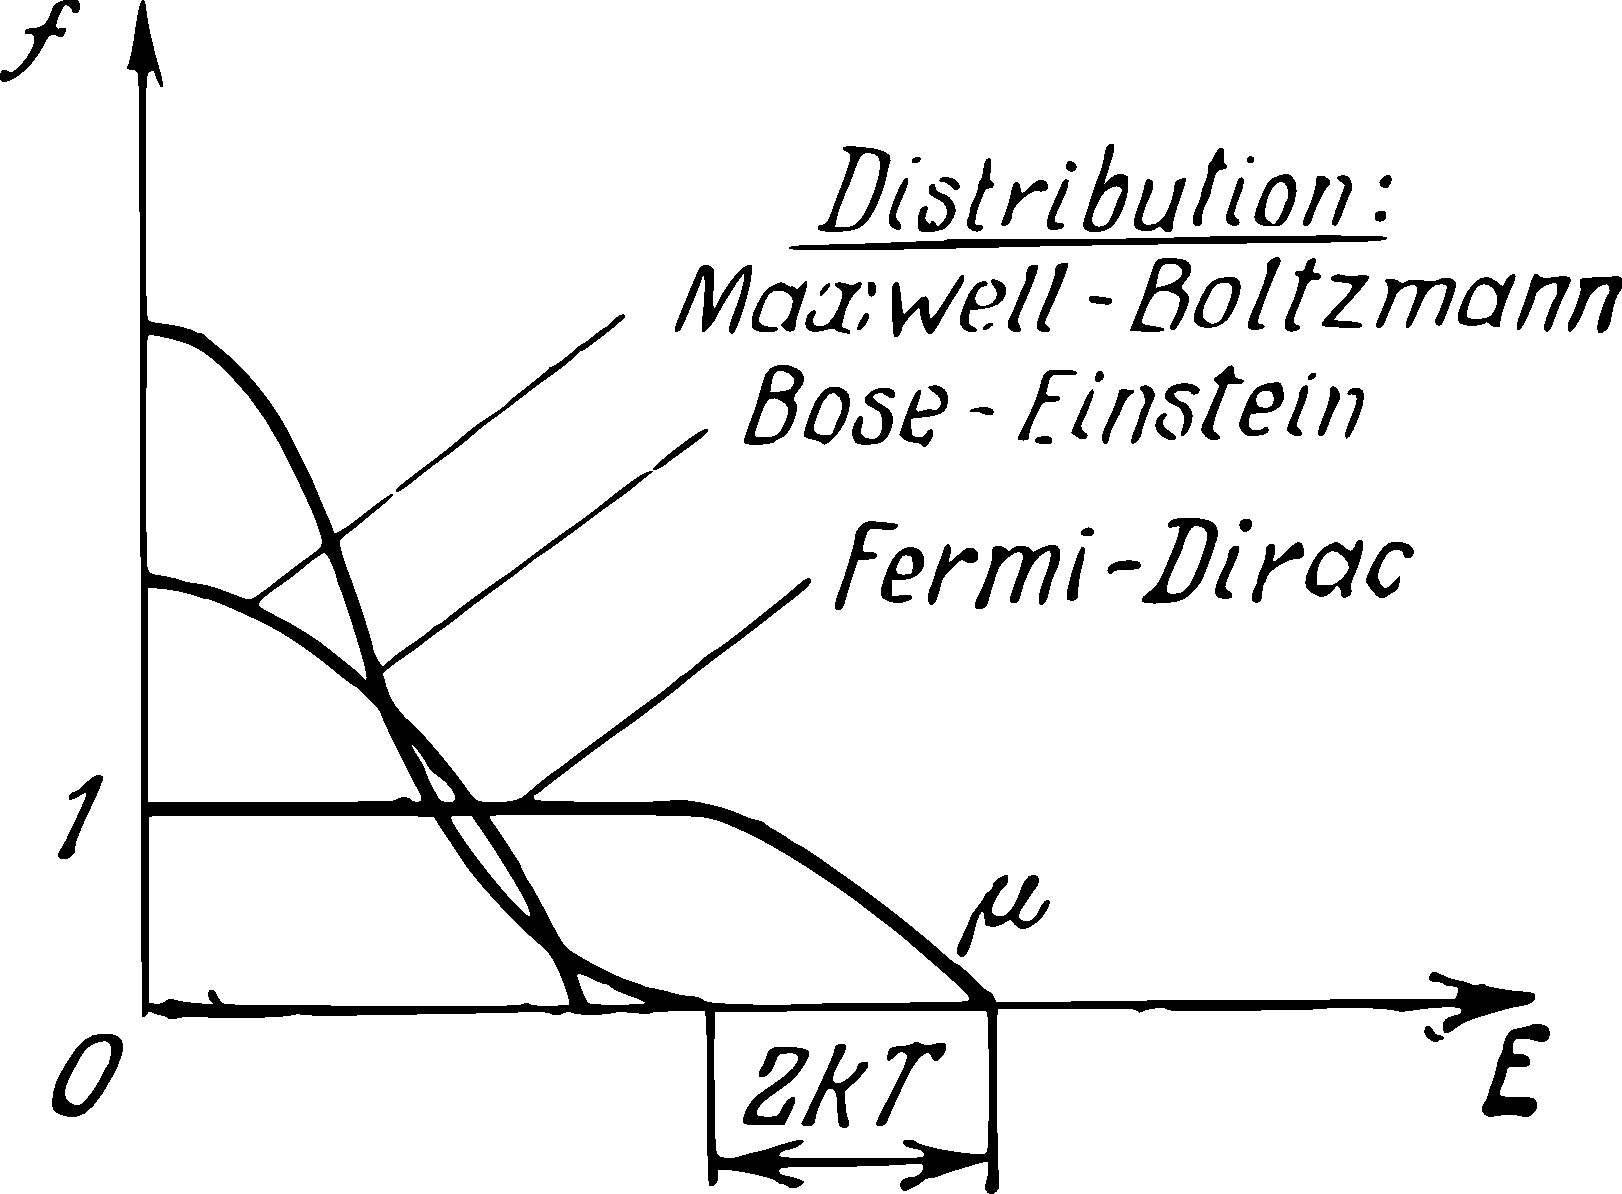
\includegraphics[width=\textwidth]{figs/ch-41/fig-41-01.pdf}
\sidecaption{Comparing the Maxwell-Boltzmann, Bose-Einstein, and Fermi-Dirac distributions.\zhcap{麦克斯韦-玻尔兹曼分布、玻色-爱因斯坦分布与费米-狄拉克分布的比较。}\label{fig-41-01}}
\end{marginfigure}

\textbf{Example.} Blackbody radiation \ssect{36.1.8} is enclosed in a cavity of volume $V$ at $T = \text{const}$, the radiation being in a state of thermodynamic equilibrium with the walls of the cavity. This radiation can be dealt with as a photon gas complying with Bose-Einstein statistics, because the spin of a photon equals $\hbar$ (\tabl{tab-43.1}). The number of quantum states of radiation in volume $V$ \ssect{40.1.4} is
\zhpar{\textbf{例。}体积为 $V$ 的空腔内的黑体辐射（\ssect{36.1.8}），在温度 $T = \text{const}$ 下与空腔壁处于热力学平衡状态。这种辐射可以看作遵从玻色-爱因斯坦统计的光子气体，因为光子的自旋等于 $\hbar$（见\tabl{tab-43.1}）。体积 $V$ 中辐射的量子态数（\ssect{40.1.4}）为：}
\begin{equation*}%
\dd g = 2 \frac{4 \pi p^{2} \dd pV}{h^{3}} = \frac{8\pi E^{2} \dd E}{h^{3}c} V,
\end{equation*}
where $p$ is the momentum of the photon \ssect{37.2.2}, related to its energy by the equation $p = E/c$, where $c$ is the velocity of light in free space. The factor 2 appears because there are two possible directions in which light can be polarized \ssect{31.1.8}. The energy of the photon is $E = h\nu$ \ssect{37.1.4}, where $\nu$ is the frequency. According to section \ssect{41.2.2}, the number of photons with frequencies in the range from $\nu$ to $\nu + \dd \nu$ in the volume $V$ is
\zhpar{式中 $p$ 为光子的动量（\ssect{37.2.2}），它与能量的关系为 $p = E/c$，其中 $c$ 为真空中的光速。因子 2 来源于光可以有两个可能的偏振方向（\ssect{31.1.8}）。光子的能量为 $E = h\nu$（\ssect{37.1.4}），其中 $\nu$ 为频率。根据\ssect{41.2.2}，体积 $V$ 中频率在 $\nu$ 到 $\nu + \dd \nu$ 范围内的光子数为：}
\begin{equation*}%
\dd N = \frac{\dd g}{\exp \left(\dfrac{h \nu}{kT} \right) -1} = \frac{8 \pi \nu^{2} \dd \nu V}{c^{3} [\exp \left(\dfrac{h \nu}{kT} \right) -1]}.
\end{equation*}
Taken into account here is the fact that the chemical potential $\mu$ \ssect{41.2.3} is equal to zero for a photon gas in which the condition for conserving the total number of particles is not complied with.
\zhpar{这里考虑了这样一个事实：对于光子气体，粒子总数不守恒，因此化学势 $\mu$（\ssect{41.2.3}）等于零。}

The volume density of radiant energy in the frequency range
from $\nu$ to $\nu + \dd \nu$ is
\zhpar{在频率范围 $\nu$ 到 $\nu + \dd \nu$ 内，黑体辐射的体积能量密度为：}
\begin{equation*}%
\omega (\nu, \, T) = \frac{h \nu \dd N}{V} = \frac{8 \pi \nu^{2}}{c^{3}} \frac{h \nu \dd \nu}{\exp \left(\dfrac{h \nu}{kT} \right) -1}.
\end{equation*}
This result is Planck's radiation formula for the volume energy density of blackbody radiation \ssect{36.1.5}.
\zhpar{这一结果即为黑体辐射体积能量密度的普朗克辐射公式（\ssect{36.1.5}）。}

\section[Degeneracy of Systems]{Degeneracy of Systems of Particles Described by Quantum Statistics}
\label{sec-41.3} 
\zhtitle{用量子统计描述的粒子系统的简并}

\subsection{}\label{41.3.1} A system of particles (in particular, an ideal gas) is said to be \redem{degenerate} if its properties, described by quantum laws, differ from those of ordinary systems that obey classical laws. Deviation in the behaviour of Bose and Fermi gases from that of classical Maxwellian-Boltzmann gas is called \redem{gas degeneracy}.
This becomes appreciable at extremely low temperatures and high densities \ssect{41.3.3}.
\zhpar{若粒子系统（特别是理想气体）的性质由量子规律描述，且与服从经典规律的普通系统不同，则称该系统是\redem{简并的}。玻色气体和费米气体的行为偏离经典的麦克斯韦-玻尔兹曼气体，这种偏离称为\redem{气体简并}。气体简并在极低温度和高密度下变得显著（\ssect{41.3.3}）。}

\subsection{}\label{41.3.2} The \redem{degeneracy parameter} $A$ is the quantity
\zhpar{\redem{简并参数} $A$ 定义为：}
\begin{equation*}%
A = \exp \left( \frac{\mu}{hT}\right),
\end{equation*}
where $\mu$ is the chemical potential \ssect{41.2.3}. Under the condition of slight degeneracy $(A \ll 1)$, the ones in the denominators of the quantum distribution functions $f_{B}$ and $f_{F}$ can be neglected, and these functions become the classical Maxwellian-Boltzmann distribution function $f_{M\! - \!B}$ Thus
\zhpar{式中 $\mu$ 为化学势（\ssect{41.2.3}）。在弱简并条件 $(A \ll 1)$ 下，量子分布函数 $f_{B}$ 和 $f_{F}$ 分母中的 $\pm 1$ 项可以略去，这两个函数即变为经典的麦克斯韦-玻尔兹曼分布函数 $f_{M\! - \!B}$。由此有：}
\begin{equation*}%
f_{M\! - \!B} = A \exp \left(- \frac{E_{i}}{kT}\right).
\end{equation*}
The degeneracy parameter is found from the condition of normalization of the distribution function: $\sum_{i} \Delta N_{i} = N$ \ssect{41.2.2}, which indicates the conservation of the total number of particles in the system. The condition for slight degeneracy is of the form 
\zhpar{简并参数由分布函数的归一化条件 $\sum_{i} \Delta N_{i} = N$（\ssect{41.2.2}）求得，该条件表示系统中粒子总数守恒。弱简并的条件为：}
\begin{equation*}%
A = \frac{n_{0}h^{3}}{(2 \pi m kT)^{3/2}} \ll 1.
\end{equation*}
where $n_{0}$ is the concentration of particles, $m$ is the mass of the particles, $k$ is Boltzmann's constant, $h$ is Planck's constant, and $T$ is the absolute temperature.
\zhpar{式中 $n_{0}$ 为粒子浓度，$m$ 为粒子质量，$k$ 为玻尔兹曼常量，$h$ 为普朗克常量，$T$ 为热力学温度。}

\subsection{}\label{41.3.3} The \redem{degeneracy temperature} $T_{d}$ is the temperature at which degeneracy becomes appreciable \ssect{41.3.1}. It is determined
from the condition
\zhpar{\redem{简并温度} $T_{d}$ 是简并效应变得显著的温度（\ssect{41.3.1}）。它由下列条件确定：}
\begin{align*}%
A & = \frac{n_{0}h^{3}}{(2 \pi m kT_{d})^{3/2}} = 1, \text{ from which}\\
T_{d} & = \frac{h^{2}n_{0}^{2/3}}{2 \pi mk}.
\end{align*}
The temperature criterion of degeneracy is as follows: when
$T \ll T_{d}$ the system of particles is degenerate; when $T \gg T_{d}$ the system of particles is not degenerate, and its behaviour is described by classical laws.
\zhpar{简并的温度判据如下：当 $T \ll T_{d}$ 时，粒子系统是简并的；当 $T \gg T_{d}$ 时，粒子系统不简并，其行为遵从经典规律。}

For example, the degeneracy parameter $A \approx \num{3d-5} \ll 1$ for hydrogen under standard conditions ($T = \SI{300}{\kelvin}$ and $n_{0} \approx \SI{3d25}{\per\meter\cubed}$). The degeneracy temperature for hydrogen is $T_{d} \approx \SI{1}{\kelvin}$. For all other gases, heavier than hydrogen, $A$ is even smaller. Under standard conditions gases are not degenerate. Degeneracy, associated with the quantum properties of gases, is manifested to a considerably less degree than the deviations of gases from an ideal gas, which is due to intermolecular interaction. Photon gas is always degenerate $(T_{d} = \infty)$ because the rest mass of a photon equals zero ($m_{0} = 0$, \tabl{tab-43.1}). Photon gas is described by Bose-Einstein quantum statistics \ssect{41.2.6}.
\zhpar{例如，在标准状况（$T = \SI{300}{\kelvin}$，$n_{0} \approx \SI{3d25}{\per\meter\cubed}$）下，氢气的简并参数 $A \approx \num{3d-5} \ll 1$。氢气的简并温度约为 $T_{d} \approx \SI{1}{\kelvin}$。对于其他比氢重的气体，$A$ 更小。在标准状况下，气体都不是简并的。与气体量子性质相关的简并效应，远不如由分子间相互作用引起的气体偏离理想气体的程度显著。光子气体总是简并的（$T_{d} = \infty$），因为光子的静止质量为零（$m_{0} = 0$，见\tabl{tab-43.1}）。光子气体遵从玻色-爱因斯坦量子统计（\ssect{41.2.6}）。}

\subsection{}\label{41.3.4} Electrons in metals are an example of a degenerate gas. Under ordinary conditions $n_{0} \approx \num{d28}$ to \SI{d29}{\per\meter\cubed}. Since the mass of the electron is small $(m \approx \SI{d-30}{\kilo\gram})$, $T_{d} \approx (16 \text{ to } 20) \SI{d3}{\kelvin}$. Electron gas does not comply with the classical Maxwell-Boltzmann statistics.
\zhpar{金属中的电子是简并气体的一个例子。在通常条件下，$n_{0} \approx \num{d28}$ 至 \SI{d29}{\per\meter\cubed}。由于电子质量很小（$m \approx \SI{d-30}{\kilo\gram}$），其 $T_{d} \approx (16 \text{ to } 20) \SI{d3}{\kelvin}$。电子气体不服从经典的麦克斯韦-玻尔兹曼统计。}

\subsection{}\label{41.3.5} The energy of degenerate electron gas \ssect{41.4.5}, and other gases described by quantum statistics, is not a linear function of the temperature. Therefore, the simple physical interpretation of the absolute temperature \ssect{8.3.4} is not suitable in the region of degenerate gases \ssect{41.3.3}.
\zhpar{简并电子气（\ssect{41.4.5}）以及其他遵从量子统计的气体，其能量并非温度的线性函数。因此，在简并气体范围内，对热力学温度（\ssect{8.3.4}）的简单物理解释并不适用（\ssect{41.3.3}）。}

\section{Degenerate Electron Fermi Gas in Metals}
\label{sec-41.4} 
\zhtitle{金属中简并的费米电子气}

\subsection{}\label{41.4.1} The energy distribution of conduction electrons in metals is described by the Fermi-Dirac distribution function \ssect{41.2.5}:
\zhpar{金属中导电电子的能量分布由费米-狄拉克分布函数（\ssect{41.2.5}）描述：}
\begin{equation*}%
f_{F} = \frac{1}{\exp \left(\dfrac{E - \mu}{kT} \right) +1}.
\end{equation*}
The number of quantum states of electrons per unit volume of
metal, within the energy range from $E$ to $E + \dd E$ \ssect{41.1.4} is
\zhpar{单位体积金属中，能量在 $E$ 到 $E + \dd E$ 范围内的电子量子态数（\ssect{41.1.4}）为：}
\begin{equation*}%
\dd g(E) = \frac{\dd \Gamma}{h^{3}} =\frac{4 \pi^{2 } \dd p}{h^{3}}= \frac{2 \pi (2m)^{3/2} \sqrt{E} \dd E}{h^{3}}.
\end{equation*}
Use is made here of the relation between the momentum $p$ of
the electron and its energy:
\zhpar{这里用到了电子动量 $p$ 与其能量之间的关系：}
\begin{equation*}%
p^{2} = 2mE, \quad \dd p = \sqrt{\frac{m}{2E}} \dd E.
\end{equation*}
The number of electrons $\dd n_{0} (E)$ in unit volume of the metal, having energies within the range from $E$ to $E + \dd E$ equals, according to \ssect{41.2.2}:
\zhpar{单位体积金属中能量在 $E$ 到 $E + \dd E$ 范围内的电子数 $\dd n_{0} (E)$，根据\ssect{41.2.2}，等于：}
\begin{equation*}%
\dd n_{0} (E) = 2 f_{F} \dd g(E)  = \frac{4 \pi (2m)^{3/2}}{h^{3}} \, \frac{\sqrt{E} \dd E}{\exp \left(\dfrac{E - \mu}{kT} \right) + 1}.
\end{equation*}
Factor 2 takes into account the fact that the electrons comply with the Pauli exclusion principle \ssect{39.3.1}. This equation expresses the energy distribution law for conduction electrons in a metal.
\zhpar{因子 2 考虑了电子遵守泡利不相容原理（\ssect{39.3.1}）这一事实。该式即为金属中导电电子的能量分布规律。}

\subsection{}\label{41.4.2} The unusual properties of electron gas have an effect on its behaviour at the absolute zero temperature $(T = \SI{0}{\kelvin})$. If $\mu_{0}$ is the chemical potential of the gas at $T = \SI{0}{\kelvin}$ \ssect{41.2.3}, then
\zhpar{电子气体的特殊性质影响其在绝对零度 $(T = \SI{0}{\kelvin})$ 时的行为。若 $\mu_{0}$ 为气体在 $T = \SI{0}{\kelvin}$ 时的化学势（\ssect{41.2.3}），则有：}
\begin{equation*}%
f_{F} = \frac{1}{\exp \left(\dfrac{E - \mu_{0}}{kT} \right) +1}.
\end{equation*}
at $E < \mu_{0}$ the difference $E - \mu_{0} < 0$ and
\zhpar{当 $E < \mu_{0}$ 时，差值 $E - \mu_{0} < 0$，且}
\begin{equation*}%
f_{F} = \frac{1}{\dfrac{1}{\exp \left(\dfrac{ \mu_{0} - E}{kT} \right) +1}};
\end{equation*}
at $E - \mu_{0} < 0$ and $T \to 0$, $\exp [(\mu_{0} - E)/kT] \to \infty$ and $f_{F} \to 1$; at $E > \mu_{0}$, the difference $ E - \mu_{0} > 0$ and at $T \to 0$, $\exp [(E - \mu_{0})/kT] \to  \infty$ and $f_{F} \to 0$.
\zhpar{当 $E - \mu_{0} < 0$ 且 $T \to 0$ 时，$\exp [(\mu_{0} - E)/kT] \to \infty$，故 $f_{F} \to 1$；当 $E > \mu_{0}$ 时，差值 $E - \mu_{0} > 0$，且当 $T \to 0$ 时，$\exp [(E - \mu_{0})/kT] \to \infty$，故 $f_{F} \to 0$。}




The curve of the Fermi distribution function fp at $T = \SI{0}{\kelvin}$ is given in \figr{fig-41-02}. In the energy range from 0 to $\mu_{0}$, function $f_{F}$ is equal to unity. In passing through the value $E = \mu_{0}$, the function drops abruptly to zero. At $T = \SI{0}{\kelvin}$, the electrons of the metal occupy all allowed energy levels with a population equal to unity \ssect{41.2.2} up to the level with the energy $E = \mu_{0}$.
\zhpar{费米分布函数 $f_{F}$ 在 $T = \SI{0}{\kelvin}$ 时的曲线如\figr{fig-41-02}所示。在 $0$ 到 $\mu_{0}$ 的能量范围内，函数 $f_{F}$ 等于 1。当能量经过 $E = \mu_{0}$ 时，函数突然降为零。在 $T = \SI{0}{\kelvin}$ 时，金属中的电子以占据数 1 占据直到能量为 $E = \mu_{0}$ 的所有允许能级（\ssect{41.2.2}）。}


All levels with energy exceeding $\mu_{0}$ are empty; their population equals zero. Thus, $\mu_{0}$ is the maximum energy that conduction electrons can have at absolute zero temperature. This quantity is called the \redem{Fermi energy}: $\mu_{0} = E_{F}$. If the consecutive numbers of the energy levels are plotted along the axis of abscissas in \figr{fig-41-02}, and the corresponding numbers of conduction electrons per unit volume are the ordinates, the maximum ordinate corresponds to the energy level number $n_{0}/2$, where $n_{0}$ is the electron concentration. The highest level occupied by electrons is called the \redem{Fermi level}. It corresponds to the Fermi energy $E_{F}$, which an electron has at this level.
\zhpar{所有能量超过 $\mu_{0}$ 的能级都是空的，其占据数为零。因此，$\mu_{0}$ 是导电电子在绝对零度时所能具有的最大能量。这一量称为\redem{费米能量}：$\mu_{0} = E_{F}$。若在\figr{fig-41-02}中以能级序号为横坐标、以相应单位体积中的导电电子数为纵坐标，则纵坐标的最大值对应于能级序号 $n_{0}/2$，其中 $n_{0}$ 为电子浓度。电子所占据的最高能级称为\redem{费米能级}，它对应于电子在该能级上所具有的费米能量 $E_{F}$。}

\begin{marginfigure}[-4cm] 
\centering
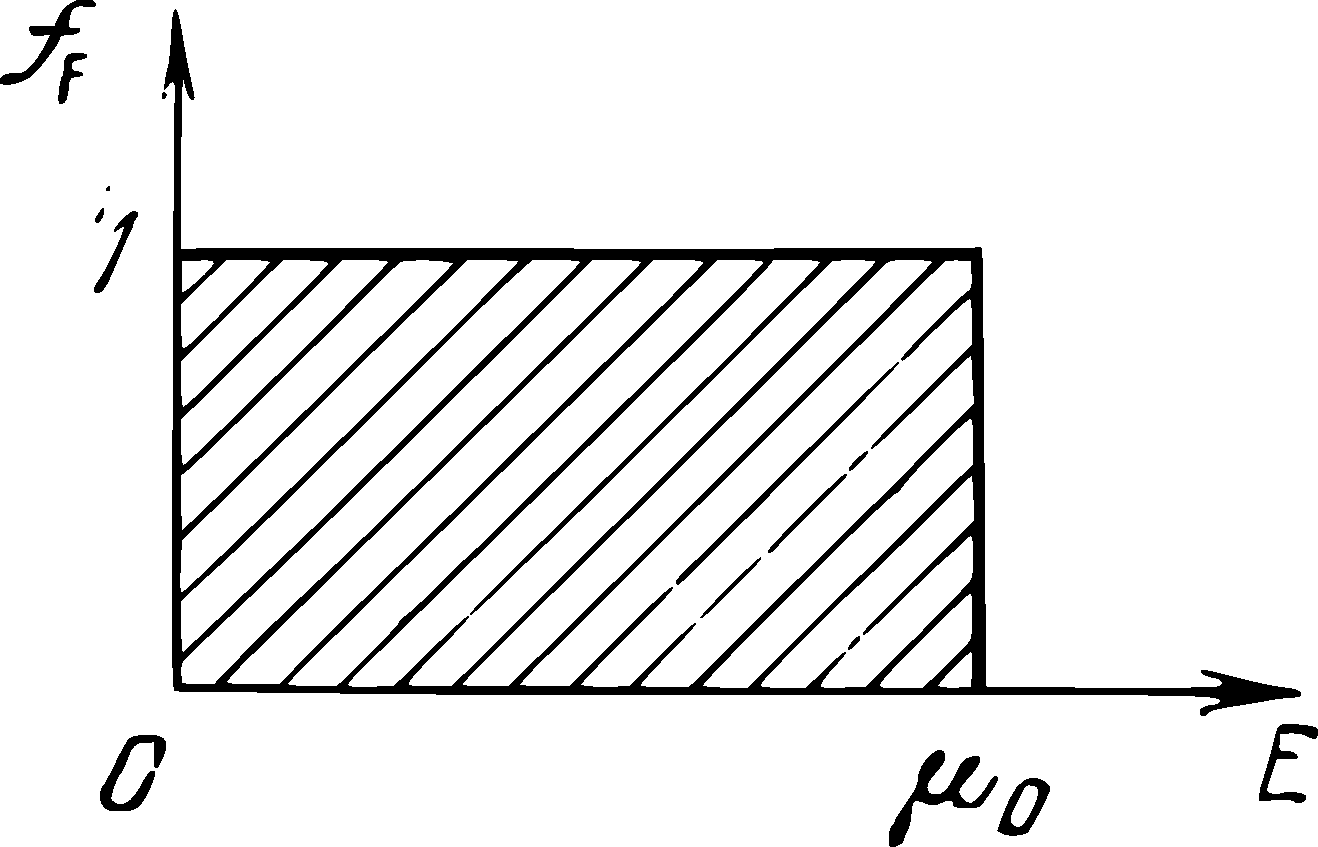
\includegraphics[width=\textwidth]{figs/ch-41/fig-41-02.pdf}
\sidecaption{The Fermi distribution function.\zhcap{费米分布函数。}\label{fig-41-02}}
\end{marginfigure}




\subsection{}\label{41.4.3} The energy distribution law for conduction electrons at $T = \SI{0}{\kelvin}$ is of the form
\zhpar{导电电子在 $T = \SI{0}{\kelvin}$ 时的能量分布规律为：}
\begin{equation*}%
\dd n_{0}(E) = \frac{4\pi (2m)^{3} \sqrt{E} \dd E}{h^{3}}
\end{equation*}
It is represented graphically by the curve in \figr{fig-41-03}.
The total number of conduction electrons in unit volume of
a metal is
\zhpar{其图像如\figr{fig-41-03}中的曲线所示。单位体积金属中导电电子的总数为：}
\begin{align*}%
 n_{0} & = \int_{0}^{E_{F}} \dd n_{0} (E) = \frac{4\pi (2m)^{3} }{h^{3}} \int_{0}^{E_{F}} \sqrt{E} \dd E \\
 & = \frac{4\pi (2m)^{3} }{h^{3}} \frac{2}{3} E_{F}^{3/2}.
\end{align*}
\begin{marginfigure}[2cm] 
\centering
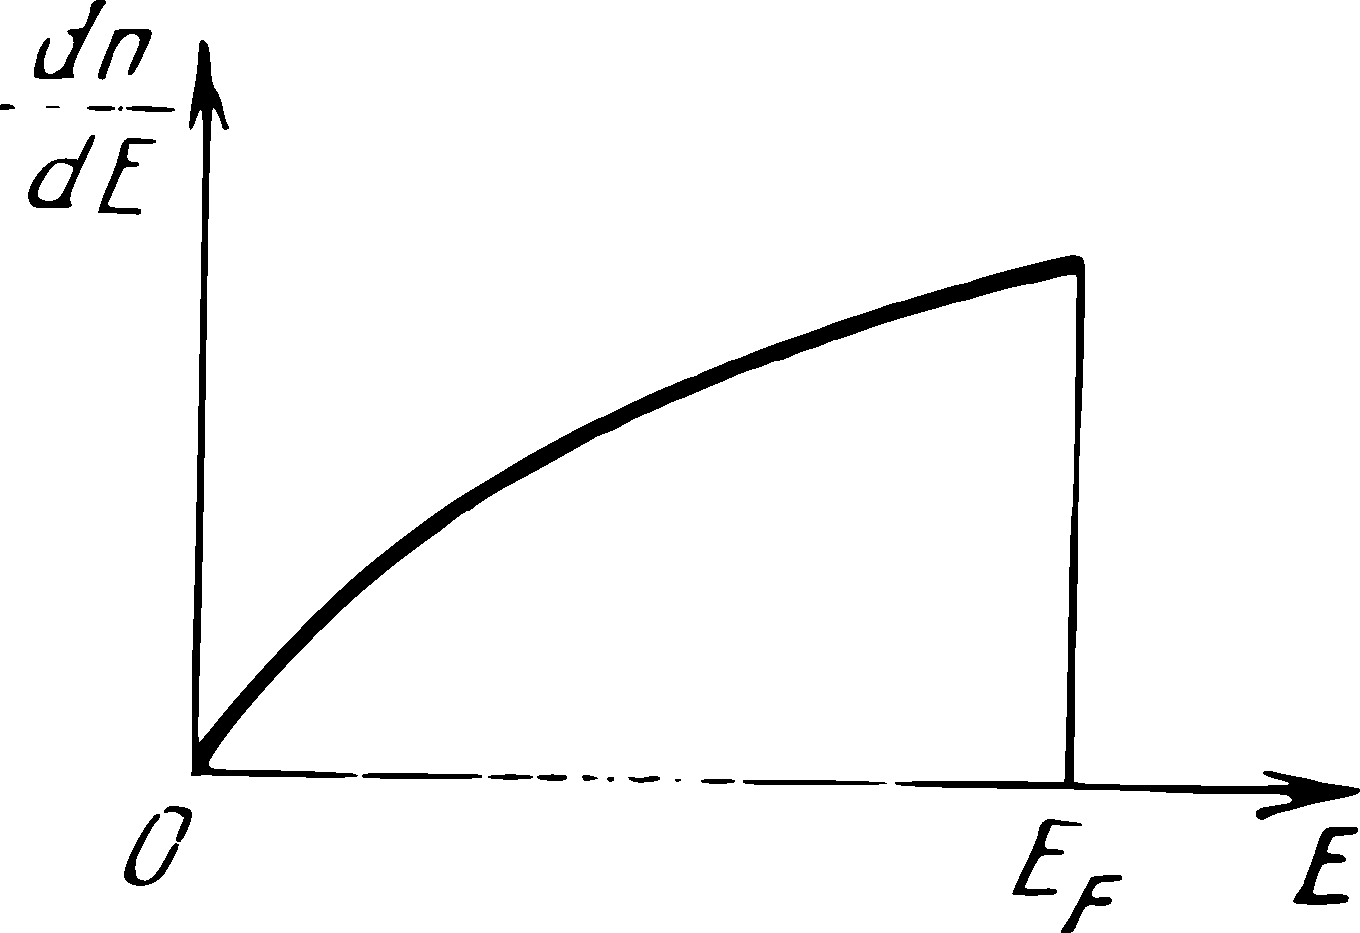
\includegraphics[width=\textwidth]{figs/ch-41/fig-41-03.pdf}
\sidecaption{The energy distribution law for conduction electrons at $T = \SI{0}{\kelvin}$.\zhcap{导电电子在 $T = \SI{0}{\kelvin}$ 时的能量分布规律。}\label{fig-41-03}}
\end{marginfigure}
Hence
\zhpar{由此得：}
\begin{equation*}%
E_{F} = \frac{h^{2}}{2m} \left( \frac{3 n_{0}}{8\pi}\right)^{2/3}.
\end{equation*}
The average energy $\expval{E}$ of the electron at $T = \SI{0}{\kelvin}$ is
\zhpar{电子在 $T = \SI{0}{\kelvin}$ 时的平均能量 $\expval{E}$ 为：}
\begin{equation*}%
\expval{E} = \frac{3}{5} E_{F} = \frac{3}{5} \frac{h^{2}}{2m} \left( \frac{3 n_{0}}{8\pi}\right)^{2/3}.
\end{equation*}
At $n_{0} = \SI{6d-28}{\per\meter\cubed}$ we obtain, after substituting the values of $h$ and $m$:
\zhpar{当 $n_{0} = \SI{6d-28}{\per\meter\cubed}$ 时，代入 $h$ 和 $m$ 的数值后得到：}
\begin{equation*}%
\expval{E} = \SI{9d-19}{\joule} = \SI{5.4}{\electronvolt}.
\end{equation*}
If we compare this energy with the average energy of a molecule of nondegenerate monatomic gas $\expval{E} = 3kT/2$ \ssect{10.2.5}, we find the energy $E_{F}$ that the molecule could have at the temperature $T  \approx \SI{d4}{\kelvin}$. In other words, under ordinary conditions, $kT/E_{F} \ll 1$.
\zhpar{若将此能量与非简并单原子气体分子的平均能量 $\expval{E} = 3kT/2$（\ssect{10.2.5}）相比较，便可求出该分子在温度 $T \approx \SI{d4}{\kelvin}$ 时所具有的能量 $E_{F}$。换言之，在通常条件下，$kT/E_{F} \ll 1$。}

\subsection{}\label{41.4.4} At a temperature different from zero the Fermi-Dirac distribution function $f_{F}$ is of the form shown in \figr{fig-41-04} by the full-line curve. The same figure shows the function  $f_{F}$ at $T = \SI{0}{\kelvin}$ in dash lines. The curves differ in the kind of drop the function undergoes near the value $E = \mu$. 
\zhpar{在非零温度下，费米-狄拉克分布函数 $f_{F}$ 的形状如\figr{fig-41-04}中的实线曲线所示，同一图中的虚线表示 $T = \SI{0}{\kelvin}$ 时的函数 $f_{F}$。两条曲线的区别在于函数在 $E = \mu$ 附近的下降方式不同。}

An abrupt drop along a vertical line at $E = \mu_{0} = E_{F}$ for the case when $T = \SI{0}{\kelvin}$ (\figr{fig-41-02}) changes to the smooth curve $ABC$ at $T \neq \SI{0}{\kelvin}$. Of importance is the fact that the states of the electrons, at the energy levels that satisfy the condition $E \ll \mu$, do not change when heated from \SI{0}{\kelvin} to $T$. Distortion of the function $f_{F}$ occurs only at its ``tail-end'', in an energy range of the width $2 k T$, near the value $E = \mu$, at which $f_{F} = 1/2$.
\zhpar{在 $T = \SI{0}{\kelvin}$ 时（见\figr{fig-41-02}），在 $E = \mu_{0} = E_{F}$ 处的竖直陡降，在 $T \neq \SI{0}{\kelvin}$ 时变为光滑曲线 $ABC$。值得注意的是，能量满足 $E \ll \mu$ 条件的能级上的电子状态，在由 $\SI{0}{\kelvin}$ 加热到 $T$ 时并不改变。函数 $f_{F}$ 的畸变只发生在其“尾部”，即在 $E = \mu$ 附近宽度为 $2 k T$ 的能量范围内，而在 $E = \mu$ 处 $f_{F} = 1/2$。}
\begin{marginfigure}[-3cm] 
\centering
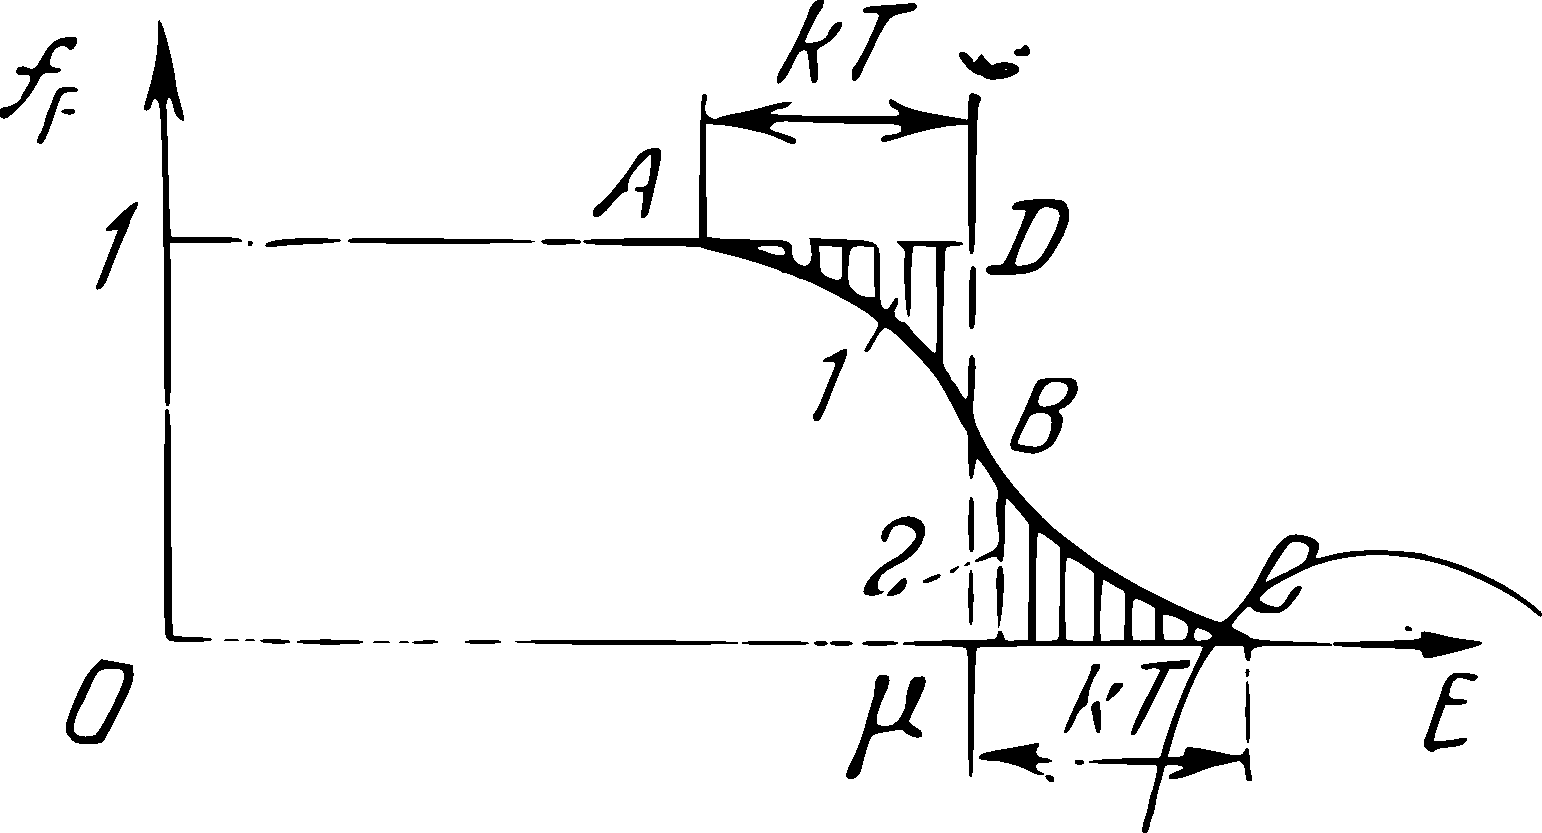
\includegraphics[width=\textwidth]{figs/ch-41/fig-41-04.pdf}
\sidecaption{Fermi-Dirac distribution at different temperature than $T = \SI{0}{\kelvin}$.\zhcap{不同于 $T = \SI{0}{\kelvin}$ 的温度下的费米-狄拉克分布。}\label{fig-41-04}}
\end{marginfigure}

\subsection{}\label{41.4.5} The chemical potential  $\mu$\ssect{41.2.3} of an electron gas at the temperature $T$ is
\zhpar{温度为 $T$ 时，电子气体的化学势 $\mu$（\ssect{41.2.3}）为：}
\begin{equation*}%
\mu =  E_{F} \left[ 1 - \frac{\pi^{2}}{12} \left( \frac{kT}{E_{F}}\right)^{2} \right].
\end{equation*}
The internal energy $U$ \ssect{9.1.2} of a mole of electron gas is
\zhpar{一摩尔电子气体的内能 $U$（\ssect{9.1.2}）为：}
\begin{equation*}%
U =  \frac{3}{5} N_{A}E_{F}  \left[ 1 + \frac{15}{12}  \frac{\pi^{2} (kT)^{2}}{E_{F}^{2}} \right].
\end{equation*}
Here $N$ is Avogadro's number (Appendix~II), and $k$ is Boltzmann's constant \ssect{8.4.5}. Quantities $\mu$ and $U$ remain practically constant when the temperature is raised.
\zhpar{式中 $N$ 为阿伏伽德罗常量（附录II），$k$ 为玻尔兹曼常量（\ssect{8.4.5}）。当温度升高时，量 $\mu$ 和 $U$ 实际上保持不变。}

The molar heat capacity $C_{V \mu}$ \ssect{9.5.2} of an electron gas is 
\zhpar{电子气体的摩尔热容 $C_{V \mu}$（\ssect{9.5.2}）为：}
\begin{equation*}%
C_{V\mu} =  \pdv{U}{T} = \frac{\pi^{2}}{2} N_{A}k \frac{kT}{E_{F}}.
\end{equation*}
A comparison with the heat capacity of a nondegenerate monatomic gas \ssect{10.7.1} $C^{\text{class}}_{V \mu} = 3 N_{A}k/2$, indicates that
\zhpar{将其与非简并单原子气体的热容（\ssect{10.7.1}）$C^{\text{class}}_{V \mu} = 3 N_{A}k/2$ 相比较，可知：}
\begin{equation*}%
\frac{C_{V\mu}}{C^{\text{class}}_{V \mu}} =   \frac{\pi^{3}}{3} \frac{kT}{E_{F}}.
\end{equation*}
At room temperature $kT/E_{F}  \approx 0.01$ \ssect{41.4.3}, and therefore $C_{V\mu}/C^{\text{class}}_{V \mu} \approx 0.03$. The heat capacity of degenerate electron gas is negligibly small. This is so because only a slight number of electrons, within the ``drop region'' of the Fermi-Dirac distribution function $f_{F}$ (hatched regions $\mathit{1}$ and $\mathit{2}$ in \figr{fig-41-04}), participate in the process of changing the internal energy of the electron gas when it is heated. This removes one of the chief shortcomings of the classical electron theory of the electrical conduction of metals \ssect{20.3.7}.
\zhpar{在室温下 $kT/E_{F} \approx 0.01$（\ssect{41.4.3}），因此 $C_{V\mu}/C^{\text{class}}_{V \mu} \approx 0.03$。简并电子气体的热容可以忽略不计。这是因为，在加热时，只有位于费米-狄拉克分布函数“下降区域”内（见\figr{fig-41-04}中的阴影区域 $\mathit{1}$ 和 $\mathit{2}$）的少量电子参与改变电子气体的内能。这样就消除了金属导电经典电子理论的一个主要缺陷（\ssect{20.3.7}）。}

\section{Quantum Theory of Electrical Conduction in Metals}
\label{sec-41.5} 
\zhtitle{金属导电的量子理论}


\subsection{}\label{41.5.1} The theory of the electrical conduction of metals, based on quantum mechanics \ssect{38.1.1} and Fermi-Dirac quantum statistics
\ssect{41.2.5} is called the \redem{quantum theory of electrical conduction in metals}. Using the Fermi-Dirac distribution function \ssect{41.2.5} in this theory, Ohm's law for current density \ssect{20.3.4} was derived. Thus
\zhpar{以量子力学（\ssect{38.1.1}）和费米-狄拉克量子统计（\ssect{41.2.5}）为基础的金属导电理论，称为\redem{金属导电的量子理论}。该理论利用费米-狄拉克分布函数（\ssect{41.2.5}）推导出了电流密度形式的欧姆定律（\ssect{20.3.4}）。即：}
\begin{equation*}%
\vb{j} = \varkappa \vb{E}.
\end{equation*}
\subsection{}\label{41.5.2} In the quantum theory of electrical conduction, the electrical conductivity $\varkappa $ is calculated by the formula
\zhpar{在金属导电的量子理论中，电导率 $\varkappa $ 由下式计算：}
\begin{equation*}%
\varkappa  = \frac{n_{0}e^{2} \expval{\lambda_{F}}}{m u_{F}}.
\end{equation*}
where $n_{0}$ is the number of conduction electrons per unit volume of the metal, $\expval{\lambda_{F}}$ is the mean free path of the electron \ssect{20.3.1} having Fermi energy \ssect{41.4.2}, and $u_{F}$ is the velocity of thermal motion of such an electron. Notwithstanding the external resemblance
between this formula and the formula for $\varkappa$ in the
classical electron theory \ssect{20.3.4}, it has an entirely different physical content and, in contrast to the classical formula, it completely agrees with the experimental data.
\zhpar{式中 $n_{0}$ 为单位体积金属中的导电电子数，$\expval{\lambda_{F}}$ 为具有费米能量（\ssect{41.4.2}）的电子的平均自由程（\ssect{20.3.1}），$u_{F}$ 为该电子的热运动速度。尽管该式在形式上与经典电子理论中的 $\varkappa$ 公式（\ssect{20.3.4}）相似，但其物理内涵完全不同，而且与经典公式相反，它与实验数据完全相符。}

\subsection{}\label{41.5.3} Also explained in the quantum theory of electrical conduction of metals is the dependence of electrical conductivity mi temperature ($\varkappa \propto 1/T$), as well as the anomalously large mean free path of the electron in a metal \ssect{20.3.7}. The ordered motions of electrons in a metal --- electric current --- is dealt with
in quantum theory as the process of propagation of electron
de Broglie waves \ssect{38.1.4} scattered by anharmonic thermal vibrations of the lattice points in the metal \ssect{40.2.4}. 
\zhpar{金属导电的量子理论还解释了电导率对温度的依赖关系（$\varkappa \propto 1/T$），以及金属中电子反常大的平均自由程（\ssect{20.3.7}）。金属中电子的定向运动，即电流，在量子理论中被看作电子德布罗意波（\ssect{38.1.4}）的传播过程，而这些波被金属中格点的非简谐热振动所散射（\ssect{40.2.4}）。}

Analogus phenomenon occurs in optics in the propagation of
wave through a turbid medium, containing scattering (suspended particles in a liquid, colloidal solutions,
\ssect{34.3.1} . When the distance between the scattering centres are of an order comparable to the wavelength, scattering of the light occurs and the intensity of the light decreases as it propagates in the medium. At distances between the scattering centres substantially less than the wavelength, the medium is optically homogeneous and no light scattering occurs.
\zhpar{光学中也有类似的现象：光波在含有散射体的浑浊介质（如液体中的悬浮微粒、胶体溶液，\ssect{34.3.1}）中传播。当散射中心之间的距离与波长同量级时，光发生散射，光在介质中传播时强度减弱。当散射中心之间的距离远小于波长时，介质在光学上是均匀的，不发生光的散射。}

\subsection{}\label{41.5.4} An ideal crystal lattice, free of all violations of periodicity and with stationary particles at the lattice points, behaves like an optically hgmogeneous medium; it does not scatter electron waves and conduction electrons pass through such a lattice without resistance. The scattering of electron waves occurs only when the periodicity of the lattice is violated. These are inhomogeneities that act as scattering centres. Such centres are, for example, density fluctuations in the lattice \ssect{11.6.3}, resulting from anharmonic thermal vibrations of the positive ions of the metal. With the exception of superconductors \ssect{41.6.1} , this scattering is what leads to the existence of electrical resistance in pure metals.
\zhpar{理想晶格没有任何周期性的破坏，其格点上的粒子静止不动，它表现得像光学上均匀的介质：不散射电子波，导电电子通过这种晶格时没有电阻。只有晶格的周期性遭到破坏时，才会发生电子波的散射。这些不均匀性充当散射中心，例如晶格中由金属正离子的非简谐热振动引起的密度涨落（\ssect{11.6.3}）。除超导体（\ssect{41.6.1}）外，正是这种散射导致了纯金属中电阻的存在。}

\subsection{}\label{41.5.5} The scattering of the electron waves by the thermal vibrations of the lattice points increases with the temperature, whereas the mean free path of the electrons is reduced. The quantity $(\expval{\lambda_{F}})$ is calculated by the formula
\zhpar{电子波被格点热振动的散射随温度升高而增强，因此电子的平均自由程减小。量 $(\expval{\lambda_{F}})$ 由下式计算：}
\begin{equation*}%
\expval{\lambda_{F}} = \frac{E\, d}{\pi n_{0} kT}
\end{equation*}
where $E$ is Young's modulus \ssect{40.3.6}, $d$ is the crystal lattice constant, $n_{0}$ is the number of atoms in unit volume, $k$ is Boltzmann's constant \ssect{8.4.5}, and T is the absolute temperature. Here the electrical conductivity is found to be inversely proportional to the absolute temperature and independent of $n_{0}$ for monovalent metals\sidenote{The concentration of conduction electrons and ions in the lattice coincide in such metals.}. Thus
\zhpar{式中 $E$ 为杨氏模量（\ssect{40.3.6}），$d$ 为晶格常量，$n_{0}$ 为单位体积中的原子数，$k$ 为玻尔兹曼常量（\ssect{8.4.5}），$T$ 为热力学温度。在这种情形下，对于一价金属，电导率与热力学温度成反比，且与 $n_{0}$ 无关。由此有：}
\zhpar{注：在这类金属中，导电电子的浓度与晶格中离子的浓度相同。}
\begin{equation*}%
\varkappa =  \frac{e^{2} E\, d}{m u_{F} \pi kT}
\end{equation*}
This formula agrees with experimental data in the region of
room temperatures. The conductivity, for instance, obtained
for silver ($E = \SI{d7}{\newton\per\meter\squared}$, $d = \SI{3d-10}{\meter}$, $E = \SI{d7}{\newton\per\meter\squared}$, $m = \SI{9d-31}{\kilo\gram}$
, $kT = \SI{4.2d-32}{\joule}$, and $u_{F} = \SI{1.4}{\meter\per\second}$) is
 $\varkappa_{\text{theor}} \approx \SI{5d7}{\per\ohm\per\meter}$, whereas  $\varkappa_{\text{exper}} \approx \SI{6.3d7}{\per\ohm\per\meter}$.
\zhpar{该式与室温范围内的实验数据相符。例如对银（$E = \SI{d7}{\newton\per\meter\squared}$，$d = \SI{3d-10}{\meter}$，$E = \SI{d7}{\newton\per\meter\squared}$，$m = \SI{9d-31}{\kilo\gram}$，$kT = \SI{4.2d-32}{\joule}$，$u_{F} = \SI{1.4}{\meter\per\second}$），由此得到的理论电导率为 $\varkappa_{\text{theor}} \approx \SI{5d7}{\per\ohm\per\meter}$，而实验值为 $\varkappa_{\text{exper}} \approx \SI{6.3d7}{\per\ohm\per\meter}$。}

At very low temperatures the formulas given above are not valid. The mean free path under these conditions is inversely proportional to $T^{5}$, which agrees with experimental data.
\zhpar{在极低温度下，上述公式不再成立。此时平均自由程与 $T^{5}$ 成反比，这与实验数据相符。}

\subsection{}\label{41.5.6} Besides density fluctuations, the cause of electron wave scattering and the electrical resistance of metals is violation in the periodicity of the crystal lattice due to the inclusions of impurity atoms in the lattice. The resistivity $\rho$ of a metal ($\rho = 1/\varkappa$) consists of two parts: 
\zhpar{除密度涨落外，电子波散射以及金属电阻的另一原因，是晶格中混入杂质原子，破坏了晶格的周期性。金属的电阻率 $\rho$（$\rho = 1/\varkappa$）由两部分组成：}
\begin{equation*}%
\rho =  \rho_{T} + \rho_{\text{imp}},
\end{equation*}
\begin{marginfigure}[-4cm] 
\centering
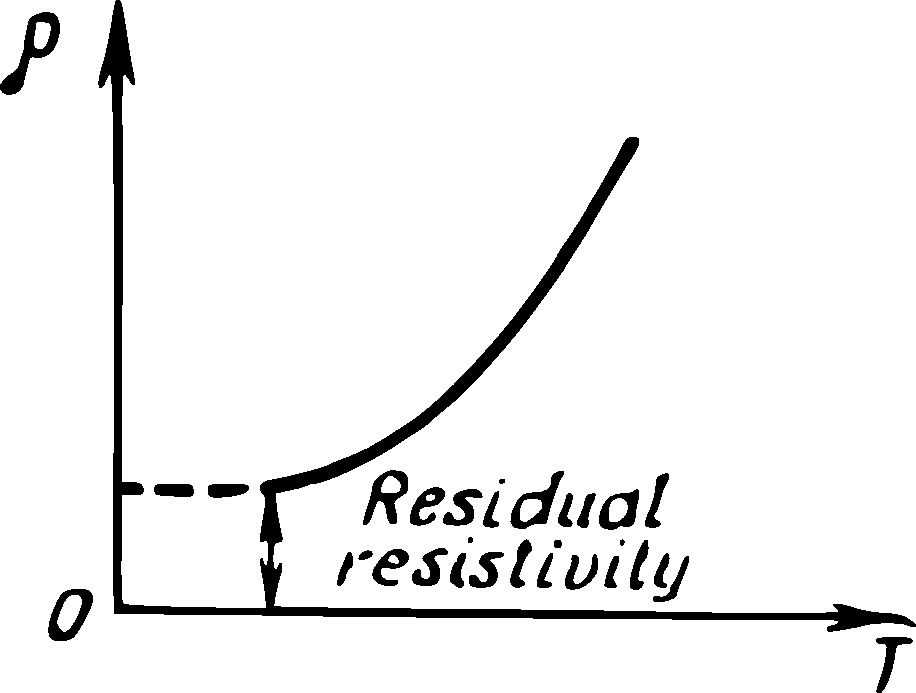
\includegraphics[width=0.8\textwidth]{figs/ch-41/fig-41-05.pdf}
\sidecaption{Resistivity $\rho$ of a metal as a function of the temperature.\zhcap{金属的电阻率 $\rho$ 随温度的变化。}\label{fig-41-05}}
\end{marginfigure}
where $\rho_{T}$ is the resistivity due to the scattering of electron waves by density fluctuations, and $\rho_{\text{imp}}$ is the resistivity due to scattering by impurities. Of importance is the fact that $\rho_{\text{imp}}$ is independent of the temperature. Since as $T \to 0$, $\rho_{T} \to 0$ as well, $\rho_{T} \to \rho_{\text{imp}}$ as the temperature is lowered. The quantity $\rho_{\text{imp}}$ is called the \redem{residual resistivity}. This resistivity remains a property of the metal when it is cooled even down to absolute zero. The dependence of the electrical resistivity on the temperature is shown in \figr{fig-41-05}. The point of intersection of the extension of the curve (dash line) with the axis of ordinates (to $T = \SI{0}{\kelvin}$) is the residual resistivity.
\zhpar{式中 $\rho_{T}$ 为电子波被密度涨落散射所引起的电阻率，$\rho_{\text{imp}}$ 为被杂质散射所引起的电阻率。值得注意的是，$\rho_{\text{imp}}$ 与温度无关。由于当 $T \to 0$ 时 $\rho_{T} \to 0$，因此随着温度降低，$\rho_{T} \to \rho_{\text{imp}}$。量 $\rho_{\text{imp}}$ 称为\redem{剩余电阻率}。即使冷却到绝对零度，这一电阻率仍是金属的固有性质。电阻率随温度的变化关系如\figr{fig-41-05}所示。曲线（虚线）的延长线与纵坐标轴（即 $T = \SI{0}{\kelvin}$ 处）的交点，即为剩余电阻率。}

\section{Superconductivity}
\label{sec-41.6} 
\zhtitle{超导电性}


\subsection{}\label{41.6.1} The \redem{phenomenon of superconductivity} consists in the practically complete disappearance of electrical resiivity in certain metals and alloys at a certain temperature $T_{c}$, called the \redem{transition temperature to a superconductive state}. Substances having this property are called \redem{superconductors}. Today over 500 pure elements and alloys are known that display superconductivity.
\zhpar{\redem{超导现象}是指某些金属和合金在特定温度 $T_{c}$ 下电阻率几乎完全消失。该温度称为\redem{超导态转变温度}。具有这种性质的物质称为\redem{超导体}。目前已知有超过 500 种纯元素和合金表现出超导电性。}

\begin{marginfigure}%[-3cm] 
\centering
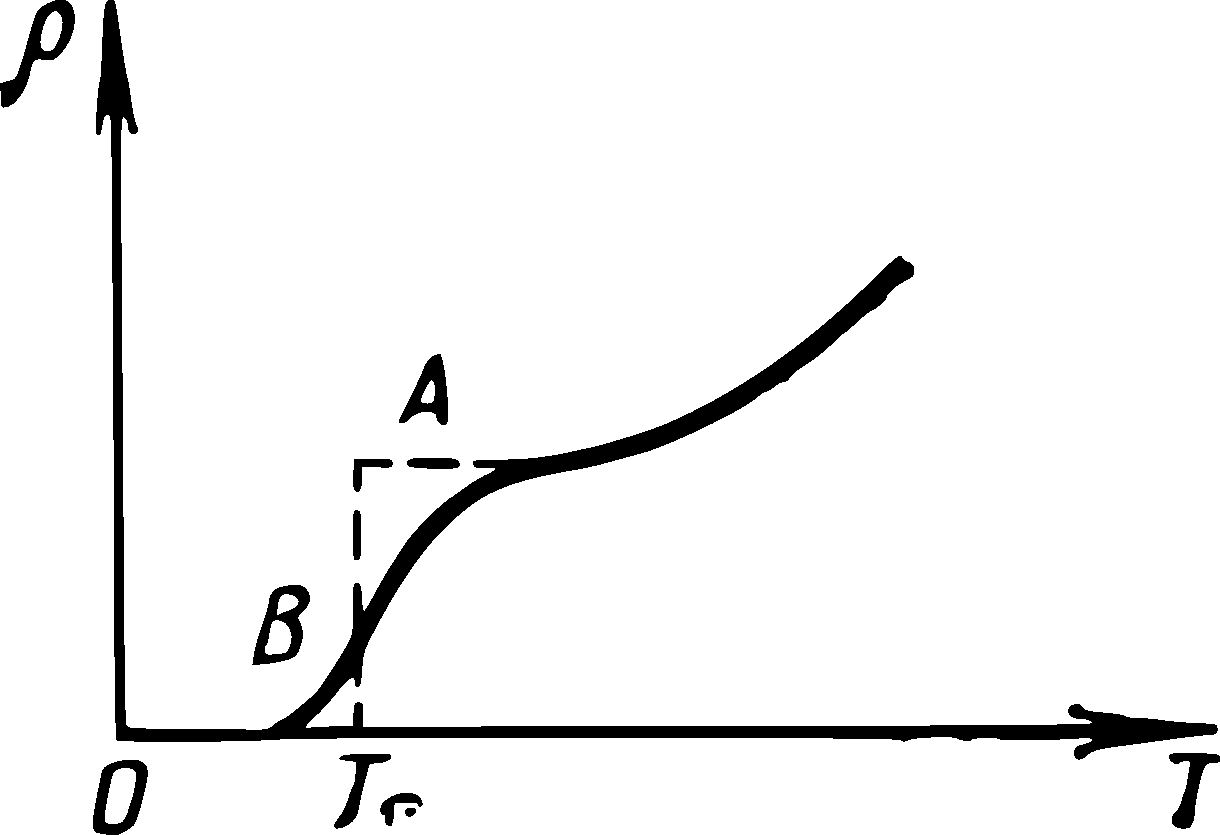
\includegraphics[width=0.9\textwidth]{figs/ch-41/fig-41-06.pdf}
\sidecaption{The temperature range of superconducting state.\zhcap{超导态的温度范围。}\label{fig-41-06}}
\end{marginfigure}

The temperature range $AB$ (\figr{fig-41-06}) of the transition to a superconductive state does not exceed thousandths of a degree for pure specimens. It therefore proves expedient to assign a definite value to $T_{c}$. The width of the range $AB$ depends on nonhomogeneities in the metal, primarily on the presence of impurities and internal stresses in the specimen. The temperatures $T_{c}$ known at the present time range from \SI{0.155}{\kelvin} (\ce{BiPt}) to \SI{23.2}{\kelvin} (\ce{Nb3Ge}).
\zhpar{对于纯净样品，向超导态转变的温度范围 $AB$（见\figr{fig-41-06}）不超过千分之几度。因此，为 $T_{c}$ 赋予一个确定的值是恰当的。范围 $AB$ 的宽度取决于金属中的不均匀性，主要是样品中杂质和内应力的存在。目前已知的 $T_{c}$ 值范围从 \SI{0.155}{\kelvin}（\ce{BiPt}）到 \SI{23.2}{\kelvin}（\ce{Nb3Ge}）。}

The \redem{isotope effect} in superconductors is the fact that the transition temperatures $T_{c}$ of various isotopes \ssect{42.1.3} of the same superconducting metal are inversely proportional to the square roots of their atomic masses.
\zhpar{超导体中的\redem{同位素效应}是指：同一超导金属的不同同位素（\ssect{42.1.3}）的转变温度 $T_{c}$ 与其原子质量的平方根成反比。}

\begin{marginfigure}%[-2cm] 
\centering
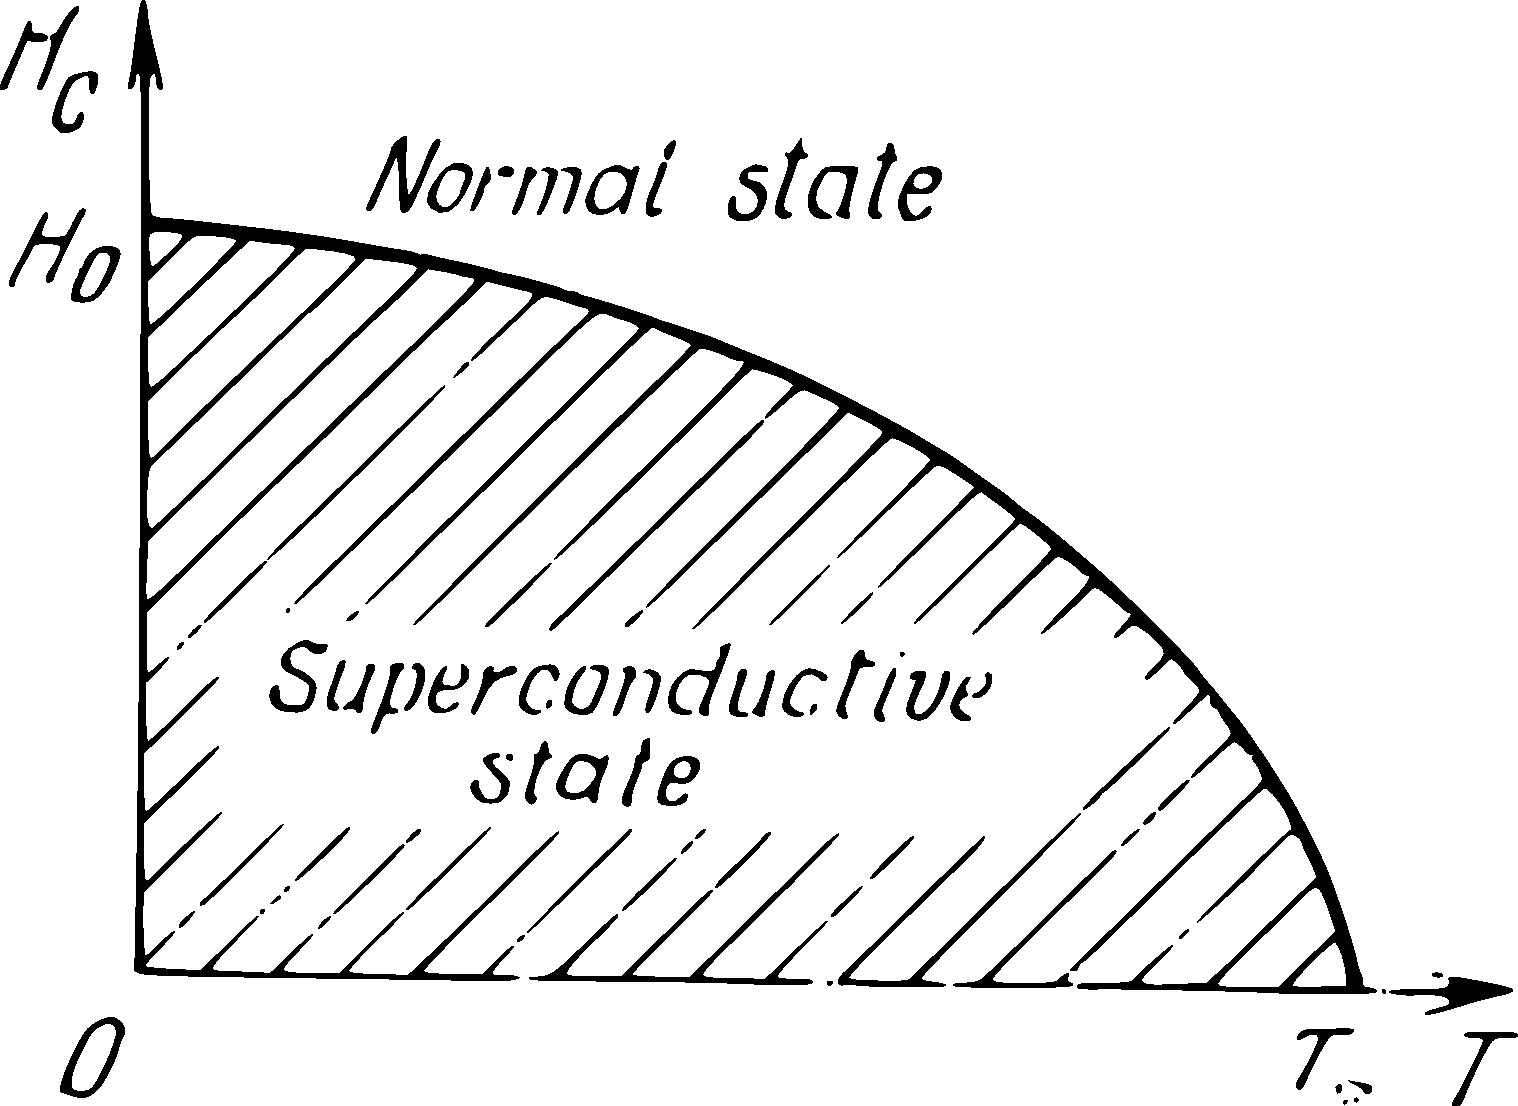
\includegraphics[width=\textwidth]{figs/ch-41/fig-41-07.pdf}
\sidecaption{The superconductive and normal states of a substance.\zhcap{物质的超导态与正常态。}\label{fig-41-07}}
\end{marginfigure}

\subsection{}\label{41.6.2} A sufficiently strong magnetic field at a given temperature destroys the superconductive state of a substance. When a magnetic field is applied to a superconductor, the transition temperature $T_{c}$ \ssect{41.6.1} is lowered.
\zhpar{在给定温度下，足够强的磁场会破坏物质的超导态。当对超导体施加磁场时，转变温度 $T_{c}$（\ssect{41.6.1}）会降低。}

A magnetic field of the strength $H_{c}$ which, at the given temperature, causes the transition of a substance from the superconductive to the normal state is called the \redem{critical field}. As the temperature of the superconductor is lowered, the field strength $H_{c}$ increases. As a first approximation: 
\zhpar{在给定温度下，能使物质由超导态转变为正常态的磁场强度 $H_{c}$ 称为\redem{临界磁场}。随着超导体温度降低，磁场强度 $H_{c}$ 增大。作为一级近似：}
\begin{equation*}%
H_{c} =  H_{0} \left[ 1 - \left( \frac{T}{T_{c}} \right)^{2} \right].
\end{equation*}
The curve in \figr{fig-41-07} separates the superconductive and normal states of a substance.
\zhpar{如\figr{fig-41-07}中的曲线所示，物质的超导态与正常态被该曲线分隔开来。}
\begin{marginfigure}[-1cm] 
\centering
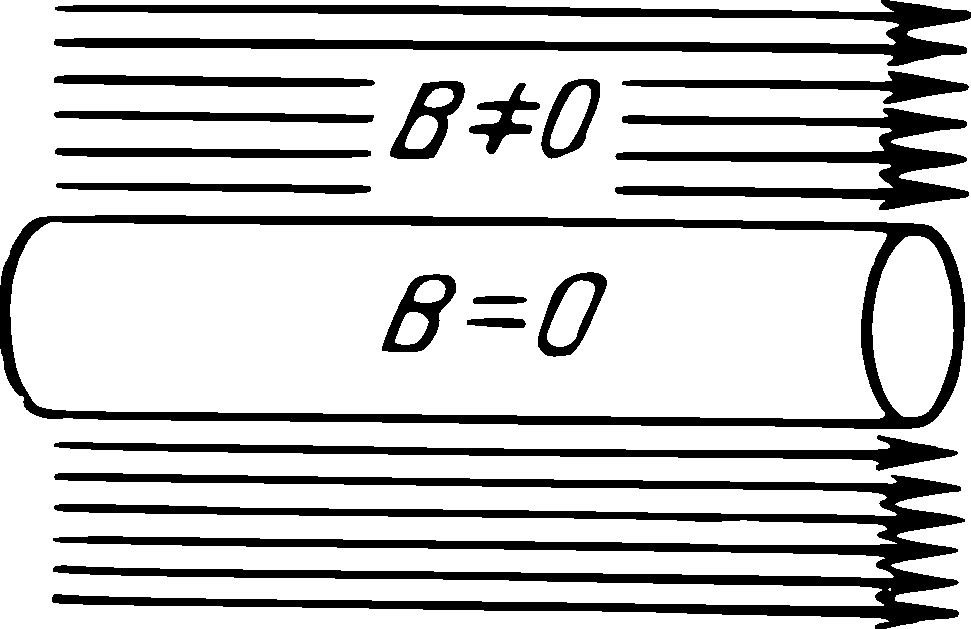
\includegraphics[width=0.8\textwidth]{figs/ch-41/fig-41-08.pdf}
\sidecaption{The external magnetic field weaker than the critical field does not penetrate interior of a superconductor.\zhcap{弱于临界磁场的外磁场不能穿入超导体内部。}\label{fig-41-08}}
\end{marginfigure}

The superconductive properties of a conductor disappear when
a sufficiently heavy current is passed through them. This is 
due to the action of the magnetic field, set up by the current, which destroys the superconductive state.
\zhpar{当通过导体的电流足够大时，导体的超导性质就会消失。这是由电流产生的磁场的作用所致，该磁场破坏了超导态。}



\subsection{}\label{41.6.3} An external magnetic field, weaker than the critical field \ssect{41.6.2} does not penetrate into the interior of a superconductor. Hence, the magnetic induction B \ssect{23.1.2} is always zero in the bulk of the superconductor. Shown in \figr{fig-41-08} is a uniform magnetic field \ssect{23.1.3} directed along the axis of a cylindrical superconductor. The superconductor seems to ``push'' the magnetic field out of the space it itself occupies and is an ideal diamagnetic material with a magnetic susceptibility of $\chi_{m} = -1$ \ssect{26.4.5}. Here the relative magnetic permeability $\mu_{r} = 1 + \chi_{m} = 0$ and $B = \mu_{0}\mu_{r}H = 0$.
\zhpar{弱于临界磁场（\ssect{41.6.2}）的外磁场不能穿入超导体内部。因此，超导体体内的磁感应强度 $B$（\ssect{23.1.2}）始终为零。如\figr{fig-41-08}所示，沿圆柱形超导体轴线方向的均匀磁场（\ssect{23.1.3}）被超导体“推出”其自身所占据的空间，超导体是一种磁化率为 $\chi_{m} = -1$ 的理想抗磁体（\ssect{26.4.5}）。此时相对磁导率 $\mu_{r} = 1 + \chi_{m} = 0$，且 $B = \mu_{0}\mu_{r}H = 0$。}

\begin{marginfigure}%[1cm] 
\centering
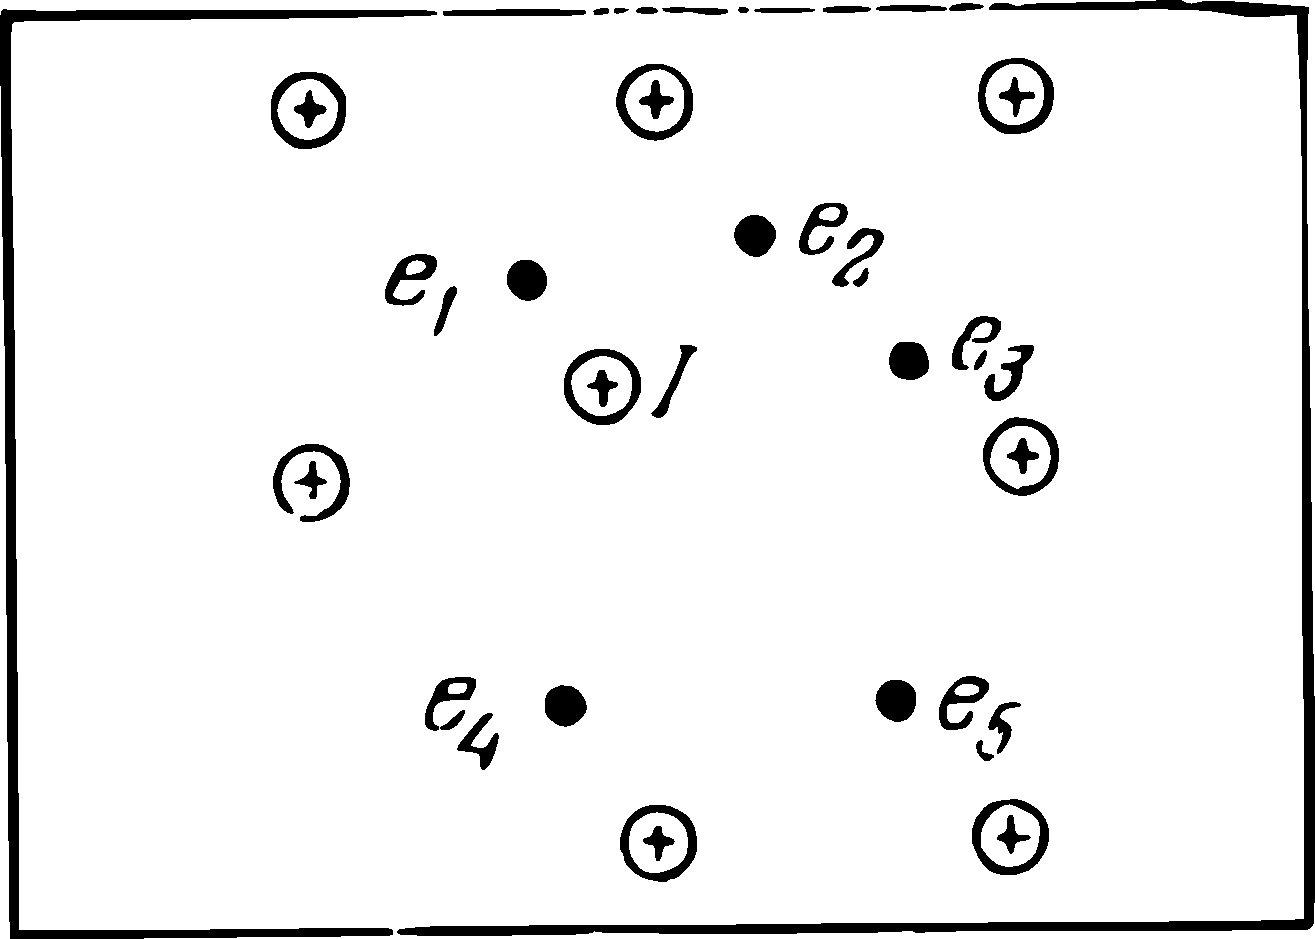
\includegraphics[width=\textwidth]{figs/ch-41/fig-41-09.pdf}
\sidecaption{A model of supercoductivity based on attraction between electrons and their pairing.\zhcap{基于电子间吸引及其成对的超导电性模型。}\label{fig-41-09}}
\end{marginfigure}
\subsection{}\label{41.6.4} The transition of a substance to the superconductive state is accompanied by changes in its thermal properties. In the absence of a magnetic field and at the transition temperature $T_{c}$ \ssect{41.6.1}, there is an abrupt change in the heat capacity \ssect{9.5.1}. In the presence of a magnetic field an isothermal transition from the superconductive to the normal state is associated with a jump in the heat conductivity and heat capacity. These phenomena are typical features of a second-order phase transition
\ssect{12.4.2}.
\zhpar{物质向超导态的转变伴随着热学性质的变化。在没有磁场、温度为转变温度 $T_{c}$（\ssect{41.6.1}）时，热容（\ssect{9.5.1}）发生突变。在有磁场的情况下，等温地由超导态转变为正常态时，热导率和热容都会出现跃变。这些现象是二级相变（\ssect{12.4.2}）的典型特征。}

\subsection{}\label{41.6.5} In quantum-mechanical theory, the phenomenon of superconductivity is considered to be the superfluidity \ssect{12.4.3} of electrons in a metal with the absence of friction inherent in superfluidity. The conduction electrons move along a superconductor unimpeded, i.e. without any ``friction'' between them and the crystal lattice points. The main feature of superconductors is that the mutual attraction of the electrons in them leads in the pairing of electrons. The cause of this attraction is interaction between electrons, supplementary to Coulomb repulsion, accomplished by the action of the crystal lattice and leading
in the pairing. 
\zhpar{在量子力学理论中，超导现象被看作金属中电子的超流动性（\ssect{12.4.3}），并且没有超流体固有的摩擦。导电电子沿超导体无阻地运动，即电子之间以及电子与晶格点之间没有任何“摩擦”。超导体的主要特征在于，其中电子之间的相互吸引导致电子成对。这种吸引力的起因是：除库仑斥力之外，电子之间还存在一种由晶格作用引起的相互作用，正是这种作用导致了电子成对。}




A model of this attraction is illustrated in \figr{fig-41-09}. Conduction electron $e_{1}$, attracts ion $I$ of the crystal
lattice to itself, displacing the ion from its equilibrium position. This changes the electric field in the crystal; ion $I$ sets up an electric field that acts on the conduction electrons, including electron $e_{2}$. Thus the interaction
between electrons $e_{1}$ and $e_{2}$ is accomplished by means of the crystal lattice. The displacement of the ion by an electron leads to a situation in which the electron is surrounded by a ``cloud'' of positive charge, which exceeds the intrinsic negative charge of the electron. Together with this ``cloud'' the electron has a net positive charge and is
thereby attracted to another electron.
\zhpar{这种吸引的模型如\figr{fig-41-09}所示。导电电子 $e_{1}$ 将晶格中的离子 $I$ 吸向自身，使离子偏离其平衡位置。这改变了晶体中的电场；离子 $I$ 产生的电场又作用于包括电子 $e_{2}$ 在内的导电电子。因此，电子 $e_{1}$ 与 $e_{2}$ 之间的相互作用是通过晶格实现的。电子使离子发生位移后，电子周围会形成一团正电荷“云”，其电量超过电子本身的负电荷。连同这团“云”，电子便带有净正电荷，从而被另一个电子所吸引。}

\subsection{}\label{41.6.6} In the quantum theory of metals attraction between electrons (phonon exchange) is associated with the setting up of elementary excitations (quasi-particles) of the crystal lattice. An electron, moving in a crystal and interacting with another electron by means of the lattice, brings the lattice into an excited state. As the lattice returns to the ground state it emits a quantum of energy of acoustic frequency, called a \redem{phonon} \ssect{41.7.5}, which is absorbed by the other electron. The attraction
between electrons can be conceived of as their exchange of
phonons. This attraction is found to be most effective if the
momenta of the interacting electrons are anti-parallel.
\zhpar{在金属的量子理论中，电子之间的吸引（声子交换）与晶格中基元激发（准粒子）的产生相联系。在晶体中运动的一个电子通过晶格与另一个电子相互作用，使晶格处于激发态。当晶格回到基态时，它发射出一个声频的能量量子，称为\redem{声子}（\ssect{41.7.5}），该声子被另一个电子吸收。电子之间的吸引可以理解为它们之间交换声子。研究发现，当相互作用的两个电子的动量反平行时，这种吸引最为有效。}

\subsection{}\label{41.6.7} The initiation of a superconductive state in a substance is associated with the possibility of forming bound pairs of electrons in the metal. The distance $\delta$ between the electrons of
a pair equals 
\zhpar{物质进入超导态与金属中形成束缚电子对的可能性有关。电子对中两电子之间的距离 $\delta$ 为：}
\begin{equation*}%
\delta = \frac{h \, u_{f}}{k T_{c}},
\end{equation*}
where $h$ is Planck's constant, $u_{F}$ is the velocity of an electron at the Fermi level \ssect{41.5.2}, $k$ is Boltzmann's constant \ssect{8.4.5}, and $T_{c}$ is the transition temperature to a superconductive state
\ssect{41.6.1}. An estimation indicates that $\delta \approx \SI{d-4}{\centi\meter}$, i.e. the electrons forming a pair are at a distance from each other of the order of \num{d4} crystal lattice constants. The whole electronic system of a superconductor is a bound aggregate extending over huge distances on the atomic scale.
\zhpar{式中 $h$ 为普朗克常量，$u_{F}$ 为费米能级上电子的速度（\ssect{41.5.2}），$k$ 为玻尔兹曼常量（\ssect{8.4.5}），$T_{c}$ 为向超导态转变的温度（\ssect{41.6.1}）。估算表明 $\delta \approx \SI{d-4}{\centi\meter}$，即组成电子对的两个电子之间的距离约为 $\num{d4}$ 个晶格常量的量级。超导体中的整个电子系统是一个在原子尺度上延伸到极大距离的束缚集合体。}

If at arbitrarily low temperatures Coulomb repulsion between
electrons predominates over the attraction that forms pairs,
the substance (metal or alloy) remains normal with respect to its electrical properties. But if the forces of attraction predominate over those of repulsion at the temperature $T_{c}$ \ssect{41.6.1}, the substance goes over to the superconductive state.
\zhpar{若在任意低的温度下，电子之间的库仑斥力都超过了形成电子对的吸引力，则该物质（金属或合金）的电学性质仍保持正常。但若在温度 $T_{c}$（\ssect{41.6.1}）时吸引力超过斥力，物质就会转变为超导态。}

\subsection{}\label{41.6.8} The most important feature associated with the pair in the aggregate of electrons in a superconductor is the impossibility of energy exchange between the electrons and the lattice in small portions, smaller than the binding energy of paired electrons. This means that in collisions between the electrons and the crystal lattice points, the energy of the electrons does not change, and the substance behaves as a superconductor with zero resistivity. A quantum-mechanical analysis shows that there is no scattering of electron waves by the thermal vibrations of the lattice or impurities. This is what indicates the absence of electrical resistance.
\zhpar{超导体中电子集合体里与电子对相关的最重要特征是：电子与晶格之间不可能以小于成对电子结合能的微小份额交换能量。这意味着在电子与晶格点碰撞时，电子的能量不发生改变，物质表现为电阻率为零的超导体。量子力学分析表明，晶格热振动和杂质都不会散射电子波，这正说明了电阻的不存在。}

\subsection{}\label{41.6.9} A definite amount of energy is required to destroy the state of superconductivity. At $T \gg T_{c}$ \ssect{41.6.1}, the bound states of the paired electrons are violated, attraction between the electrons ceases and superconductivity no longer exists.
\zhpar{破坏超导态需要一定的能量。当 $T \gg T_{c}$（\ssect{41.6.1}）时，成对电子的束缚态遭到破坏，电子之间的吸引作用消失，超导电性也不复存在。}

\subsection{}\label{41.6.10} Superconductivity is being used to produce strong magnetic fields because there are no thermal losses when heavy currents, required lo set up strong magnetic fields, are passed through superconductors. But, since a magnetic field destroys the state of superconductivity \ssect{41.6.2}, special \redem{type-$\mathit{2}$ superconductors} have been developed for obtaining strong magnetic fields. These are certain alloys and superconducting thin films.
\zhpar{由于超导体中通过产生强磁场所需的大电流时没有热损耗，超导性被用于产生强磁场。但是，由于磁场会破坏超导态（\ssect{41.6.2}），因此为获得强磁场，人们研制了特殊的\redem{第$\mathit{2}$类超导体}。它们是某些合金和超导薄膜。}

In such superconductors magnetic fields with a field strength
greater than $H_{c}$ \ssect{41.6.2} penetrate the substance in the form of threads piercing the specimen. The substance between the threads is found to be superconductive, and heavy currents can set up ultrastrong magnetic fields. Magnets, based on the application of superconducting solenoids, are being extensively used.
\zhpar{在这类超导体中，场强大于 $H_{c}$（\ssect{41.6.2}）的磁场以穿透样品的细丝（线）形式穿入物质。细丝之间的物质仍保持超导态，因此大电流可以产生超强磁场。基于超导螺线管的磁体目前已得到广泛应用。}

\section{Heat Capacity of Solids}
\label{sec-41.7} 
\zhtitle{固体的热容}


\subsection{}\label{41.7.1} No distinction is made for solids between the heat capacities $C_{v}$ and $C_{p}$ \ssect{9.5.4} and \ssect{9.5.7}. In nonmetallic solids, the largest contribution to heat capacity is made by the energy of thermal vibration of the particles at the crystal lattice points. For metals, a slight contribution is made by the degenerate electron gas \ssect{41.4.5}. 
\zhpar{对于固体，通常不区分定容热容 $C_{v}$ 与定压热容 $C_{p}$（\ssect{9.5.4}和\ssect{9.5.7}）。在非金属固体中，热容的最大贡献来自晶格格点上粒子的热振动能量。对于金属，简并电子气体也做出了较小的贡献（\ssect{41.4.5}）。}

\subsection{}\label{41.7.2} The classical theory of the heat capacity of solids /is based on the principle of equipartition of energy \ssect{10.6.4}. A homogeneous solid is dealt with as a system of particles, independent of one another, having three degrees of freedom and executing thermal vibrations with the same frequency. The
average energy $\expval{E}$ per degree of freedom is $\expval{E} = kT$ \ssect{10.6.5}. 
\zhpar{固体热容的经典理论以能量均分原理（\ssect{10.6.4}）为基础。均匀固体被看作由相互独立的粒子组成的系统，每个粒子具有三个自由度，并以相同频率做热振动。每个自由度的平均能量为 $\expval{E} = kT$（\ssect{10.6.5}）。}

The internal energy $U$ \ssect{9.1.2} per mole of a solid is
\zhpar{一摩尔固体的内能 $U$（\ssect{9.1.2}）为：}
\begin{equation*}%
U = 3 N_{A}\expval{E} = 3 N_{A}kT = 3 RT,
\end{equation*}
where $N_{A}$ is Avogadro's number (Appendix~II), $k$ is Boltzmann's constant \ssect{8.4.5}, and $R = kN_{A}$ is the universal gas constant \ssect{8.4.4}. The molar heat capacity \sidenote{Frequently, the heat capacity is referred to one gram-atom of the substance.} \ssect{9.5.4} of a solid with an atomic crystal lattice is
\zhpar{式中 $N_{A}$ 为阿伏伽德罗常量（附录II），$k$ 为玻尔兹曼常量（\ssect{8.4.5}），$R = kN_{A}$ 为摩尔气体常量（\ssect{8.4.4}）。具有原子晶格的固体的摩尔热容（\ssect{9.5.4}）为：}
\zhpar{注：热容常以物质的一克原子为单位来表示。}
\begin{equation*}%
C_{\mu} = \pdv{U}{T} = 3 R = \SI{25}{\joule\per\mole\per\kelvin} = \SI{25}{\calorie\per\mole\per\kelvin},
\end{equation*}
The \redem{Dulong-Petit law} states that the molar heat capacity of all chemically simple crystalline solids equals approximately \SI{6}{\calorie\per\mole\per\kelvin}. According to this law tha molar heat capacity does not depend on either the temperature or any characteristics of the crystals. 
\zhpar{\redem{杜隆-珀蒂定律}指出，所有化学成分简单的结晶固体的摩尔热容约等于 \SI{6}{\calorie\per\mole\per\kelvin}。根据该定律，摩尔热容既不依赖于温度，也不依赖于晶体的任何特性。}

\begin{marginfigure}%[1cm] 
\centering
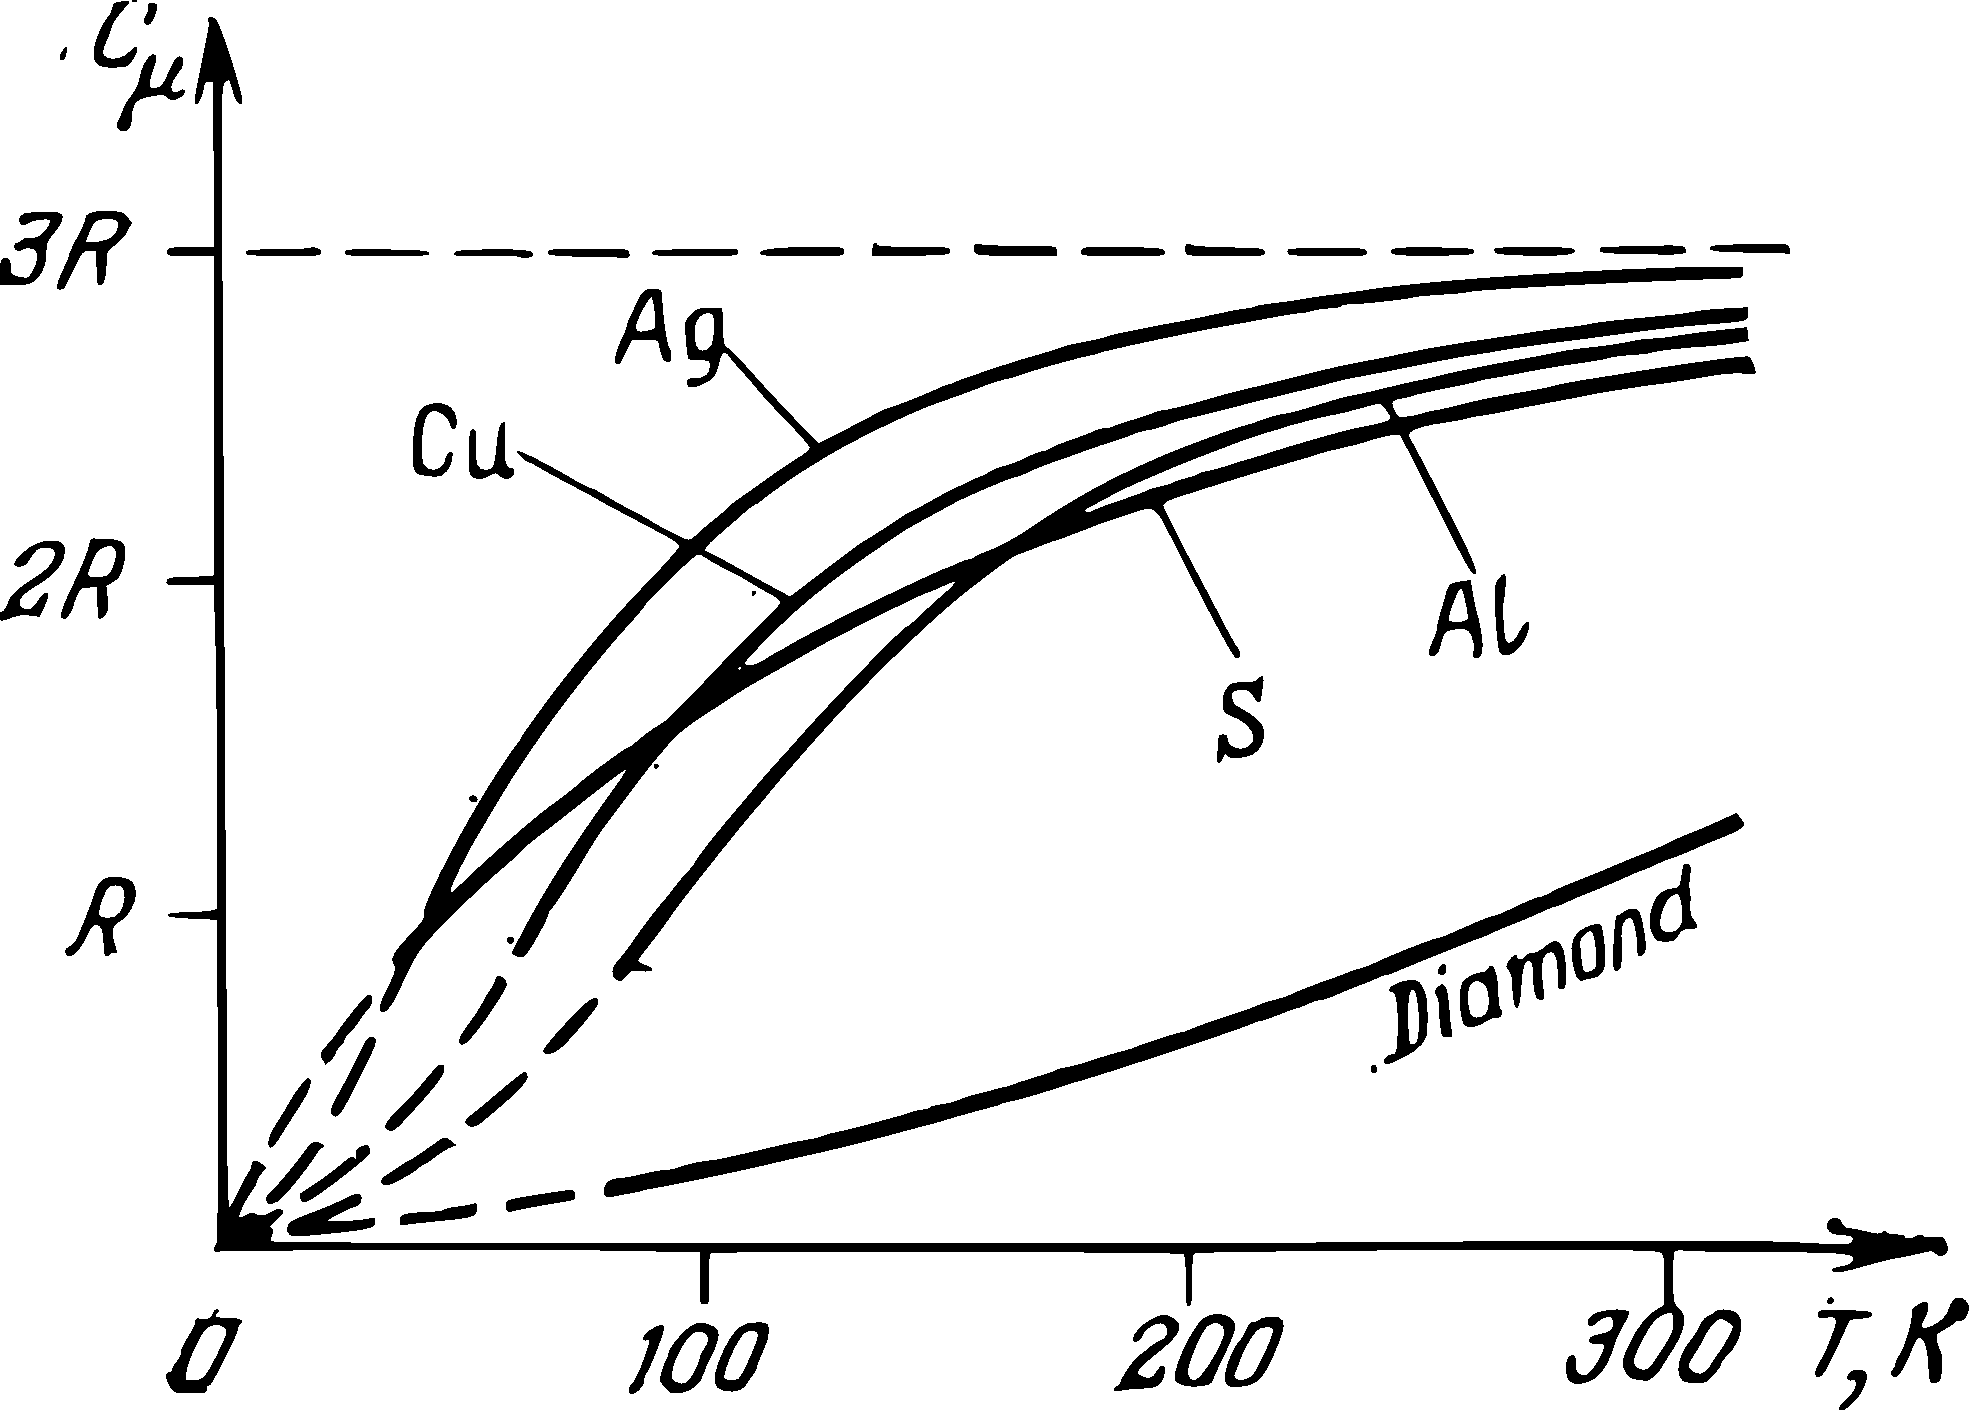
\includegraphics[width=\textwidth]{figs/ch-41/fig-41-10.pdf}
\sidecaption{Heat capacity as a function of temperature.\zhcap{热容随温度的变化。}\label{fig-41-10}}
\end{marginfigure}


Experiments disprove this statement and indicate that the heat capacity depends on the temperature, especially  in the region of low temperatures (\figr{fig-41-10}). The reason why t he classical theory of the heat capacity of solids disagrees with experimental data is in the limited nature of the principle of equipartition of energy and its inadequacy in the region of low temperatures. At these temperatures the average energy of the vibrating particles must be calculated in accordance with the laws of quantum mechanics \ssect{38.5.9}.
\zhpar{实验否定了这一说法，表明热容随温度变化，尤其在低温区域（见\figr{fig-41-10}）。经典固体热容理论与实验数据不符的原因在于能量均分原理具有局限性，它在低温区域并不适用。在这些温度下，振动粒子的平均能量必须按照量子力学规律计算（\ssect{38.5.9}）。}


\subsection{}\label{41.7.3} In the initial quantum theory of heat capacity of solids, a crystal was treated as a system of $N$ atoms, each of which is a quantum harmonic oscillator. All the atoms vibrate independently of one another with the same frequency $\omega$. The average energy $\expval{E}$ per degree of freedom of the atom (as a quantum harmonic oscillator) is equal \ssect{38.5.9} to
\zhpar{在固体热容的早期量子理论中，晶体被看作由 $N$ 个原子组成的系统，每个原子都是一个量子谐振子。所有原子以相同的频率 $\omega$ 彼此独立地振动。作为量子谐振子，原子每个自由度的平均能量等于（\ssect{38.5.9}）：}
\begin{equation*}%
\expval{E} = \frac{\hbar \omega}{\exp (\hbar \omega/kT) - 1}
= \frac{h \nu}{\exp (h \nu /kT) - 1},
\end{equation*}
The internal energy $U$ \ssect{9.1.2} of a mole of a solid is expressed as follows:
\zhpar{一摩尔固体的内能 $U$（\ssect{9.1.2}）可表示为：}
\begin{equation*}%
U = 3 N_{A} \expval{E} = 3 N_{A} \frac{h \nu}{\exp (h \nu /kT) - 1},
\end{equation*}
from which the molar heat capacity of a solid can be found
\zhpar{由此可求得固体的摩尔热容为：}
\begin{equation*}%
C_{\mu} = 3 R \left( \frac{h \nu}{kT} \right)^{2} = \frac{\exp (h \nu /kT)}{[\exp (h \nu /kT) - 1]^{2}}
\end{equation*}
If we introduce the \redem{characteristic temperature} $T_{\theta} = h\nu/kT$, then 
\zhpar{若引入\redem{特征温度} $T_{\theta} = h\nu/kT$，则有：}
\begin{equation*}%
C_{\mu} = 3 R \left( \frac{T_{\theta}}{T} \right)^{2} = \frac{\exp (T_{\theta}/T)}{[\exp (T_{\theta}/T) - 1]^{2}}.
\end{equation*}
This result, qualitatively describes the dependence of the heat capacity of solids on the temperature. Curves of this dependence are plotted in \figr{fig-41-10}.
\zhpar{这一结果定性地描述了固体热容随温度的变化，该变化关系的曲线见\figr{fig-41-10}。}

At high temperatures $(h \nu \ll kT)$, as shown in \ssect{38.5.9}, $\expval{E}  = kT$ in accordance with the law of equipartition of energy \ssect{10.6.4} and $C_{\mu} = 3R$.
\zhpar{在高温（$h \nu \ll kT$）下，如\ssect{38.5.9}所示，$\expval{E} = kT$，符合能量均分原理（\ssect{10.6.4}），且 $C_{\mu} = 3R$。}

At low temperatures $(h \nu \gg kT)$, hence $\exp (h \nu /kT) - 1 \approx \exp (h \nu /kT)$ and
\zhpar{在低温（$h \nu \gg kT$）下，因此 $\exp (h \nu /kT) - 1 \approx \exp (h \nu /kT)$，且有：}
\begin{equation*}%
C_{\mu} = 3 R \left( \frac{T_{\theta}}{T} \right)^{2}  \exp (-T_{\theta}/T).
\end{equation*}
As $T \to 0$, $T_{\theta}/T \to \infty$ and $\exp (- T_{\theta}/T) \to 0$ more rapidly than the increase in $(T_{\theta}/T)^{2}$. Therefore, as $T \to 0$, the heat
capacity $C_{\mu} \to 0$. This qualitatively agrees with experimental data. But simple quantum theory does not explain the quantitative behaviour of solids in the vicinity of absolute zero.
\zhpar{当 $T \to 0$ 时，$T_{\theta}/T \to \infty$，且 $\exp (- T_{\theta}/T) \to 0$ 的速度快于 $(T_{\theta}/T)^{2}$ 的增长速度。因此，当 $T \to 0$ 时，热容 $C_{\mu} \to 0$。这与实验数据定性相符，但简单的量子理论无法解释固体在绝对零度附近的定量行为。}

\subsection{}\label{41.7.4} The assumption that all the atoms of a solid execute thermal vibrations independently of one anotheiat the same frequency oversimplifies the true picture of particle vibration in a crystal lattice. The interaction between the atoms (or other particles) of a solid is so strong that all $N$ particles of the body form a bound system having $3N$ degrees of freedom, and the vibration of all the atoms may proceed at various frequencies.
\zhpar{假定固体中所有原子以相同频率彼此独立地做热振动，过分简化了晶格中粒子振动的真实图像。固体中原子（或其他粒子）之间的相互作用非常强，以至于物体中全部 $N$ 个粒子构成一个具有 $3N$ 个自由度的束缚系统，所有原子的振动可以以各种不同的频率进行。}

The extremely complex problem of the frequency distribution
of atomic vibration in a solid was, in its time, the basis for the refined theory of heat capacity of solids. A solid has a wide spectrum of vibrational frequencies. There are vibrations with sufficiently low and with higher frequencies. The low frequencies correspond to elastic vibration of the crystal in the acoustic (or ultrasonic) range. Owing to the bonds between the particles of a crystal lattice, elastic acoustic waves propagate in the crystal.
\zhpar{在当时，固体中原子振动频率分布这一极为复杂的问题，是改进的固体热容理论的基础。固体具有宽广的振动频谱，既有较低频率的振动，也有较高频率的振动。低频振动对应于晶体在声频（或超声频）范围内的弹性振动。由于晶格中粒子之间存在键合，弹性声波可以在晶体中传播。}

The physical idea of the theory of the heat capacity of solids, refining the theory discussed in \ssect{41.7.3}, is that the main contribution to the energy of thermal vibration of the crystal is made by low-frequency vibration, corresponding to elastic waves with wavelengths, exceeding the crystal lattice constant.
\zhpar{对\ssect{41.7.3}中的理论加以改进后，固体热容理论的物理思想是：晶体热振动能量的主要贡献来自低频振动，即波长大于晶格常量的弹性波。}

This follows, in particular, from \figr{fig-38-07}, which shows that the maximum contribution to the average energy of a quantum oscillator is made by vibrations with low frequencies \ssect{38.5.9}.
\zhpar{由\figr{fig-38-07}可以特别看出这一点，该图表明，量子振子平均能量的最大贡献来自低频振动（\ssect{38.5.9}）。}

The propagating elastic waves behave as if they were propagating in a continuous medium. The atomic structure of the crystal has no effect on the propagation in it of elastic waves of wavelengths exceeding $\lambda_{min} = v / \lambda_{max}$, where $v$ is the velocity of the corresponding elastic wave, and vmax is its frequency. The wavelength $\lambda_{min}$ should be commensurable with the lattice constant, i.e. i $\lambda_{min} \approx d \approx (V/N)^{1/3}$, where $N$ is the number of particles (crystal lattice points) in a crystal of volume $V$.
\zhpar{传播中的弹性波表现得仿佛是在连续介质中传播。对于波长大于 $\lambda_{min} = v / \lambda_{max}$ 的弹性波（式中 $v$ 为相应弹性波的速度，$\nu_{\max}$ 为其频率），晶体的原子结构对其传播没有影响。波长 $\lambda_{min}$ 应与晶格常量处于同一数量级，即 $\lambda_{min} \approx d \approx (V/N)^{1/3}$，式中 $N$ 为体积为 $V$ 的晶体中的粒子（晶格格点）数。}

\subsection{}\label{41.7.5} Elastic waves in a crystal have quantum properties consisting in the existence of a minimum portion of energy, a quantum of energy of the wave with the given frequency $\nu$. This enables a wave with the frequency $\nu$ to be correlated to a \redem{quasi-particle}, the \redem{phonon}, whose propagation at the velocity of sound $v$ corresponds to an acoustic wave.
\zhpar{晶体中的弹性波具有量子性质，即存在最小的能量份额，即频率为 $\nu$ 的波的能量量子。这使得频率为 $\nu$ 的波可以与一种\redem{准粒子}——\redem{声子}相对应，其以声速 $v$ 传播，对应于一个声波。}

A phonon has the energy $E = h\nu$, where $h$ is Planck's constant (Appendix~II), and the quasi-momentum $p = h\nu /v$. The \redem{quasimomentum $\vb{p}$ of the phonon} is in the direction coinciding with that of the propagation of the acoustic wave. The most essential difference between the quasi-momentum and the momentum is that in the collision of phonons in crystals the quasi-momentum can be transferred in discrete portions to the crystal lattice. In this case it is not conserved.\sidenote{A detailed discussion of the properties of quasi-particles, associated with the role of periodicity of crystal structure, is beyond the scope of this handbook.} 
\zhpar{声子的能量为 $E = h\nu$，其中 $h$ 为普朗克常量（附录II），其准动量为 $p = h\nu /v$。声子的\redem{准动量} $\vb{p}$ 的方向与声波的传播方向一致。准动量与动量最本质的区别在于：在晶体中声子碰撞时，准动量可以以分立的份额传递给晶格，因此准动量不守恒。}
\zhpar{注：关于准粒子的性质及其与晶体结构周期性之间关系的详细讨论，超出了本手册的范围。}

In short, the quantization of the acoustic field leads to phonons in the same way as the quantization of the electromagnetic field leads to photons \ssect{37.1.4}.
\zhpar{简言之，声场的量子化导致声子的产生，正如电磁场的量子化导致光子的产生一样（\ssect{37.1.4}）。}

\subsection{}\label{41.7.6} Phonon spin equals zero and, therefore, phonons comply with Bose-Einstein statistics \ssect{41.2.2}. Phonons can be emitted and they can be absorbed, but their number is not maintained constant, hence the chemical potential for phonon gas \ssect{41.2.3}
equals zero (cf. \ssect{41.2.6}). 
\zhpar{声子的自旋为零，因此声子遵从玻色-爱因斯坦统计（\ssect{41.2.2}）。声子可以被发射，也可以被吸收，其数目并不保持恒定，因此声子气体的化学势（\ssect{41.2.3}）等于零（参见\ssect{41.2.6}）。}

The energy of a crystal can be dealt with as the energy of a phonon gas and can be calculated as in \ssect{41.2.6}. The number $\dd N$ of phonons with frequencies in the range from $\nu$ to $\nu + \dd \nu$ is
\zhpar{晶体的能量可以当作声子气体的能量来处理，并可按照\ssect{41.2.6}中的方法进行计算。频率在 $\nu$ 到 $\nu + \dd \nu$ 范围内的声子数 $\dd N$ 为：}
\begin{equation*}%
\dd N = \frac{\dd g}{\exp (h \nu/k T)-1},
\end{equation*}
where $\dd g$ is the number of quantum states (number of cells) in volume $V$ of the crystal:
\zhpar{式中 $\dd g$ 为晶体体积 $V$ 中的量子态数（即格子数）：}
\begin{equation*}%
\dd g = 3 \frac{4 \pi p^{2} \dd p \, V}{h^{3}} = 3 \frac{4 \pi \nu^{2} \dd \nu}{v^{3}} V,
\end{equation*}
where $p = h\nu/v$ is the quasi-momentum of the phonon, and $v$ is the velocity of sound in the crystal. The factor 3 takes into account the fact that longitudinal and transverse waves, with two mutually perpendicular polarizations, can propagate in a crystal\sidenote{The difference in the velocities of the longitudinal and transverse waves is ignored, the number of quantum states of the phonons being simply tripled.} \ssect{31.1.8}. Thus
\zhpar{式中 $p = h\nu/v$ 为声子的准动量，$v$ 为晶体中的声速。因子 3 考虑了晶体中纵波与横波都可以传播这一事实，纵波与横波具有两个相互垂直的偏振方向（\ssect{31.1.8}）。由此有：}
\zhpar{注：此处忽略了纵波与横波速度的差别，声子的量子态数被简单地乘以 3。}
\begin{equation*}%
\dd N = \frac{12 \pi \nu^{2} \dd \nu \, V}{v^{3}(\exp (h \nu/k T)-1)}.
\end{equation*}
The internal energy $U$ \ssect{9.1.2} of a crystal (accurate to zero-point energy) is
\zhpar{晶体的内能 $U$（\ssect{9.1.2}）（精确到零点能）为：}
\begin{equation*}%
U = \int_{0}^{\nu_{max}}h \nu \dd N = \frac{12 \pi  Vh}{v^{3}} 
\int_{0}^{\nu_{max}} \frac{\nu^{3} \dd \nu}{\exp (h \nu/k T)-1},
\end{equation*}
where $\nu_{max} = v (3N/4 \pi V)^{1/3}$ is the upper frequency boundary of the phonons that contribute to the energy of/tfiermat vibration of the crystal. An assessment of the order of magnitude of $\nu_{max}$ is given in \ssect{41.7.4}.
\zhpar{式中 $\nu_{max} = v (3N/4 \pi V)^{1/3}$ 为对晶体热振动能量有贡献的声子的频率上限。关于 $\nu_{max}$ 的数量级估计见\ssect{41.7.4}。}

Introduced in calculating $U$ is the \redem{Debye characteristic temperature} $T_{D} = h\nu_{max}/k$. The following two limiting cases are considered.
\zhpar{在计算 $U$ 时引入了\redem{德拜特征温度} $T_{D} = h\nu_{max}/k$。下面考虑两种极限情形。}
\begin{enumerate}[label = (\alph*)]
\item \emph{High temperatures $T \gg T_{D}$.}
\zhpar{\emph{高温情形 $T \gg T_{D}$。}}

Here $\exp h\nu / kT - 1 \approx \frac{h\nu}{kT}$, and 
\zhpar{此时 $\exp h\nu / kT - 1 \approx \frac{h\nu}{kT}$，于是有：}
\begin{equation*}%
U = \frac{12 \pi V}{v^{3}} kT \int_{0}^{\nu_{max}} \nu^{2} \dd \nu = \frac{12\pi V kT}{v^{3}}  \, \frac{\nu_{max}^{3}}{3} = 3 NkT.
\end{equation*}
For one mole of the crystal $N = N_{A}$ where $N$ is Avogadro's number (Appendix~II), and the molar heat capacity $C_{\mu}$ complies with the Dulong-Petit law \ssect{41.7.2}:
\zhpar{对于一摩尔晶体，$N = N_{A}$（式中 $N_{A}$ 为阿伏伽德罗常量，附录II），摩尔热容 $C_{\mu}$ 遵从杜隆-珀蒂定律（\ssect{41.7.2}）：}
\begin{equation*}%
C_{\mu} = \pdv{U}{T} = 3 N_{A} k=3R.
\end{equation*}
\item \emph{Low temperatures $T \ll T_{D}$.}
In calculating the integral $\int_{0}^{\nu_{max}} \frac{\nu^{3} \dd \nu}{\exp (h \nu/k T)-1}$, a new variable $\xi = \exp (h \nu/k T)$, is introduced and the upper limit is
replaced by $\infty$. Thus
\zhpar{\emph{低温情形 $T \ll T_{D}$。}在计算积分 $\int_{0}^{\nu_{max}} \frac{\nu^{3} \dd \nu}{\exp (h \nu/k T)-1}$ 时，引入新变量 $\xi = \exp (h \nu/k T)$，并将积分上限替换为 $\infty$。由此有：}
\begin{align*}%
U & = \frac{12 \pi Vh}{v^{3}} \int_{0}^{\nu_{max}} \frac{\nu^{3} \dd \nu}{\exp (h \nu/k T)-1}\\
& = \frac{12 \pi V h}{v^{3}}  \left( \frac{kT}{h}\right)^{4} \int_{0}^{\infty} \frac{\xi^{3} \dd \xi}{\exp \xi - 1}\\
& = \frac{4 \pi^{4}k^{4}V}{5h^{3}v^{3}} T^{4}.
\end{align*}
The molar heat capacity is proportional to the cube of the absolute temperature and obeys the \redem{Debye $T^{3}$ law}. Thus 
\zhpar{摩尔热容与热力学温度的三次方成正比，遵从\redem{德拜 $T^{3}$ 定律}。由此有：}
\begin{equation*}%
C_{\mu} = \pdv{U}{T} = \frac{16\pi^{5}k^{4}V T^{3}}{5 h^{3}v^{3}} = \text{const } T^{3}.
\end{equation*}

\end{enumerate}

\section{Band Theory of Solids}
\label{sec-41.8} 
\zhtitle{固体的能带理论}

\subsection{}\label{41.8.1} Long-range order in crystals \ssect{40.1.1} leads to a situation in which an electric field, which is a periodic function of the coordinates, exists in solids. In a metal, for example, where the positive ions are located in strict order at the lattice points, the potential energy of an electron varies along some direction
$OX$ as shown in \figr{fig-41-11}. Energy minima correspond to the places where the positive ions are located.
\zhpar{晶体中的长程有序（\ssect{40.1.1}）使固体中存在一个坐标的周期函数形式的电场。例如在金属中，正离子严格有序地位于格点上，电子的势能沿某一方向 $OX$ 变化，如\figr{fig-41-11}所示。势能极小值对应于正离子所在的位置。}

\begin{marginfigure}%[1cm] 
\centering
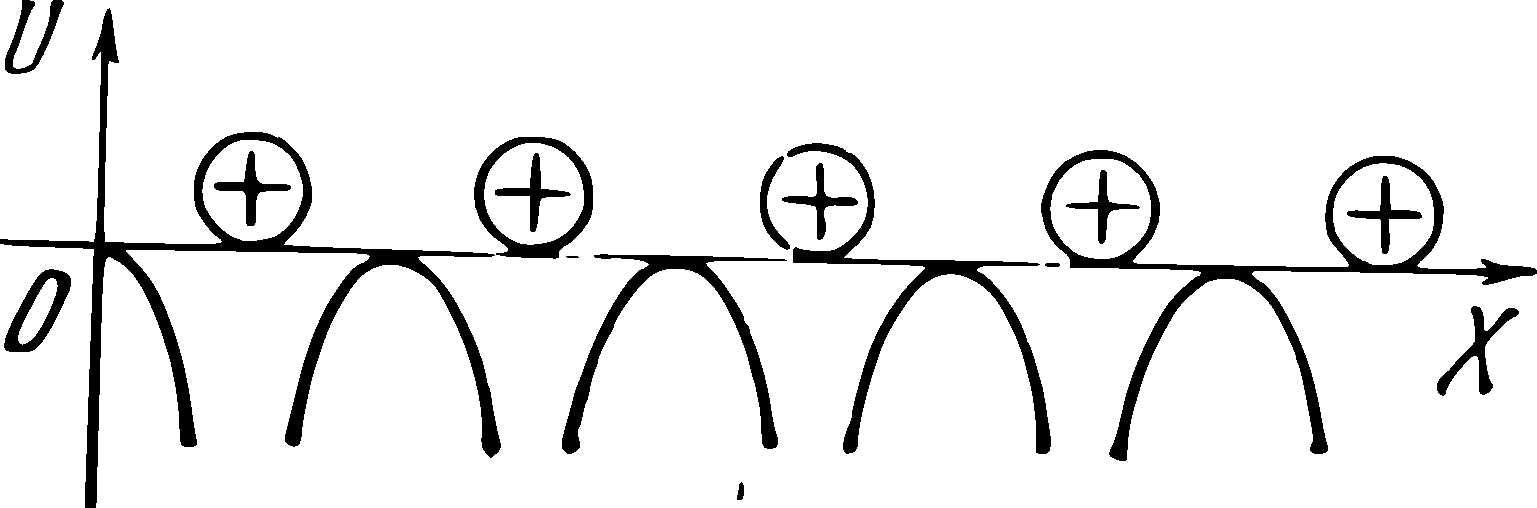
\includegraphics[width=\textwidth]{figs/ch-41/fig-41-11.pdf}
\sidecaption{Energy in a lattice is dependent on the position of ions. \zhcap{晶格中的能量取决于离子的位置。}\label{fig-41-11}}
\end{marginfigure}

\subsection{}\label{41.8.2} A periodic electric field in a crystal of any type \ssect{40.1.3} essentially changes the energy states of the electrons in a solid as compared to their state in single atoms. In single atoms the electrons are in discrete energy states \ssect{38.2.5}. In a solid, the energy states of the electrons are determined both by their interaction with the nucleus of their atom and by the electric Held of the crystal lattice, i.e. by their interaction with other atoms. 
\zhpar{任何类型晶体中的周期性电场（\ssect{40.1.3}），都使固体中电子的能量状态与单个原子中的状态相比发生了根本性的改变。在单个原子中，电子处于分立的能态（\ssect{38.2.5}）。在固体中，电子的能态既由其与所在原子核的相互作用决定，也由晶格的电场决定，即由其与其他原子的相互作用决定。}

As a result of this interaction, the energy levels of the electrons are split. Thus, in a solid containing $N$ interacting atoms, $N$ closely spaced energy levels are formed in place of the discrete energy level typical of a single atom. These $N$ energy levels make up an \redem{energy band}. A \redem{band energy spectrum of the electrons} is formed in crystals.
\zhpar{由于这种相互作用，电子的能级发生分裂。因此，在包含 $N$ 个相互作用原子的固体中，原来单个原子中的一个分立能级，被 $N$ 个间距很小的能级所取代。这 $N$ 个能级构成一个\redem{能带}。晶体中形成了电子的\redem{能带谱}。}

\subsection{}\label{41.8.3} The, formation of a band energy spectrum in a crystal follows from the indeterminacy principle \ssect{38.6.6}. Owing to the finite lifetime $\tau$ of the electron in an excited state $(\tau \approx \SI{d-8}{\second})$ \ssect{39.1.5} the width $\Delta E$ of the energy level in a single atom is
\zhpar{晶体中能带谱的形成源于不确定关系（\ssect{38.6.6}）。由于电子在激发态中的寿命 $\tau$ 有限（$\tau \approx \SI{d-8}{\second}$，\ssect{39.1.5}），单个原子中能级的宽度 $\Delta E$ 为：}
\begin{equation*}%
\Delta E \approx \frac{\hbar}{\tau} = \approx \SI{d-7}{\electronvolt},
\end{equation*}
(\redem{natural} energy level \redem{width}).
\zhpar{（\redem{自然}能级\redem{宽度}）。}

The valence electrons \ssect{39.3.9} of the atoms in a crystal are more weakly bound to the nuclei than the inner-shell electrons and can pass from one atom to another by means of the tunnel effect \ssect{38.7.2}. In this way electrons penetrate the potential barrier \ssect{38.7.1} separating the atoms of the crystal.
\zhpar{晶体中原子的价电子（\ssect{39.3.9}）与原子核的束缚比内层电子弱，可以借助隧道效应（\ssect{38.7.2}）从一个原子转移到另一个原子。电子就是以这种方式穿透分隔晶体中各原子的势垒（\ssect{38.7.1}）的。}

To assess the average lifetime x of a valence electron in a given atom it is assumed that the penetrability $D$ of the barrier is expressed by the simple formula \ssect{38.7.2}
\zhpar{为估算给定原子中价电子的平均寿命 $\tau$，假定势垒的穿透系数 $D$ 可由下面的简单公式表示（\ssect{38.7.2}）：}
\begin{equation*}%
D \approx \exp \left( -\frac{2}{\hbar} \sqrt{2m(U_{0}- E) } L \right),
\end{equation*}
where $U_{0} - E$ is the barrier height, consisting of the ionization energy, and amounts to approximately \approx \SI{10}{\electronvolt}, and $L$ is the barrier width, which is commensurate with the crystal lattice constant: $L \approx  d \approx \SI{d-10}{\meter}$. The frequency $\nu$ of penetration of an electron through the barrier is
\zhpar{式中 $U_{0} - E$ 为势垒高度，由电离能构成，约为 $\approx \SI{10}{\electronvolt}$；$L$ 为势垒宽度，与晶格常量处于同一数量级：$L \approx  d \approx \SI{d-10}{\meter}$。电子穿透势垒的频率 $\nu$ 为：}
\begin{equation*}%
\nu  = \frac{v}{d} D \approx \frac{v}{d} \exp \left( -\frac{2}{\hbar} \sqrt{2m(U_{0}- E) } L \right),
\end{equation*}
where $v$ is the velocity of the electron in the atom (potential well) and can be taken equal to $v = \SI{d6}{\meter\per\second}$. The average lifetime $\tau$ of an electron in the given atom is 
\zhpar{式中 $v$ 为电子在原子中（势阱中）的速度，可取 $v = \SI{d6}{\meter\per\second}$。电子在给定原子中的平均寿命 $\tau$ 为：}
\begin{equation*}%
\tau  = \frac{1}{\nu}  \approx \frac{d}{v} \exp \left(\frac{2}{\hbar} \sqrt{2m(U_{0}- E) } L \right).
\end{equation*}
After substituting the values of all the quantities, $\tau = \SI{d-15}{\second}$ is obtained. From the indeterminacy relation
\zhpar{代入各量的数值后，得到 $\tau = \SI{d-15}{\second}$。由不确定关系可得：}
\begin{equation*}%
\Delta E \approx \frac{\hbar}{\tau} \approx \SI{1}{\electronvolt}
\end{equation*}
Instead of the natural width $\Delta E \approx \SI{d-7}{\electronvolt}$ of the electron energy level in a single atom, a band of allowed values of energy is formed in a crystal.
\zhpar{与单个原子中电子能级的自然宽度 $\Delta E \approx \SI{d-7}{\electronvolt}$ 不同，晶体中形成了由允许能量值构成的能带。}

\subsection{}\label{41.8.4} The frequency of the penetration of inner-shell electrons in atoms through a potential barrier and their transitions to other atoms is negligible. This is due to the increase in barrier height: $U_{0} - E \approx \SI{d3}{\electronvolt}$ and the increase in barrier width:
$L \approx \SI{3d-10}{\meter}$. According to calculations, $\tau \approx \num{d20}$ years. The broadening of the energy levels of the inner-shell electrons is unessential, and these electrons behave in crystals practically in the same way as in single atoms.
\zhpar{内层电子穿过势垒进入相邻原子并发生跃迁的频率可以忽略不计。这是因为势垒高度增大为 $U_{0} - E \approx \SI{d3}{\electronvolt}$，势垒宽度增大为 $L \approx \SI{3d-10}{\meter}$。据计算，$\tau \approx \num{d20}$ 年。内层电子能级的展宽并不重要，这些电子在晶体中的行为与在单个原子中的行为基本相同。}

\subsection{}\label{41.8.5} If $N$ is the total number of atoms in a solid, then the energy band, formed from the electronic energy level of the valence electron of the atom consists of N closely spaced levels. Adjacent energy levels in a band are at about $\SI{d-22}{\electronvolt}$ from each
other.
\zhpar{若 $N$ 为固体中的原子总数，则由原子价电子能级形成的能带由 $N$ 个间距很小的能级组成。能带中相邻能级之间的间距约为 $\SI{d-22}{\electronvolt}$。}

The allowed energy bands are separated by regions that are
\redem{forbidden bands} of electron energy values. The width of the forhidden bands is commensurable with that of the allowed bands. With an increase in energy the width of the allowed energy hands increases and that of the forbidden bands decreases. A schematic diagram of the energy bands of a solid is shown in \figr{fig-41-12}.
\zhpar{允许能带之间的区域是\redem{禁带}，即电子能量值不允许取的区域。禁带宽度与允许能带宽度为同一数量级。随着能量增大，允许能带的宽度增大，而禁带的宽度减小。固体能带的示意图如\figr{fig-41-12}所示。}

\begin{figure}%[1cm] 
\centering
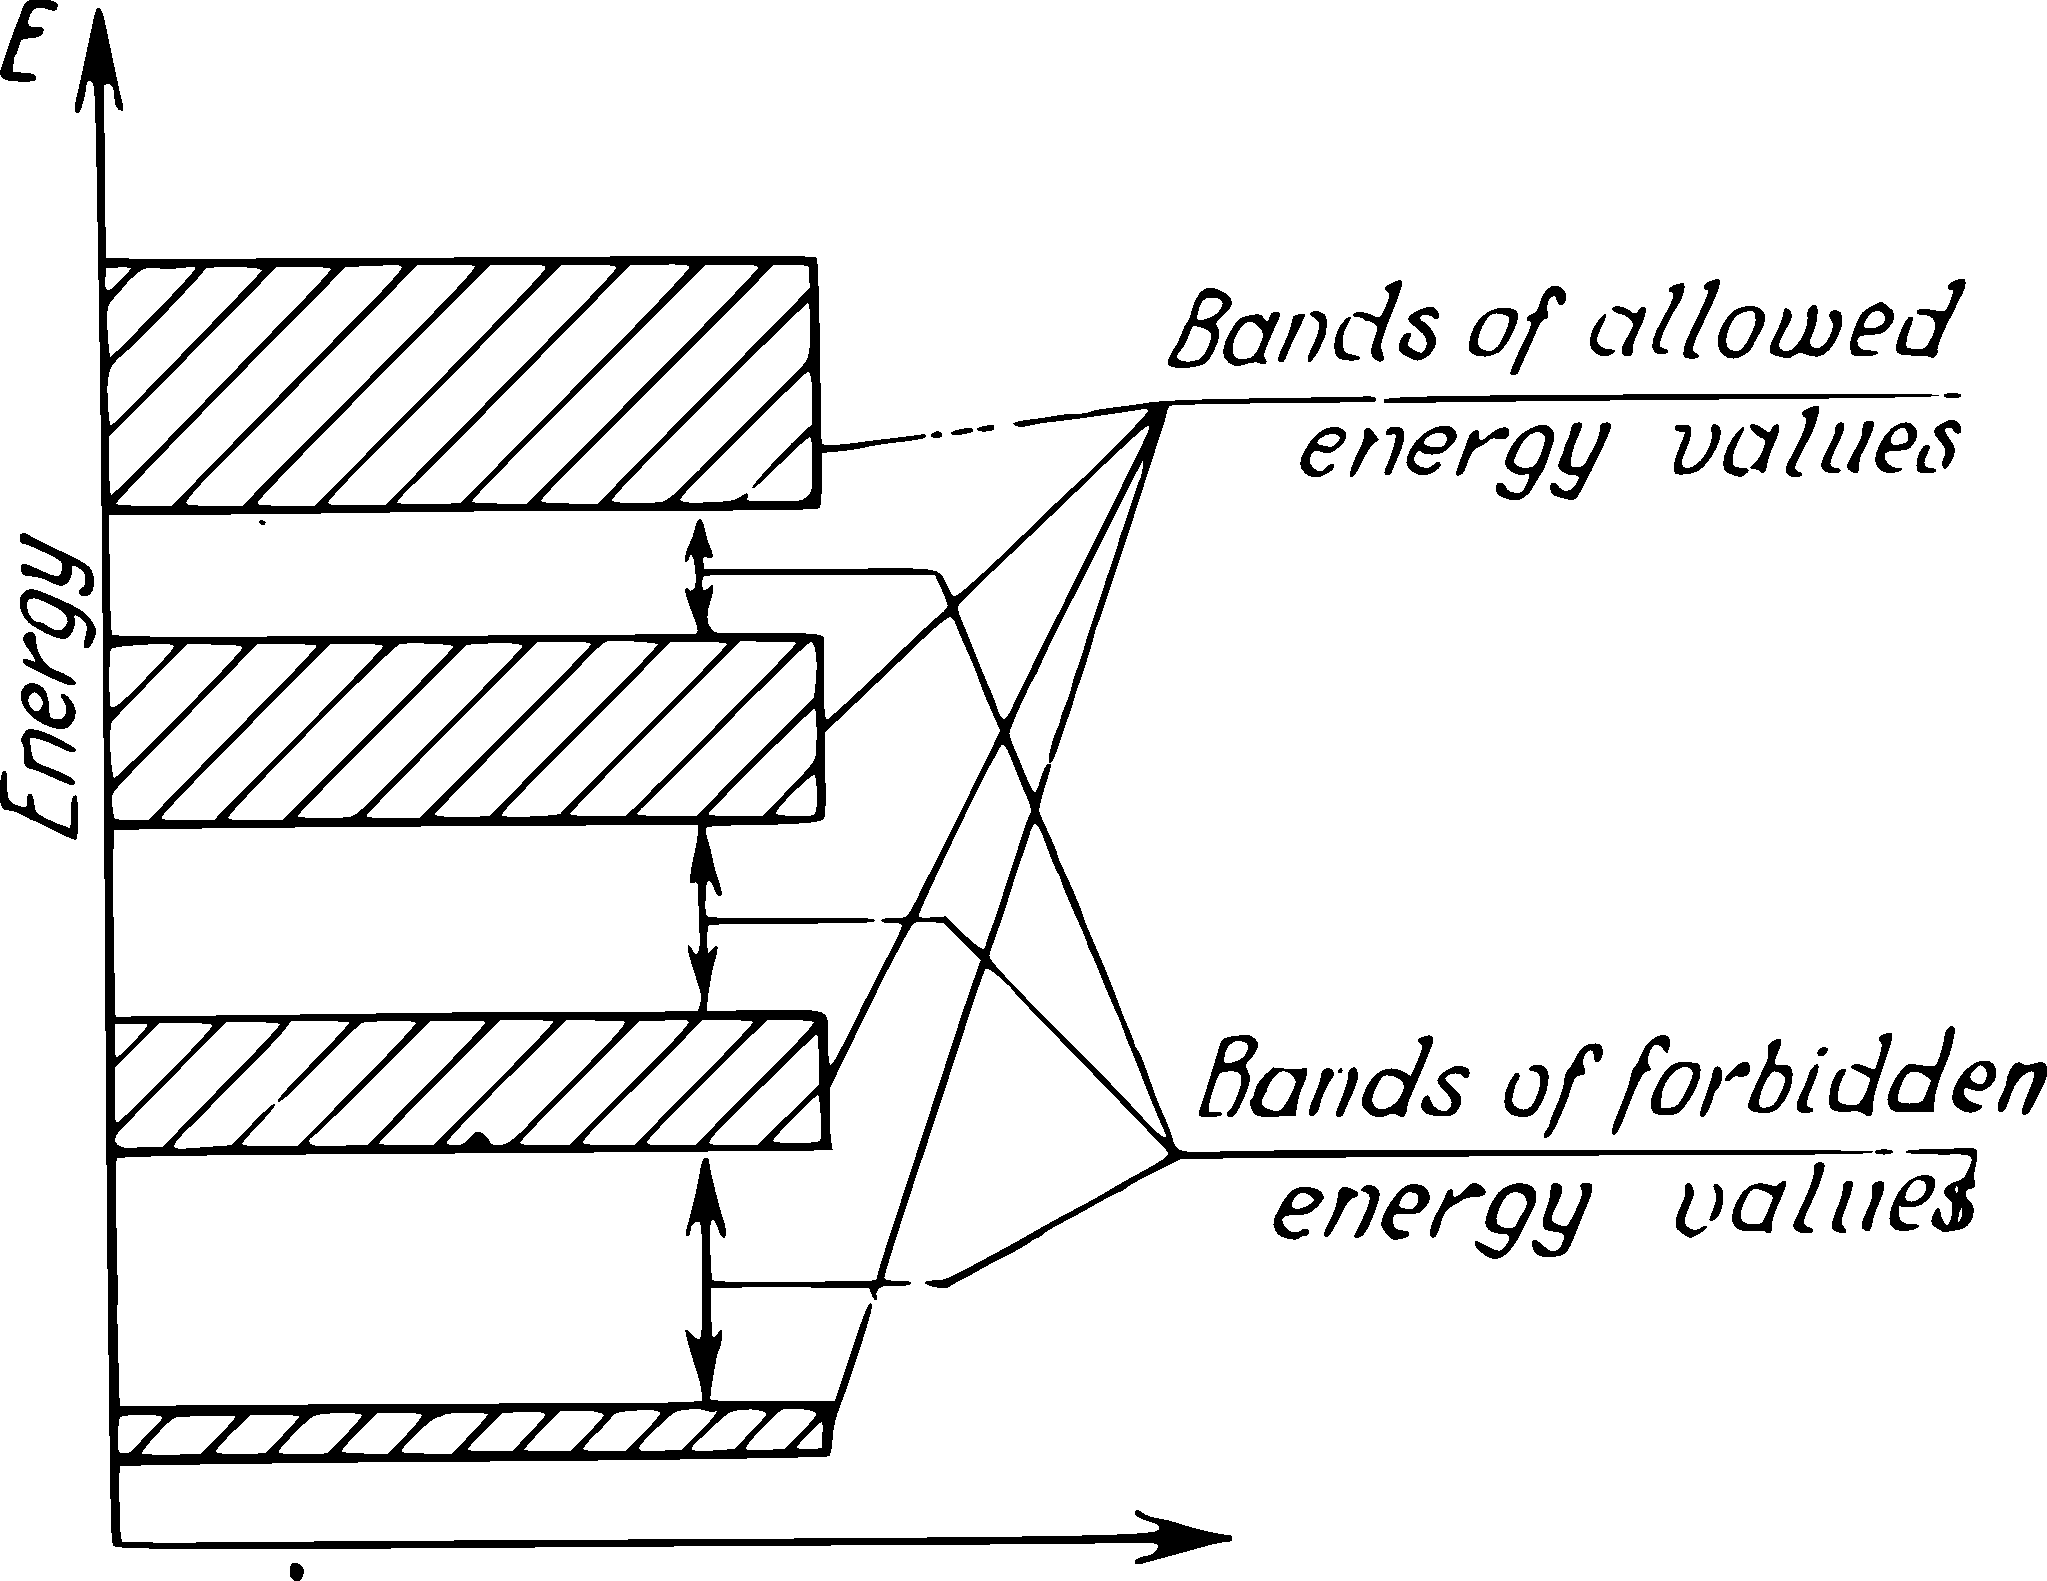
\includegraphics[width=0.8\textwidth]{figs/ch-41/fig-41-12.pdf}
\sidecaption{A schematic diagram of the energy bands of a solid.\zhcap{固体能带的示意图。}\label{fig-41-12}}
\end{figure}

\subsection{}\label{41.8.6} The allowed energy bands in a solid can be filled in different ways by electrons. In limiting cases they can be completely \ssect{41.9.1}. The electrons in a solid can move from one allowed band to another. For an electron to move from a lower band to the next higher one it is necessary to expend energy equal to the width of the forbidden band between the two allowed ones (of the order of several eV).
\zhpar{固体中的允许能带可以以各种不同方式被电子填充，在极限情形下它们可以被完全充满（参见\ssect{41.9.1}）。固体中的电子可以从一个允许能带转移到另一个允许能带。若要使电子从较低能带跃迁到相邻的较高能带，所需消耗的能量等于两个允许能带之间的禁带宽度（约为数个 eV 的量级）。}

Very little energy is required for intraband transitions. For
example, an energy of \num{d-4} to $\SI{d-8}{\electronvolt}$ is sufficient for this purpose, and it is acquired by an electron in a metal by the action of an electric field over a free path length at ordinary potential differences. But this energy is insufficient to move an  electron from one band to another. The action of thermal excitation can impart various energies to electrons, sufficient both for intraband and interband transitions.
\zhpar{能带内的跃迁所需的能量很小。例如，只需要 \num{d-4} 至 $\SI{d-8}{\electronvolt}$ 的能量即可实现这种跃迁，在普通电势差下，金属中的电子在一个自由程内受电场作用即可获得这一能量。但这一能量不足以使电子从一个能带跃迁到另一个能带。热激发可以使电子获得各种不同的能量，既足以引起能带内的跃迁，也足以引起能带间的跃迁。}


\section{Metals and Dielectrics in the Band Theory}
\label{sec-41.9} 
\zhtitle{能带理论中的金属与电介质}


\subsection{}\label{41.9.1} Differences in the electric properties of solids are explained by the band theory \ssect{41.8.2} by the fact that the allowed energy bands \ssect{41.8.2} are differently filled by electrons and by
the different widths of the forbidden bands \ssect{41.8.5}. These two factors determine whether a given solid is a conductor of electric current or is a dielectric. A necessary condition for a solid to be a conductor is the availability of empty energy levels to which the electric field can raise the electrons. It should be taken into consideration that the field can bring about only intraband transitionsjof the electrons \ssect{41.8.6}.

\zhpar{固体电学性质的差异可以由能带理论加以解释：其原因在于允许能带被电子填充的情况不同，以及禁带宽度不同（\ssect{41.8.2}，\ssect{41.8.5}）。这两个因素决定了某一固体是导电体还是电介质。固体成为导体的必要条件是存在空的能级，电场可以将电子提升到这些能级上。应当注意，电场只能引起电子的能带内跃迁（\ssect{41.8.6}）。}
\subsection{}\label{41.9.2} Typical examples of conductors are the metals of the first group of Mendeleev's periodic table \ssect{39.3.5}, for instance, sodium. In a single atom of sodium there are two filled electron shells, containing 2 and 8 electrons, respectively \ssect{39.3.4}.
\zhpar{导体的典型例子是门捷列夫周期表中第一族的金属，例如钠（\ssect{39.3.5}）。单个钠原子中有两个充满的电子壳层，分别含 2 个和 8 个电子（\ssect{39.3.4}）。}

According to the Pauli principle \ssect{39.3.1}, the eleventh valence electron of the sodium atom only fills half of the upper energy level. In a crystal of sodium, the first two filled shells of single atoms correspond to the energy bands completely filled with electrons.
\zhpar{根据泡利原理（\ssect{39.3.1}），钠原子的第十一个价电子只能填充其最高能级的一半。在钠晶体中，单个原子的前两个充满的壳层对应于被电子完全填满的能带。}

\begin{marginfigure}%[1cm] 
\centering
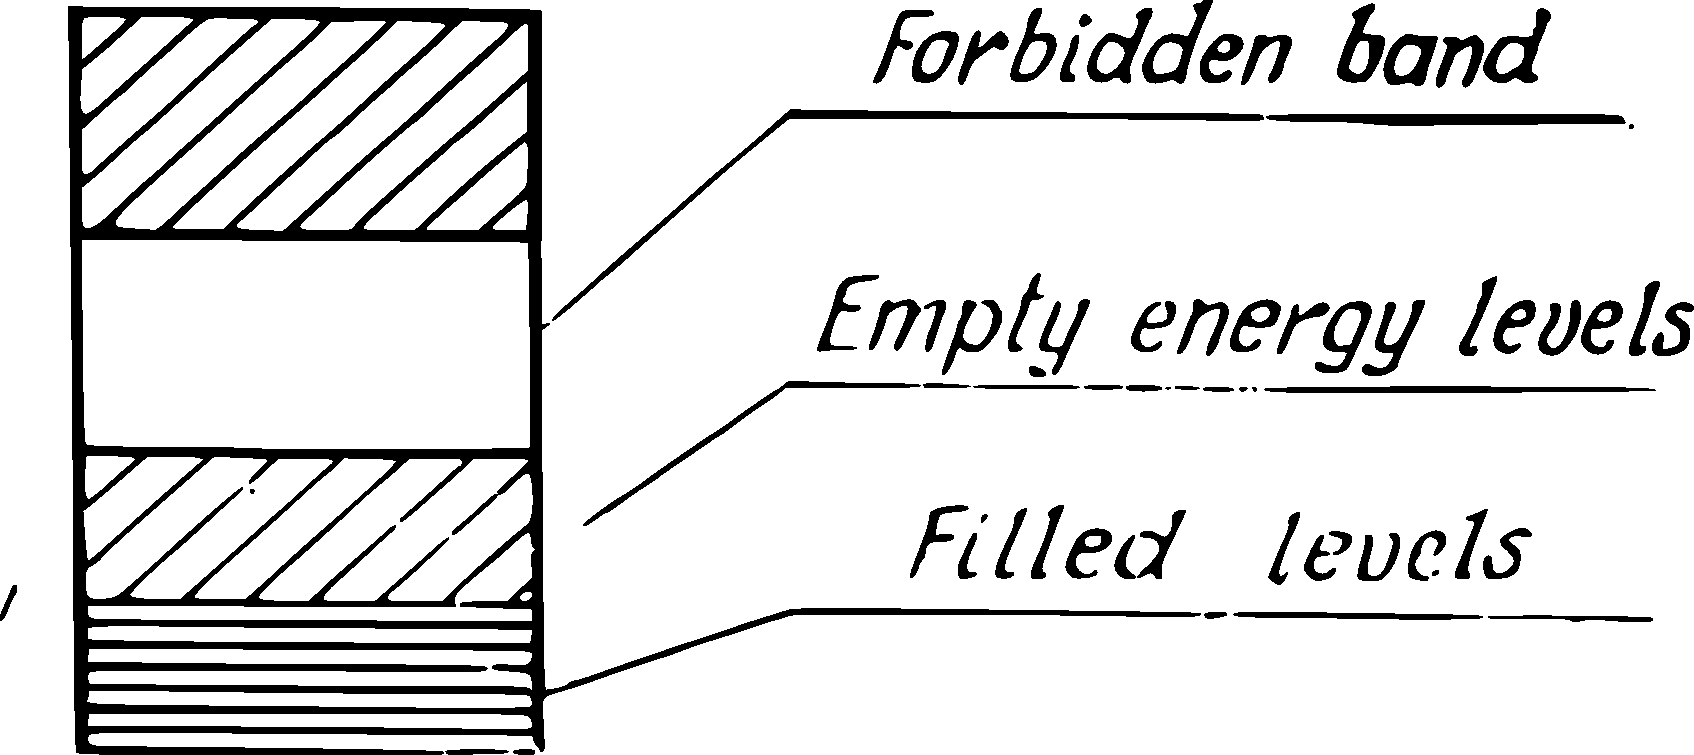
\includegraphics[width=\textwidth]{figs/ch-41/fig-41-13.pdf}
\sidecaption{Schematic representation of forbidden and empty energy levels of electron in a solid.\zhcap{固体中电子的禁带与空能级示意图。}\label{fig-41-13}}
\end{marginfigure}

The valence electrons of the sodium atoms in a crystal half
fill the levels of the band of allowed energy values (horizontally hatched in \figr{fig-41-13}). This is called the \redem{conduction band} because the electrons in it participate in producing the conduction current \ssect{20.1.2}. By the action of the electric field, set up in the crystal by the source of electrical energy, the valence electrons acquire more energy and move to higher, unoccupied energy levels in the conduction hand. This initiates their ordered motion and produces a current in the crystal.
\zhpar{钠晶体中的价电子半填充了允许能量值所对应的能带（图中水平阴影部分，见\figr{fig-41-13}）。这一能带称为\redem{导带}，因为其中的电子参与形成传导电流（\ssect{20.1.2}）。在晶体中电源所建立的电场作用下，价电子获得更多能量，并跃迁到导带中更高的未被占据的能级上。这引起了电子的定向运动，从而在晶体中产生电流。}

Thus, if the band is not completely occupied by valence electrons, a solid is always a conductor of electric current.
\zhpar{因此，若能带未被价电子完全占据，则固体总是导电体。}

\subsection{}\label{41.9.3} 

\redem{Hybridization} of allowed energy bands may occur in crystals. A band formed in splitting an upper excited level may overlap a band produced by the splitting of a lower state of valence electrons. This phenomenon is observed in the crystals of elements of the second group in Mendeleev's periodic table (\ce{Be}, \ce{Cd}, \ce{Mg}, \ce{Zn} and others). This forms a wider \redem{hybrid band} in which valence electrons are located, filling it only partly. Hence, a hybrid band is a conduction band, and such crystals are conductors of electric current.
\zhpar{晶体中允许能带可能发生\redem{杂化}。由上方激发能级分裂形成的能带，可能与由价电子较低态分裂产生的能带发生重叠。门捷列夫周期表中第二族元素（\ce{Be}、\ce{Cd}、\ce{Mg}、\ce{Zn} 等）的晶体中即观察到这一现象。这样便形成了一个更宽的\redem{杂化能带}，价电子位于其中，且只部分填充该能带。因此，杂化能带是导带，这类晶体是导电体。}

\subsection{}\label{41.9.4}

The energy bands do not overlap in solid dielectrics, and the band that combines the energy levels of the valence electrons of atoms or ions is completely filled with electrons, whereas all higher bands are entirely empty at $T = \SI{0}{\kelvin}$. The band completely filled with electrons is called the \redem{valence band}. The empty bands are conduction bands. An example of a crystalline dielectric is common salt (\ce{NaCl}). The NaCl molecule has a heteropolar bond \ssect{39.4.4}, which leads to the formation of \ce{Na+} and \ce{Cl-} ions with completely filled electron shells. The \ce{NaCl} crystal has a valence band of the \ce{Cl-} ion and all lower bands are completely filled, whereas the upper \ce{Na+} ion band, located above, is entirely empty. The \ce{Cl-} and \ce{Na+} bands are separated by \SI{6}{\electronvolt}, and the source of electrical energy cannot excite the electrons from the completely filled \ce{Cl-} band to the empty \ce{Na+} conduction band. This explains the dielectric properties of \ce{NaCl}.
\zhpar{在固体电介质中，能带之间不发生重叠。结合原子或离子价电子能级的能带被电子完全填满，而所有更高的能带在 $T = \SI{0}{\kelvin}$ 时都完全空着。被电子完全填满的能带称为\redem{价带}，空的能带则是导带。食盐（\ce{NaCl}）是晶体电介质的一个例子。\ce{NaCl} 分子具有异极键（\ssect{39.4.4}），由此形成了电子壳层充满的 \ce{Na+} 离子与 \ce{Cl-} 离子。\ce{NaCl} 晶体中，\ce{Cl-} 离子的能带为价带，所有更低的能带都被完全填满，而位于其上方的 \ce{Na+} 离子能带则完全空着。\ce{Cl-} 能带与 \ce{Na+} 能带之间相隔 \SI{6}{\electronvolt}，电源无法将电子从被完全填满的 \ce{Cl-} 能带激发到空的 \ce{Na+} 导带中。这就解释了 \ce{NaCl} 的电介质性质。}

\clearpage

\section{Electrical Conduction of Semiconductors}
\label{sec-41.10} 
\zhtitle{半导体的导电}


\subsection{}\label{41.10.1} \redem{Semiconductors} include a large class of substances whose resistivity varies in a wide range from \num{d-6} to \SI{d8}{\ohm\metre}, and is reduced very rapidly, according to an exponential law, as the temperature is raised \ssect{41.10.2}. The most typical and extensively employed semiconductor materials are the chemical elements germanium, silicon, and tellurium. In the outer shell of germanium and silicon atoms there are four valence electrons, which form covalent bonds \ssect{39.4.5} with the valence electrons of adjacent atoms. There are no ``free'' valence electrons in chemically pure crystals of these semiconductors. On the basis of the band theory \ssect{41.8.2} crystalline semiconductors belong to the type of solids in which the valence band \ssect{41.9.4} is separated from the empty conduction band (at \(T = \SI{0}{\kelvin}\)) by a comparatively narrow energy region \(\Delta E_0 \) (\figr{fig-41-14}), less than that in dielectric crystals \ssect{41.9.4}.
\zhpar{\redem{半导体}是一大类物质，其电阻率变化范围很大，从 \num{d-6} 到 \SI{d8}{\ohm\metre}，并且随温度升高按指数规律迅速减小（\ssect{41.10.2}）。最典型、应用最广泛的半导体材料是锗、硅和碲等化学元素。锗和硅原子的最外层壳层有四个价电子，它们与相邻原子的价电子形成共价键（\ssect{39.4.5}）。在化学纯的这些半导体晶体中，不存在“自由”的价电子。根据能带理论（\ssect{41.8.2}），晶体半导体属于这样一类固体：其价带（\ssect{41.9.4}）与 $T = \SI{0}{\kelvin}$ 时空的导带之间，被一个相对较窄的能量区域 \(\Delta E_0 \)（见\figr{fig-41-14}）隔开，该区域宽度小于电介质晶体中的相应宽度（\ssect{41.9.4}）。}

\begin{marginfigure}%[-3cm] 
\centering
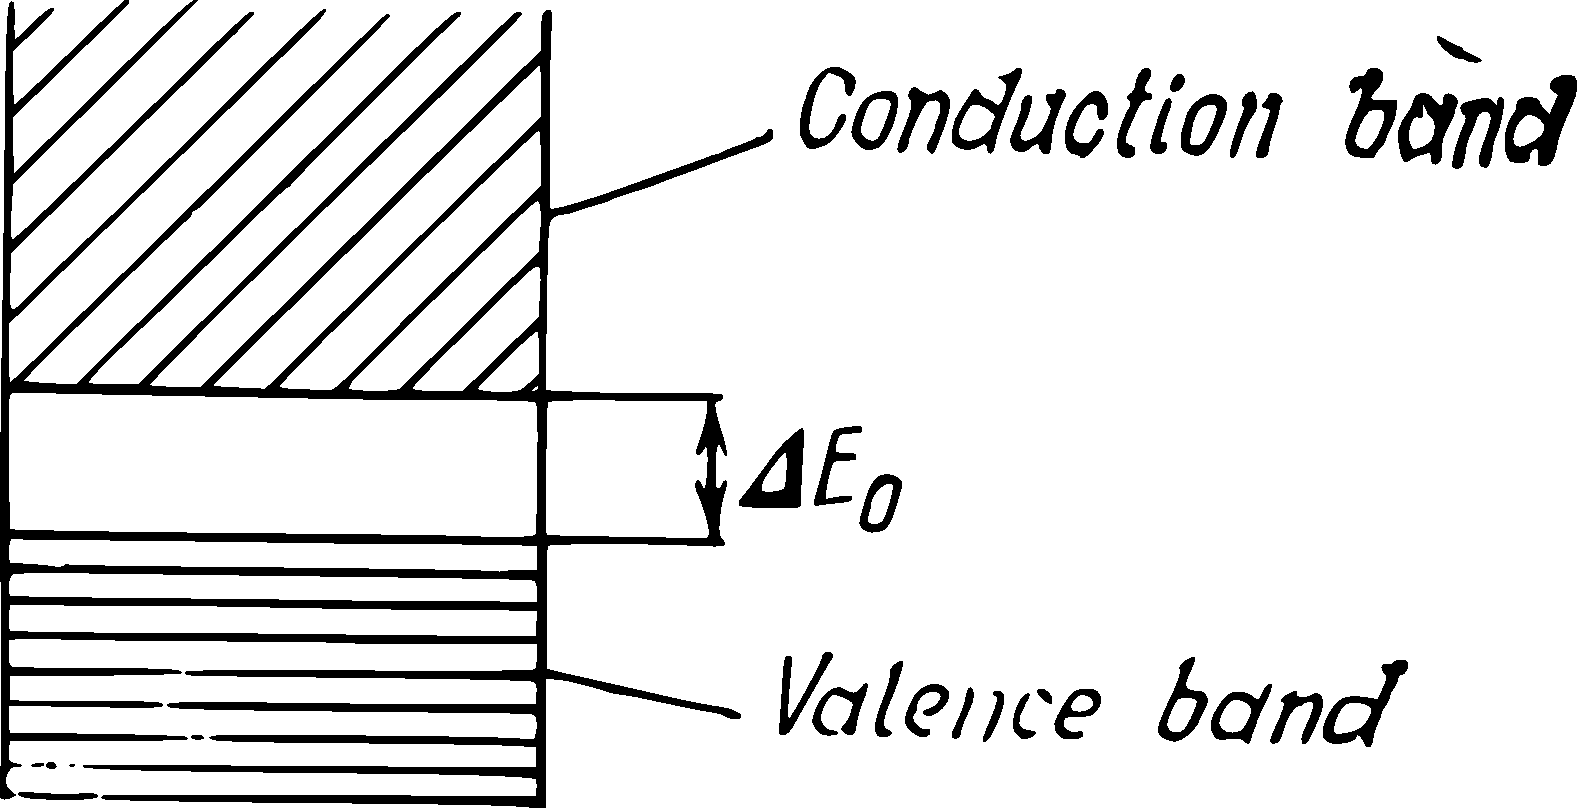
\includegraphics[width=\textwidth]{figs/ch-41/fig-41-14.pdf}
\sidecaption{The separation of conduction and valence bands in semiconductors.\zhcap{半导体中导带与价带的分隔。}\label{fig-41-14}}
\end{marginfigure}


For silicon \(\Delta E_0 = \SI{1.1}{\electronvolt}\);  
for germanium \(\Delta E_0 = \SI{0.72}{\electronvolt}\).
\zhpar{对于硅，\(\Delta E_0 = \SI{1.1}{\electronvolt}\)；对于锗，\(\Delta E_0 = \SI{0.72}{\electronvolt}\)。}

\subsection{}\label{41.10.2}

Conduction of chemically pure semiconductors is called the \redem{intrinsic conduction}. \redem{Electron conduction ($n$-type conduction)} occurs when electrons are transferred from the valence band to the conduction band. This requires an expenditure of energy, not less than the width \(\Delta E_0\) of the forbidden band (\figr{fig-41-14}). The quantity \(\Delta E_0\) is called the \redem{activation energy} of intrinsic conduction. As the temperature of the semiconductor is raised, an increased number of electrons move from the valence band to the conduction band and participate in electrical conduction. The conductivity \ssect{20.3.4} of semiconductors increases with the temperature \(T\) according to the law
\zhpar{化学纯半导体的导电称为\redem{本征导电}。电子从价带转移到导带时发生的导电，称为\redem{电子导电}（\redem{$n$ 型导电}）。这需要消耗能量，所需能量不小于禁带宽度 $\Delta E_0$（见\figr{fig-41-14}）。量 $\Delta E_0$ 称为本征导电的\redem{激活能}。随着半导体温度升高，越来越多的电子从价带跃迁到导带并参与导电。半导体的电导率（\ssect{20.3.4}）随温度 $T$ 按下列规律增大：}
\begin{equation*}%
\varkappa = \varkappa_{0} \exp \left(-\frac{\Delta E_{0}}{2kT} \right), 
\end{equation*}
where \(k\) is Boltzmann's constant \ssect{8.4.5}. The resistivity \ssect{20.3.4} of semiconductors drastically decreases as the temperature is raised according to the relation
\zhpar{式中 \(k\) 为玻尔兹曼常量（\ssect{8.4.5}）。半导体的电阻率（\ssect{20.3.4}）随温度升高按下列关系急剧减小：}
\begin{equation*}%
\rho = \rho_{0} \exp \left(\frac{\Delta E_{0}}{2kT} \right)
\end{equation*}
This feature of semiconductors essentially differentiates them from metals \ssect{20.3.7}.
\zhpar{半导体的这一特性与金属有本质区别（\ssect{20.3.7}）。}

\subsection{}\label{41.10.3}

The transition of an electron from the valence band of a semiconductor to the conduction band indicates that the covalent bonds \ssect{39.4.5} of the atoms are violated in the semiconductor crystal. A certain one of the valence electrons of one of the atoms in the lattice leaves its place. The abandoned place, or vacancy, displays surplus positive charge. Such a vacancy is called a \redem{positive hole}, and is treated as a positive charge carrier. In the band theory this means that a vacant energy level appears in the valence band of the crystal.
\zhpar{电子从半导体价带跃迁到导带，表明半导体晶体中原子之间的共价键遭到破坏。晶格中某个原子的某个价电子离开了原来的位置。被遗弃的位置，即空位，显示出多余的正电荷。这种空位称为\redem{正空穴}，并被视为正电荷载流子。在能带理论中，这意味着晶体的价带中出现了一个空的能级。}

A positive hole behaves like a positive charge, equal in magnitude to the charge of the electron. Another electron may move to the place (hole) abandoned by the previous electron. This is equivalent to the movement of the positive hole; it appears at a new place, left by the second electron. In the external electric field, the electrons throughout the mass of the semiconductor move in the direction opposite to that of the electric field strength \ssect{15.1.2}. The positive holes move in the direction of the field strength, i.e. in the direction that a positive charge would travel when subject to an electric field. 
\zhpar{正空穴的行为与正电荷相同，其电荷量与电子电荷的大小相等。另一个电子可能移动到前一个电子所遗弃的位置（空穴）上。这等效于正空穴的移动：它出现在第二个电子所留下的新位置上。在外电场中，半导体体内的电子沿与电场强度相反的方向运动（\ssect{15.1.2}），而正空穴则沿电场强度方向运动，即沿正电荷在电场中运动的方向运动。}

The electrical conduction of a semiconductor that is due to the motion of holes is called \redem{hole}, or \redem{$p$-type, conduction}.
\zhpar{半导体中由空穴运动引起的导电称为\redem{空穴导电}，或\redem{$p$ 型导电}。}

\subsection{}\label{41.10.4} The intrinsic conduction of semiconductors is due to the presence of two kinds of current carriers: electrons in the conduction band and holes in the valence band. Each electron excited to the conduction band corresponds to one hole in the valence band. The electron concentration $n_{e}$ and hole concentration $n_{h}$ are the same and increase rapidly with the temperature $T$ according to the law
\zhpar{半导体的本征导电源于两种载流子的存在：导带中的电子和价带中的空穴。每一个被激发到导带中的电子，都对应于价带中的一个空穴。电子浓度 $n_{e}$ 与空穴浓度 $n_{h}$ 相等，并且随温度 $T$ 按下列规律迅速增大：}
\begin{equation*}%
n_{e} = n_{h} = \text{const } \exp \left(-\frac{\Delta E_{0}}{2kT} \right),
\end{equation*}
where $\Delta E_{0}$ is the activation energy of intrinsic conduction \ssect{41.10.2} , and $k$ is Boltzmann's constant \ssect{8.4.5}. This explains the nature of the dependence of the electrical conductivity and resistivity of semiconductors \ssect{41.10.2} on the temperature, which strongly differs from the dependence of these quantities in metals \ssect{20.3.7}.
\zhpar{式中 $\Delta E_{0}$ 为本征导电的激活能（\ssect{41.10.2}），$k$ 为玻尔兹曼常量（\ssect{8.4.5}）。由此可以解释半导体的电导率和电阻率随温度变化的性质（\ssect{41.10.2}），这种变化关系与金属中的情形有很大不同（\ssect{20.3.7}）。}

\subsection{}\label{41.10.5} The electrical conduction of semiconductors due to the presence in them of impurity centres is called \redem{extrinsic}, or \redem{impurity, conduction}.
\zhpar{半导体中因存在杂质中心而引起的导电，称为\redem{非本征导电}，或\redem{杂质导电}。}

\redem{Impurity centres} (or simply \redem{impurities}) may be atoms or ions of foreign elements, and various defects and distortion of the crystal lattice (vacant points, displacements due to deformation of the crystal, etc.).
\zhpar{\redem{杂质中心}（或简称\redem{杂质}）可以是外来元素的原子或离子，也可以是各种缺陷和晶格畸变（如空位、由晶体形变引起的位移等）。}

Impurities change the periodic electric field in a solid and affect the motion of the electrons and their energy states. The energy levels of the valence electrons of impurity atoms are not located in the allowed energy bands \ssect{41.9.2} of the main, or host, crystal, and \redem{impurity energy levels} (\redem{localized levels}) are formed in the forbidden band.
\zhpar{杂质会改变固体中的周期性电场，并影响电子的运动及其能态。杂质原子价电子的能级不位于主晶体（基质晶体）的允许能带（\ssect{41.9.2}）之内，而是在禁带中形成\redem{杂质能级}（\redem{局域能级}）。}
\begin{marginfigure}%[-3cm] 
\centering
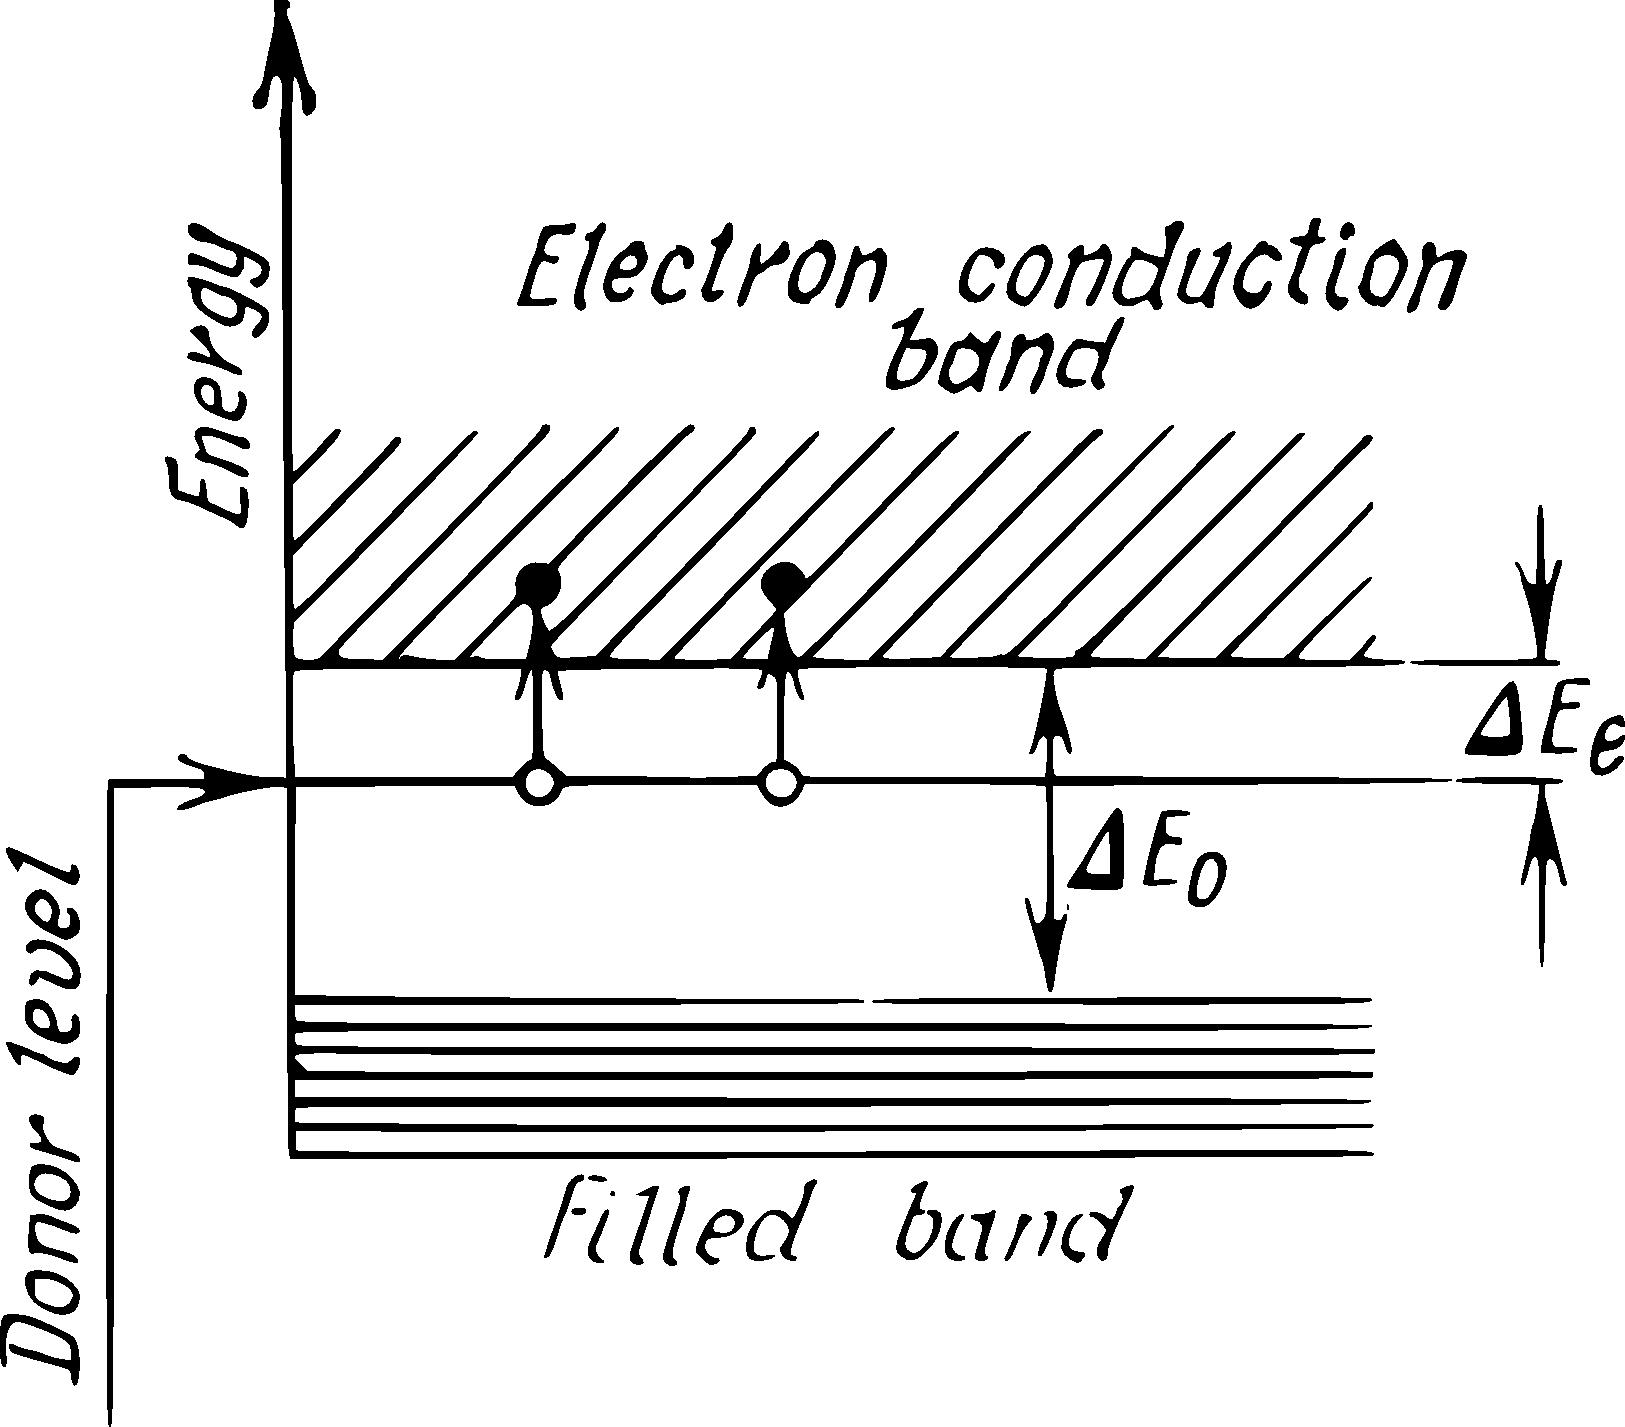
\includegraphics[width=\textwidth]{figs/ch-41/fig-41-15.pdf}
\sidecaption{Effect of pentavalent impurity on electron energy levels in bands.\zhcap{五价杂质对能带中电子能级的影响。}\label{fig-41-15}}
\end{marginfigure}

\subsection{}\label{41.10.6} Impurities can be a supplementary source of electrons in a solid. For example, in the substitution of one tetravalent atom of germanium by an atom of an impurity having five valence electrons (phosphorus, antimony or arsenic) one of the electrons of the impurity cannot form a covalent bond \redem{39.4.5} with the germanium atoms and is thereby ``superfluous''. The energy levels of such electrons are below the conduction band of the host crystal (\figr{fig-41-15}). Such levels, filled with electrons, are called \redem{donor levels}, and the atoms of the impurity that supply the ``superfluous'' electrons are called \redem{donor atoms}. 
\zhpar{杂质可以成为固体中电子的额外来源。例如，用一个具有五个价电子的杂质原子（磷、锑或砷）替代锗晶体中的一个四价锗原子时，杂质的一个电子无法与锗原子形成共价键（\ssect{39.4.5}），因而成为“多余”的电子。这些电子的能级位于主晶体导带之下（见\figr{fig-41-15}）。这类被电子占据的能级称为\redem{施主能级}，提供“多余”电子的杂质原子称为\redem{施主原子}。}




Only a small amount of energy $\Delta E_{e}$ is required to excite electrons from the donor levels to the conduction band. This energy is obtained, for instance, from thermal excitation. For silicon $\Delta E_{e} = \SI{0.054}{\electronvolt}$ if the impurity is arsenic. When electrons are transferred from the donor levels to the conduction band, \redem{electron impurity}, or \redem{extrinsic, conduction ($n$-type impurity conduction)} occurs. Such semiconductors are called \redem{electron impurity semiconductors (n-type semiconductors)}.
\zhpar{使电子从施主能级激发到导带所需的能量 $\Delta E_{e}$ 很小，例如可由热激发提供。若杂质为砷，则对于硅，$\Delta E_{e} = \SI{0.054}{\electronvolt}$。当电子从施主能级转移到导带时，发生\redem{电子杂质导电}，或称\redem{非本征导电}（\redem{$n$ 型杂质导电}）。这类半导体称为\redem{电子型杂质半导体}（\redem{$n$ 型半导体}）。}

\subsection{}\label{41.10.7} If a tetravalent atom in the lattice of the semiconductor is replaced by a trivalent impurity atom (boron, aluminium or indium) there will be a lack of one electron to form saturated covalent bonds. The lacking electron can be borrowed from the lattice of the neighbouring atom of germanium, in which a positive hole is thereby formed \ssect{41.10.3}. The consecutive filling
of the holes formed in the germanium atoms by electrons is
equivalent to the movement of the holes and leads to conduction in the semiconductor. The impurity energy levels, not occupied by electrons, are called \redem{trapping}, or \redem{acceptor, levels}. In this case, the impurity atoms are said to he acceptor atoms. 
\zhpar{若半导体晶格中的四价原子被三价杂质原子（硼、铝或铟）替代，则缺少一个电子来形成饱和的共价键。缺少的电子可以从相邻锗原子的晶格中借来，这样就在该锗原子中形成了一个正空穴（\ssect{41.10.3}）。电子依次填充锗原子中形成的空穴，等效于空穴的移动，从而引起半导体中的导电。未被电子占据的杂质能级称为\redem{俘获能级}，或\redem{受主能级}。此时，杂质原子称为\redem{受主原子}。}

\begin{marginfigure}[-3cm] 
\centering
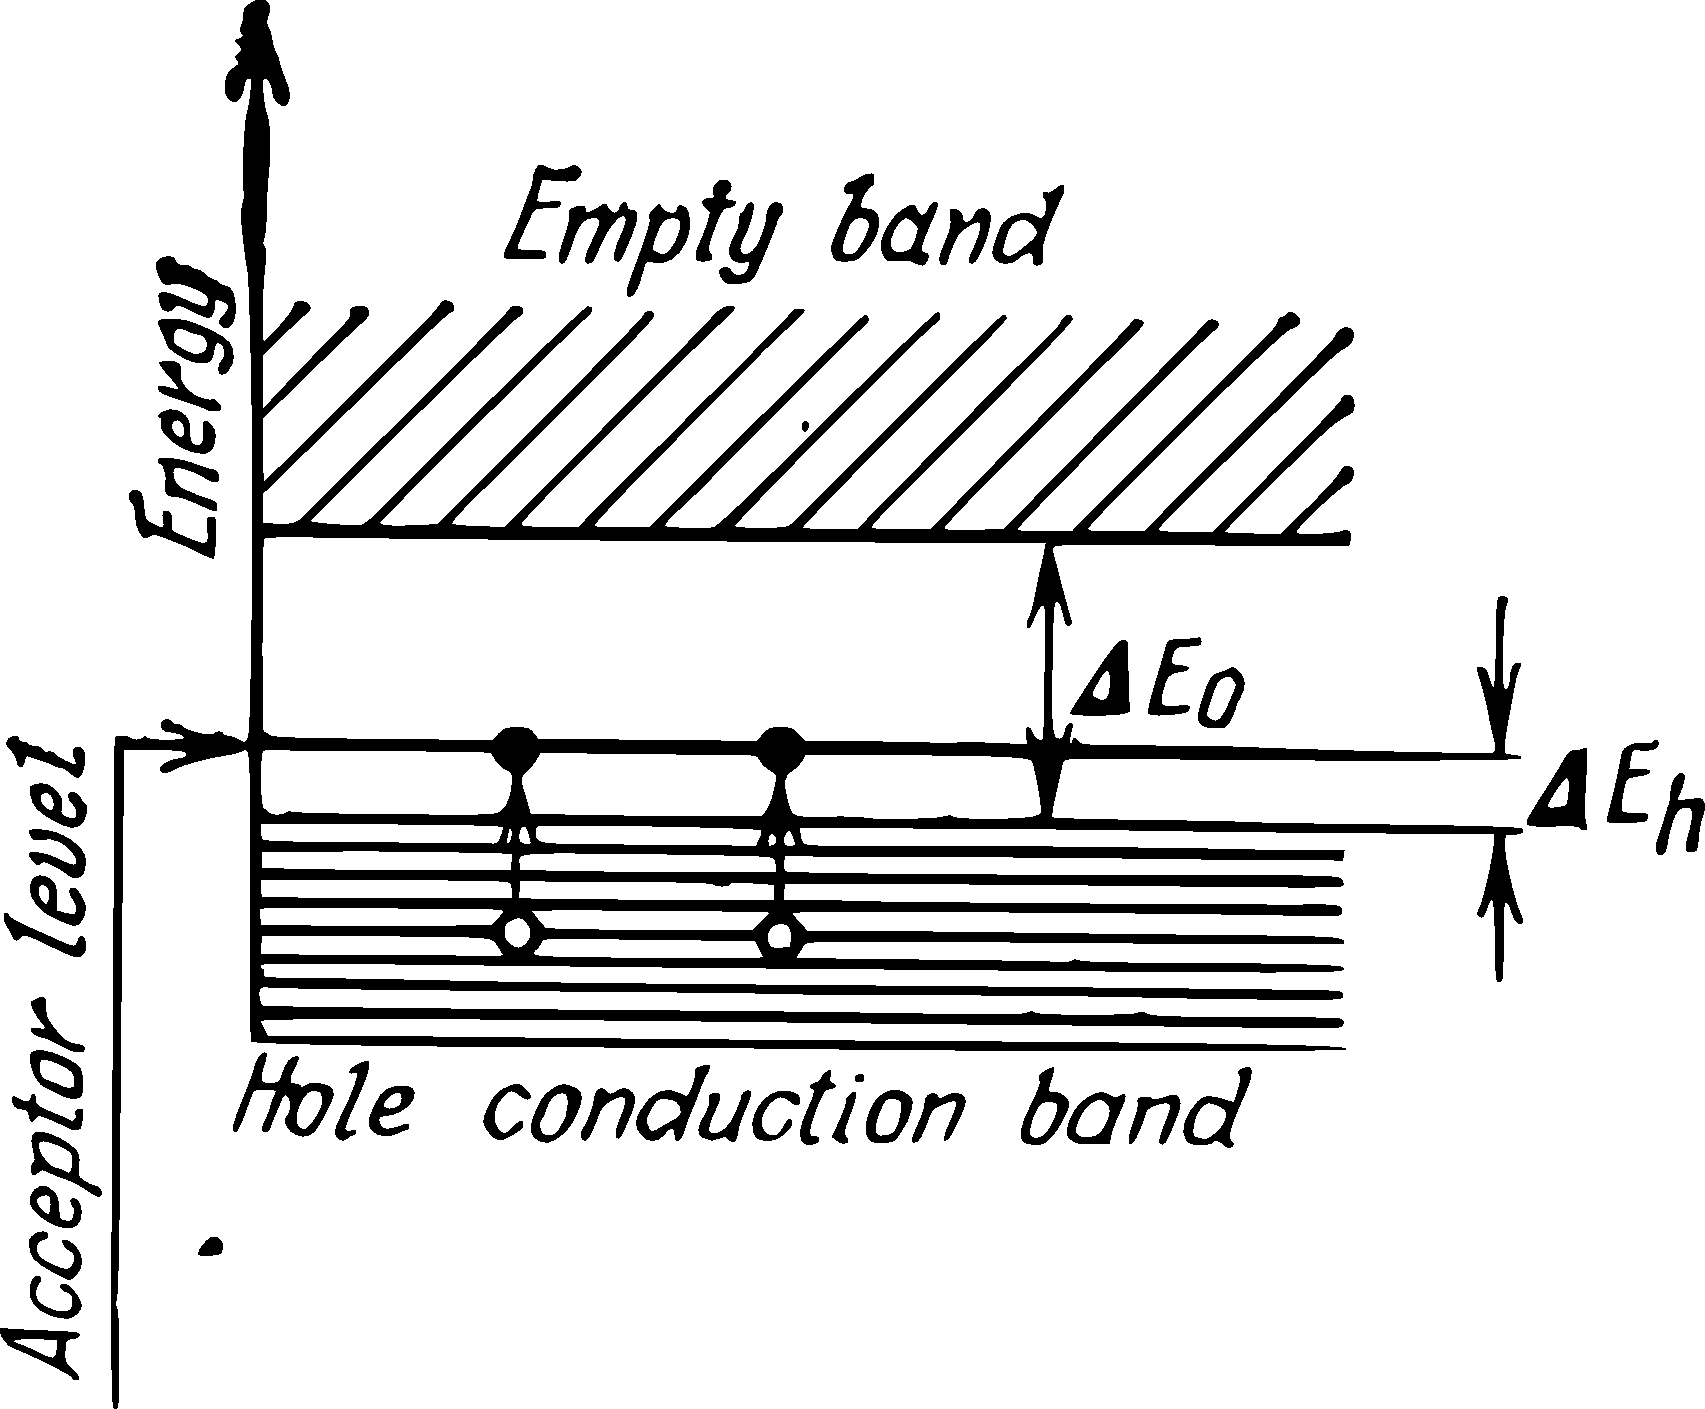
\includegraphics[width=\textwidth]{figs/ch-41/fig-41-16.pdf}
\sidecaption{Effect of triavalent impurity on electron energy levels in bands.\zhcap{三价杂质对能带中电子能级的影响。}\label{fig-41-16}}
\end{marginfigure}


Acceptor levels are located above the upper edge of the valence band \ssect{41.9.4} of the host crystal (\figr{fig-41-16}). When silicon crystals are doped with boron (the addition of impurities to a semicondductor is called doping), the acceptor levels are an amount $\Delta E_{h} = \SI{0.08}{\electronvolt}$ above the valence band. The transfer of electrons from the filled valence hand to the acceptor level produces positive holes in this band, and the valence band becomes a band of hole conduction. This leads to \redem{hole impurity conduction ($p$-type impurity conduction)}. Such semiconductors are called \redem{hole impurity semiconductors (p-type semiconductors)}.
\zhpar{受主能级位于主晶体价带（\ssect{41.9.4}）上边缘之上（见\figr{fig-41-16}）。当硅晶体中掺入硼时（向半导体中加入杂质称为掺杂），受主能级比价带高出 $\Delta E_{h} = \SI{0.08}{\electronvolt}$。电子从充满的价带转移到受主能级上，在价带中产生正空穴，价带变为空穴导电的能带。这就产生了\redem{空穴杂质导电}（\redem{$p$ 型杂质导电}）。这类半导体称为\redem{空穴型杂质半导体}（\redem{$p$ 型半导体}）。}

\subsection{}\label{41.10.8} When a semiconductor is doped with both donor and acceptor impurities at the same time, the nature of the conduction ($n$- or $p$-type) depends upon which impurity produces the higher concentration of current carriers. The concentration and energy of the electrons (and holes) in semiconductors depend very strongly, in contrast to those of metals, on the temperature, and increase when the temperature is raised.
\zhpar{当半导体同时掺入施主杂质和受主杂质时，导电类型（$n$ 型或 $p$ 型）取决于哪一种杂质产生的载流子浓度更高。与金属不同，半导体中电子（及空穴）的浓度和能量强烈依赖于温度，并随温度升高而增大。}

\section[Electrical Contact Phenomena]{Concept of Contact Electrical Phenomena in Metals and Semiconductors}
\label{sec-41.11} 
\zhtitle{金属与半导体中接触电现象的概念}

\begin{marginfigure}%[-3cm] 
\centering
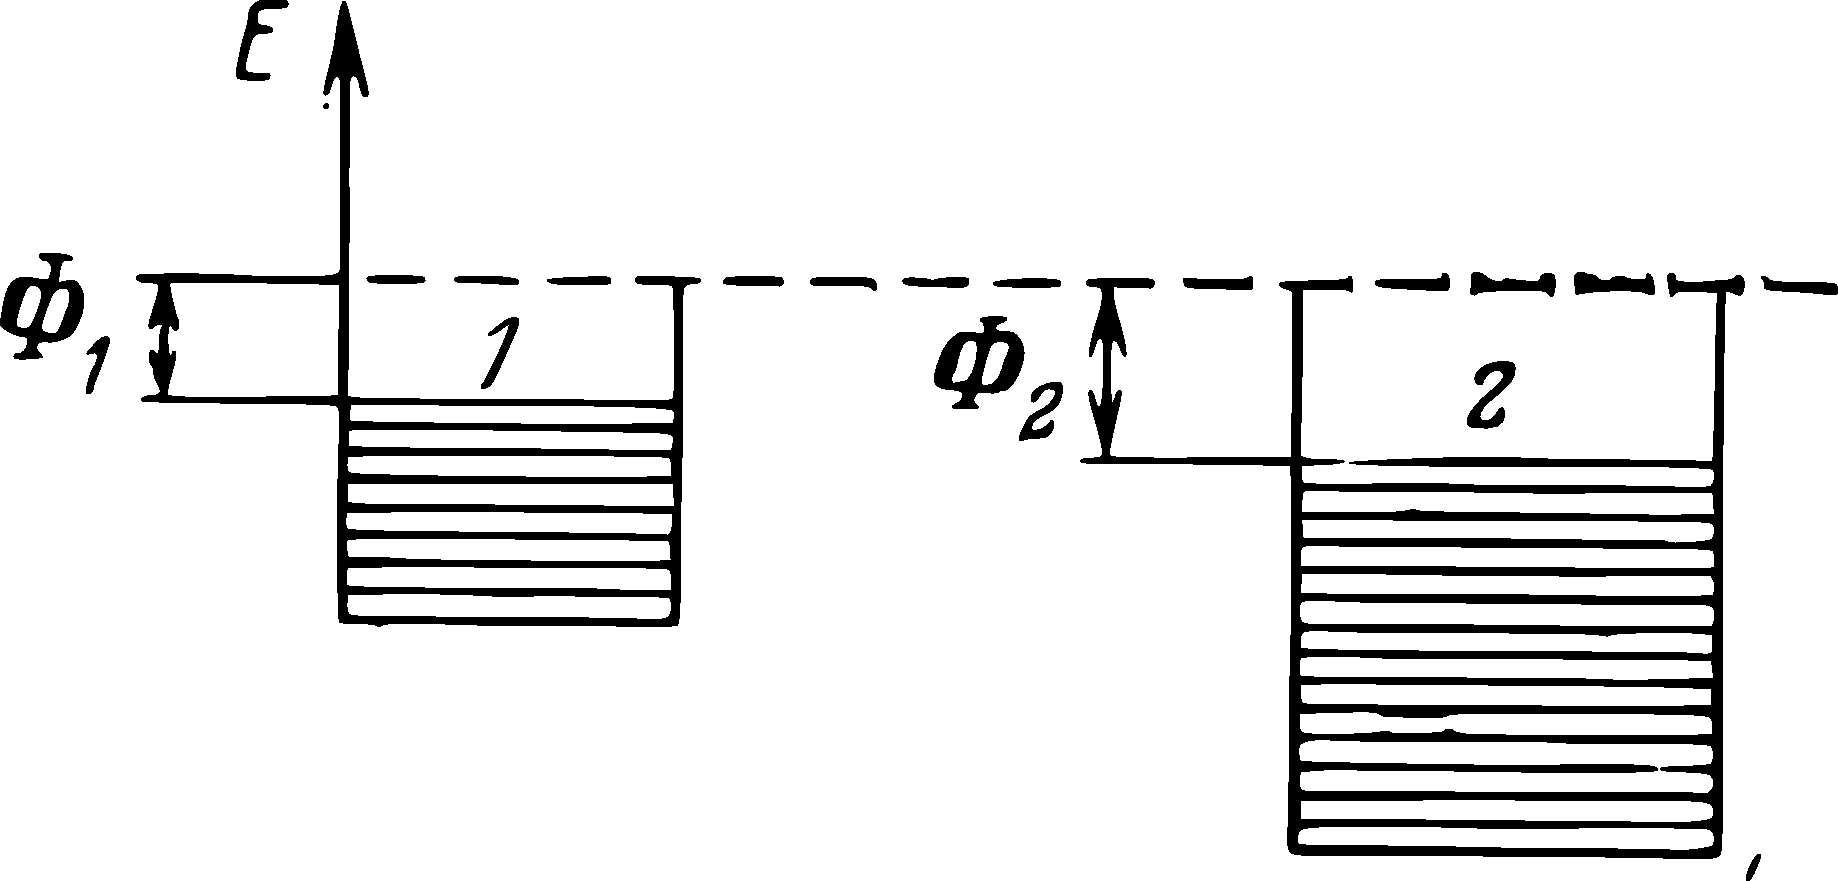
\includegraphics[width=\textwidth]{figs/ch-41/fig-41-17.pdf}
\sidecaption{The work function in metals.\zhcap{金属中的逸出功。}\label{fig-41-17}}
\end{marginfigure}


\subsection{}\label{41.11.1} The \redem{work function} $\Phi$ in removing an electron from a metal is the work it is necessary to do for the electron to emerge from the metal into vacuum. The work $\Phi$ is done against the attractive forces developed by the surplus positive charge in the metal resulting from the removal of the electron. Besides, it is necessary to overcome the repulsion forces of the previously emerged electrons if they have not been removed and form an
electron ``cloud'' at the surface of the conductor. The work
function has a value of the order of several eV and depends upon the kind of metal and the condition of its surface; it is changed by the presence of dirt, traces of moisture, etc. In the quantum theory of solids, the work function is reckoned from the upper electron-filled Fermi level \ssect{41.4.2} \figr{fig-41-17}).
\zhpar{从金属中移去一个电子所需的功，即电子从金属逸出到真空中所必须做的功，称为\redem{逸出功} $\Phi$。该功须克服金属中电子移出后留下的正电荷所产生的吸引力。此外，若先前逸出的电子没有被移去，并在导体表面形成电子“云”，则还须克服这些电子的斥力。逸出功的数量级为数个 eV，它取决于金属的种类及其表面状态，并会因表面存在污物、水汽痕迹等而改变。在固体的量子理论中，逸出功是从被电子占满的最高费米能级（\ssect{41.4.2}）算起的（见\figr{fig-41-17}）。}

\subsection{}\label{41.11.2} Since the fastest electrons fly out of the metal, a lack of negative charge is formed in the metallic conductor and a surplus in the surrounding space. This is evident in a very thin layer (of a thickness equal to several interatomic distances in the metal) on both sides of the surface of the conductor. It is contended that the surface of the metal is a \redem{double electric layer (contact layer) }similar to an extremely thin capacitor \ssect{17.2.4}.
\zhpar{由于速度最快的电子飞出金属，金属导体内部缺少负电荷，而周围空间则出现多余的负电荷。这种现象出现在导体表面两侧非常薄的一层中（其厚度约为金属中几个原子间距）。通常认为，金属表面是一个\redem{双电层}（\redem{接触层}），类似于一个极薄的电容器（\ssect{17.2.4}）。}

\subsection{}\label{41.11.3} The potential difference $\Delta V$ \ssect{16.2.7}, characterizing the electric field of the double layer, is called the \redem{surface potential jump} at the metal-vacuum boundary, or the \redem{contact potential difference} between a metal and a vacuum. Thus 
\zhpar{表征双电层电场的电势差 $\Delta V$（\ssect{16.2.7}），称为金属与真空边界处的\redem{表面电势跃变}，或金属与真空之间的\redem{接触电势差}。即：}
\begin{equation*}%
\Delta V = \frac{\Phi}{e},
\end{equation*}
where $\Phi$ is the work function \ssect{41.11.1}, and $e$ is the magnitude of the electron charge.
\zhpar{式中 $\Phi$ 为逸出功（\ssect{41.11.1}），$e$ 为电子电荷的大小。}

There is no electric field outside the double layer, and the potential outside the metal and beyond the double layer equals
zero. Inside the metal the potential is positive and equal to AF. The potential energy of the conduction electrons \ssect{20.3.1} is negative and is equal to $- e \Delta V = \Phi$. The whole volume of the metal is a potential well \ssect{38.4.1} for the conduction electrons; the depth of the well equals the work function $\Phi$.
\zhpar{双电层之外不存在电场，金属外部及双电层之外的电势为零。金属内部的电势为正，其值等于 $\Delta V$。导电电子的势能为负，且等于 $- e \Delta V = \Phi$。整个金属体积对于导电电子而言是一个势阱（\ssect{38.4.1}），势阱深度等于逸出功 $\Phi$。}

\subsection{}\label{41.11.4} In the contact of two dissimilar metals, $\mathit{1}$ and $\mathit{2}$, having the work functions $\Phi_{1}$ and $\Phi_{2}$ electrons pass predominantly from the metal with the lower work function to that with the higher one. The metals acquire unlike charges and, in a state of thermodynamic equilibrium \ssect{8.3.3}, there is a potential difference $\Delta V_{12}$ between the two contacting dissimilar metals. It is called the \redem{internal contact potential difference}.
\zhpar{两种不同金属 $\mathit{1}$ 与 $\mathit{2}$ 相接触，其逸出功分别为 $\Phi_{1}$ 和 $\Phi_{2}$，电子主要从逸出功较小的金属流向逸出功较大的金属。两金属分别带上异号电荷，并在热力学平衡状态（\ssect{8.3.3}）下，两相接触的异种金属之间存在电势差 $\Delta V_{12}$，称为\redem{内接触电势差}。}

The potential difference $\Delta V_{12}'$ between two points located close to but outside the surfaces of the first and second contacting metals is called the \redem{external contact potential difference}.
\zhpar{位于第一、第二两接触金属表面外侧附近的两点之间的电势差 $\Delta V_{12}'$，称为\redem{外接触电势差}。}

\begin{marginfigure}%[-3cm] 
\centering
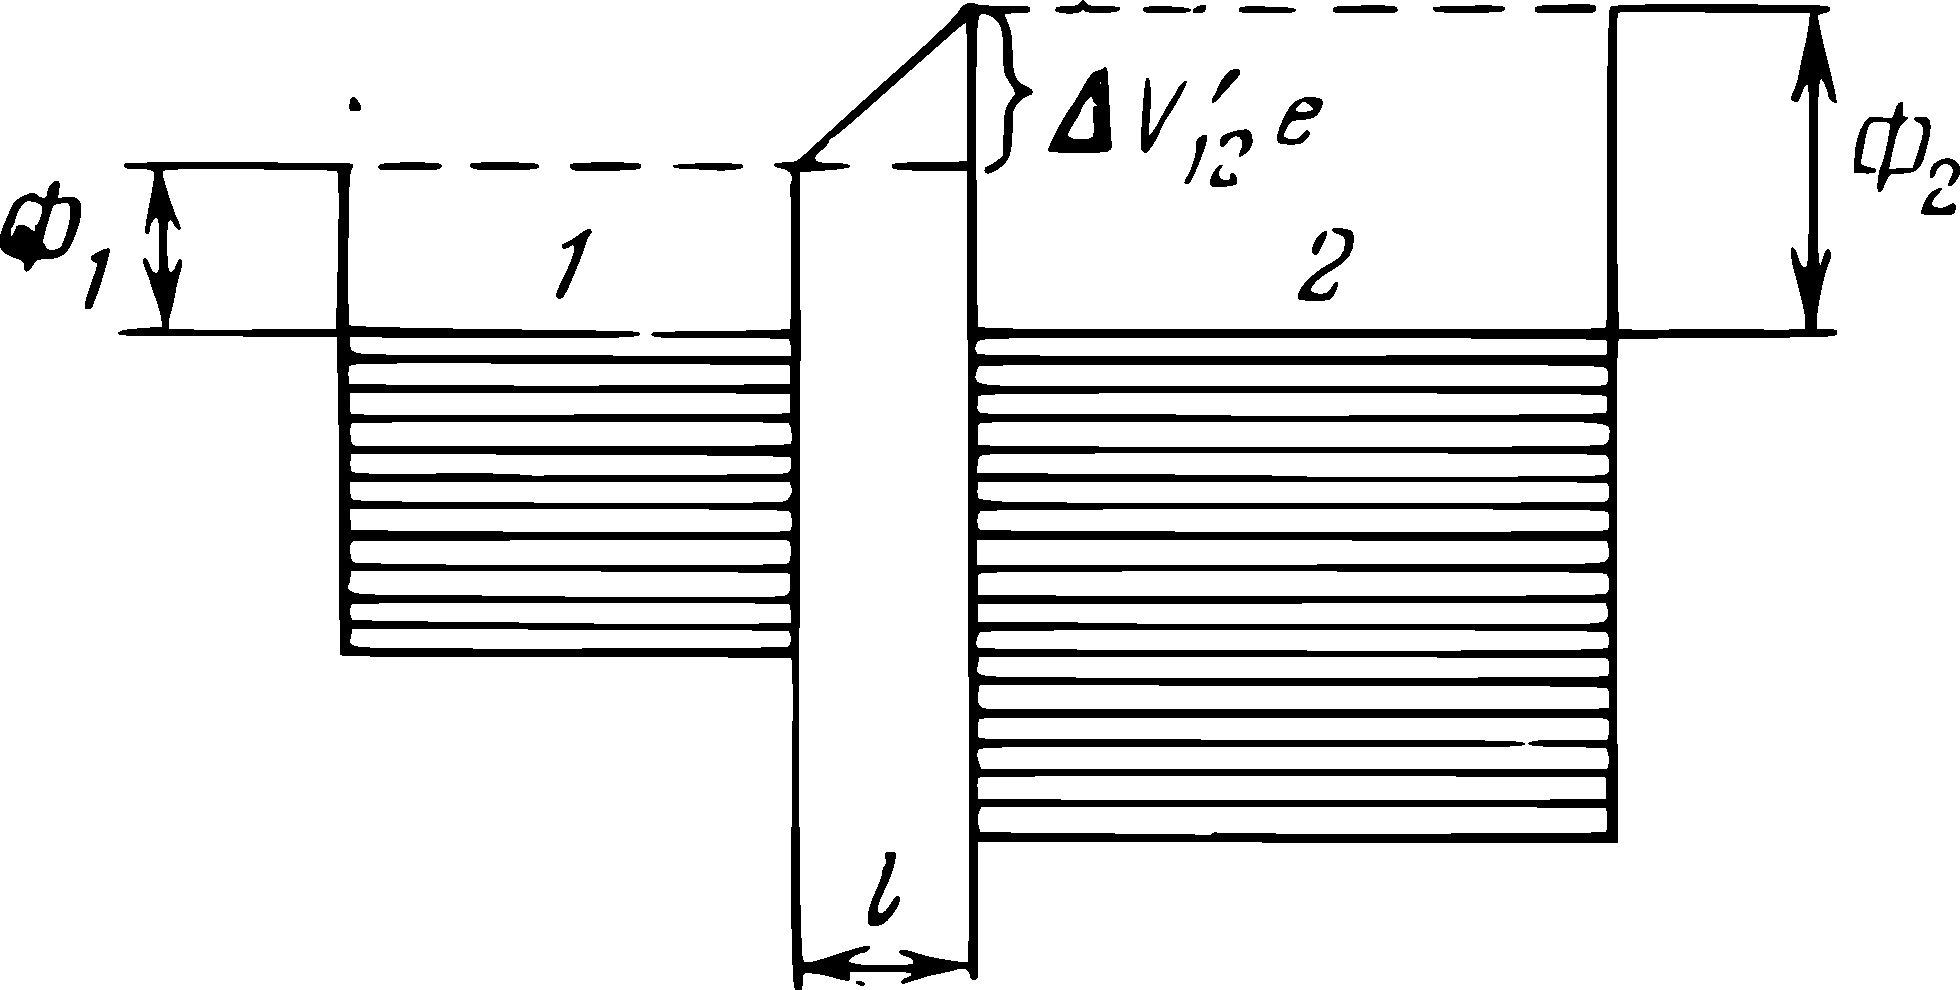
\includegraphics[width=\textwidth]{figs/ch-41/fig-41-18.pdf}
\sidecaption{Fermi levels in two metals with different work functions.\zhcap{两种逸出功不同的金属中的费米能级。}\label{fig-41-18}}
\end{marginfigure}

In the contact of the two metals shown in \figr{fig-41-17} $( \Phi_{1}< \Phi_{2})$, the electrons pass predominantly in the direction from metal $\mathit{1}$ to metal $\mathit{2}$  and they become charged positively and negatively, respectively. At the same time, a shift occurs in the energy
levels of the electrons: upward in metal $\mathit{2}$  and downward in metal $\mathit{1}$ . In a state of thermodynamic equilibrium, the Fermi levels \ssect{41.4.2} in the two metals coincide \figr{fig-41-18}.
\zhpar{在\figr{fig-41-17}所示的两金属接触情形中（$\Phi_{1} < \Phi_{2}$），电子主要沿金属 $\mathit{1}$ 指向金属 $\mathit{2}$ 的方向运动，因而两者分别带上正电和负电。同时，电子的能级发生移动：在金属 $\mathit{2}$ 中向上移，在金属 $\mathit{1}$ 中向下移。在热力学平衡状态下，两金属中的费米能级（\ssect{41.4.2}）重合（见\figr{fig-41-18}）。}



It is evident from \figr{fig-41-18} that the external contact potential difference $\Delta V_{12}'$ depends upon the work functions $\Phi_{1}$ and $\Phi_{2}$. Thus
\zhpar{由\figr{fig-41-18}可以明显看出，外接触电势差 $\Delta V_{12}'$ 取决于逸出功 $\Phi_{1}$ 和 $\Phi_{2}$。即：}
\begin{equation*}%
\Delta V_{12}' = \frac{\Phi_{1} - \Phi_{2}}{e},
\end{equation*}
The internal contact potential difference depends upon the Fermi levels in the metals. Thus
\zhpar{内接触电势差取决于两金属中的费米能级。即：}
\begin{equation*}%
\Delta V_{12} = V_{1} - V_{2} = \frac{E_{F_{1}} - E_{F_{2}}}{e},
\end{equation*}
The potential changes from $V_{1}$ to $V_{2}$ within the limits of the double electric layer \ssect{41.11.2} of thickness \figr{fig-41-19} that can be approximately assessed by the formula 
\zhpar{电势从 $V_{1}$ 变化到 $V_{2}$ 的过程发生在双电层（\ssect{41.11.2}）之内，该双电层的厚度（见\figr{fig-41-19}）可用下列公式近似估算：}
\begin{equation*}%
l = \sqrt{\frac{2 \varepsilon_{0} \Delta V_{12}'}{en_{0}}} \text{ (in SI units).}
\end{equation*}
Here $n_{0}$ is the concentration of charges in the double layer, $\varepsilon_{0}$ is the electric constant in SI units \ssect{14.2.7}, and $e$ is the electron charge.
\zhpar{式中 $n_{0}$ 为双电层中的电荷浓度，$\varepsilon_{0}$ 为 SI 单位制中的真空电容率（\ssect{14.2.7}），$e$ 为电子电荷。}

\begin{marginfigure}[-2cm] 
\centering
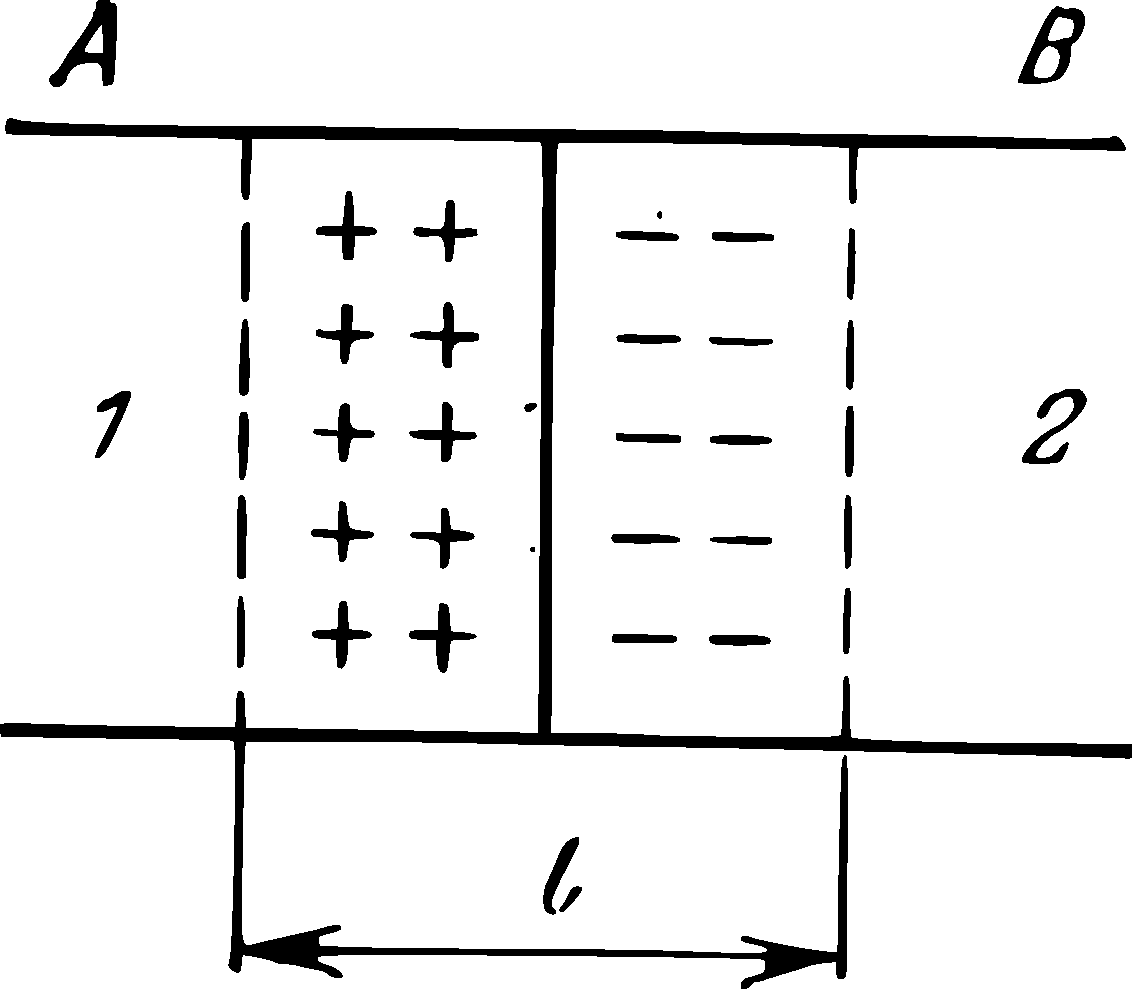
\includegraphics[width=0.8\textwidth]{figs/ch-41/fig-41-19.pdf}
\sidecaption{The double electric layer at interface of two metals.\zhcap{两金属界面处的双电层。}\label{fig-41-19}}
\end{marginfigure}

The thickness of the double layer in contacting metals is of
the order of the lattice constants in metals, and the resistivity of this layer is the same as that of the rest of the metal. Electric current passes equally well in both directions through the contact layer of two metals, and there is no \redem{rectifying (barrier-layer) effect of the contact, or function}, i.e. \redem{unilateral conduction}.
\zhpar{接触金属的双电层厚度与金属中的晶格常量为同一数量级，且该层的电阻率与金属其余部分的电阻率相同。电流可以同样容易地沿两个方向通过两金属的接触层，因此，该接触不具有整流（阻挡层）效应，即不具有\redem{单向导电性}。}



\subsection{}\label{41.11.5} Contact between a metal and an $n$-type semiconductor \ssect{41.10.6} leads to unilateral conduction of the junction. Assume that $\Phi_{1} > \Phi_{n}$ , where $\Phi_{1}$ and $\Phi_{n}$ are the work functions of the metal and the $n$-type semiconductor, respectively. The arrangement of the conduction band of the metal \ssect{41.9.2}, the completely filled band of the semiconductor and its donor levels before contact has been made are shown in \figr{fig-41-20}. After the metal makes contact with the semiconductor, electrons from the donor levels of the $n$-type semiconductor \ssect{41.10.6} move into the metal.
\zhpar{金属与 $n$ 型半导体（\ssect{41.10.6}）的接触会导致结的单向导电性。假设 $\Phi_{1} > \Phi_{n}$，其中 $\Phi_{1}$ 与 $\Phi_{n}$ 分别为金属和 $n$ 型半导体的逸出功。接触前，金属的导带（\ssect{41.9.2}）、半导体中被完全填满的能带及其施主能级的排列情况如\figr{fig-41-20}所示。金属与半导体接触后，$n$ 型半导体施主能级上的电子移入金属中。}

\begin{marginfigure}%[-3cm] 
\centering
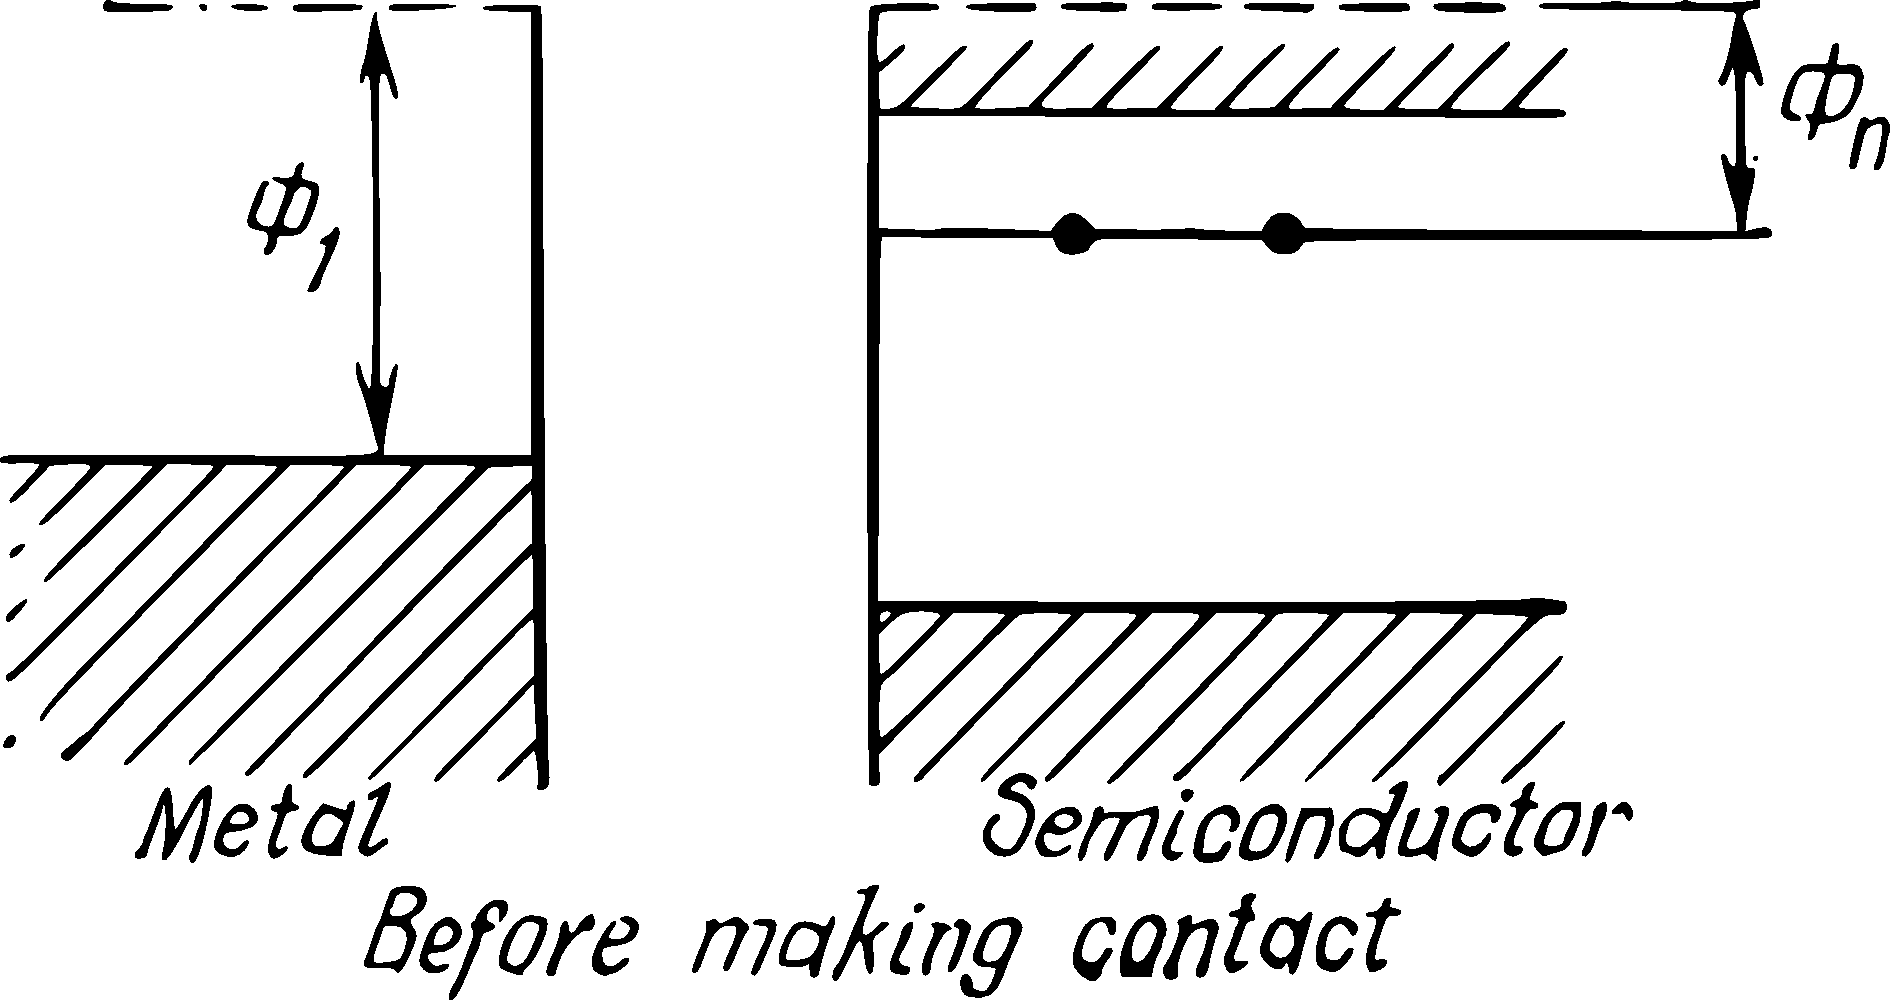
\includegraphics[width=\textwidth]{figs/ch-41/fig-41-20.pdf}
\sidecaption{Fermi levels in a metal and a semiconductor before making contact.\zhcap{接触前金属与半导体中的费米能级。}\label{fig-41-20}}
\end{marginfigure}

The charge in the contact layer \ssect{41.11.2} is positive on the side of the $n$-type semiconductor and negative on the metal side. Owing to the low electron concentration in the semiconductor in comparison to that of the metal (\SI{d15}{\per\centi\meter\cubed} instead of \SI{d22}{\per\centi\meter\cubed}), the thickness of the contact layer at the metal-semiconductor boundary is found to be approximately \num{d4} times greater than that in the metal.
\zhpar{接触层中的电荷在 $n$ 型半导体一侧为正，在金属一侧为负（\ssect{41.11.2}）。由于半导体中的电子浓度远低于金属中的电子浓度（分别为 \SI{d15}{\per\centi\meter\cubed} 和 \SI{d22}{\per\centi\meter\cubed}），金属与半导体边界处接触层的厚度约比金属中的大 \num{d4} 倍。}

\subsection{}\label{41.11.6} The small number of current carriers in the contact layer and its large thickness indicate that the resistivity of this layer is substantially greater than that of the rest of the semiconductor. Here the contact layer is called the \redem{depletion}, or \redem{space-charge, layer} (formerly called the \redem{barrier}, or \redem{blocking, layer}). The depletion layer is the basis for rectification of alternating current at a metal-semiconductor junction. When the metal is connected to the positive terminal of a source of electrical energy, and the semiconductor to the negative terminal, the external electric field is directed from the metal toward the semiconductor. 
\zhpar{接触层中载流子数目少，且厚度较大，因此该层的电阻率远大于半导体其余部分的电阻率。这一接触层称为\redem{耗尽层}，或\redem{空间电荷层}（原称\redem{阻挡层}，或\redem{阻断层}）。耗尽层是金属-半导体结对交流电进行整流的基础。当金属接电源正极、半导体接电源负极时，外电场的方向由金属指向半导体。}


In this case the electrons are pulled from the bulk of the semiconductor into the double layer. The thickness
of this layer is reduced and the conduction increases. In this
\redem{conducting direction}, electric current passes through the metal-semiconductor junction. When the external electric field is directed from the semiconductor toward the metal, the electrons are forced out of the double layer deep into the semiconductor. This increases the width and resistance of the depletion layer and in this \redem{reverse (nonconducting) direction}, the metal-semiconductor junction blocks the electric current. This unilateral conduction of the junction means that an alternating current passing through it is rectified.
\zhpar{此时，电子从半导体体内被拉入双电层中，阻挡层厚度减小，导电能力增强。沿这一\redem{导电方向}，电流可以通过金属-半导体结。当外电场方向由半导体指向金属时，电子被挤出双电层，深入半导体内部。这使耗尽层的宽度和电阻增大，在这一\redem{反向（不导电）方向}上，金属-半导体结阻断电流。结的这种单向导电性意味着，通过它的交流电会被整流。}

\begin{marginfigure}[-1cm] 
\centering
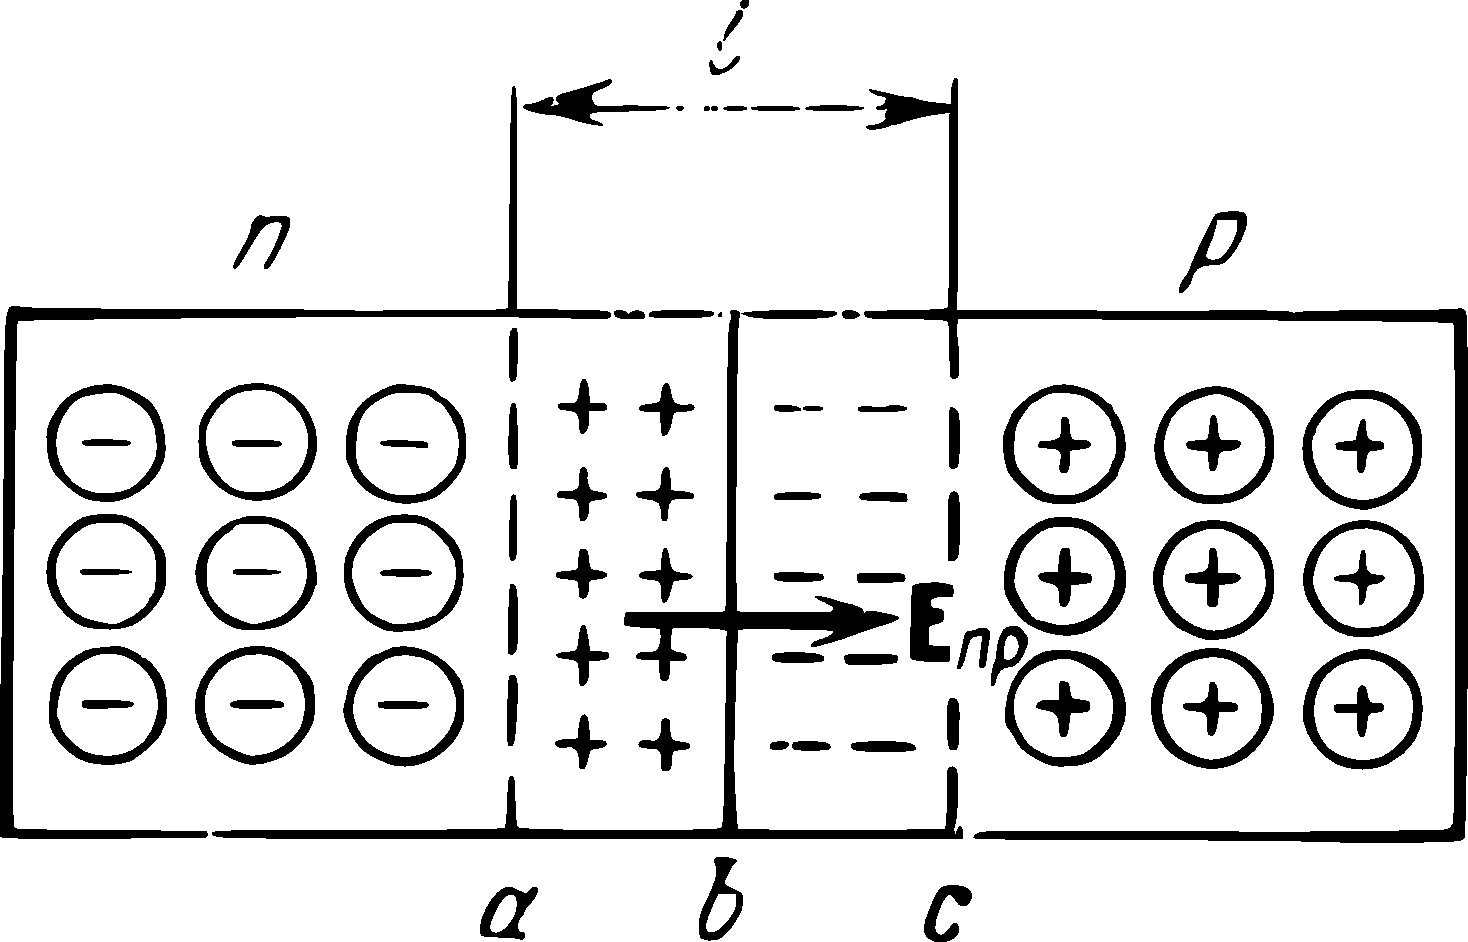
\includegraphics[width=\textwidth]{figs/ch-41/fig-41-21.pdf}
\sidecaption{The $p$-$n$ junction between $n$-type and $p$-type semiconductors.\zhcap{$n$ 型与 $p$ 型半导体之间的 $p$-$n$ 结。}\label{fig-41-21}}
\end{marginfigure}


\subsection{}\label{41.11.7} The region of contact of two semiconductors having different, $n$- and $p$-type, conduction is called an \redem{electron-hole junction} ( $p$-$n$ junction). A double electric layer \ssect{41.11.2} is
formed at a $p$-$n$ junction as a result of electron and hole motion through the interface. Electrons from the $n$-type semiconductor pass into the $p$-type semiconductor, and the holes pass in the opposite direction. This forms surplus charges of opposite sign in the $ab$ regions of the $n$-type semiconductor and $bc$ regions of the $p$-type semiconductor (\figr{fig-41-21}). 
\zhpar{具有不同导电类型（$n$ 型与 $p$ 型）的两种半导体的接触区域称为\redem{电子-空穴结}（$p$-$n$ 结）。由于电子和空穴穿过界面运动，在 $p$-$n$ 结处形成双电层（\ssect{41.11.2}）。$n$ 型半导体中的电子进入 $p$ 型半导体，同时空穴沿相反方向运动。这样，在 $n$ 型半导体的 $ab$ 区和 $p$ 型半导体的 $bc$ 区中分别形成了符号相反的过剩电荷（见\figr{fig-41-21}）。}


The double layer of thickness $l$ sets up a contact electric field with the strength $\vb{E}_{np}$ and a certain potential difference at the boundaries of the layer. This field impedes further counter migration of electrons and holes. At a definite thickness of the \emph{p-n} junction a state of equilibrium is set up, corresponding to the equalizing of the
Fermi levels in the two semiconductors. This forms an \redem{equilibrium contact layer}, which is a barrier layer \ssect{41.11.6}, having higher resistance than that of the remaining regions of the semiconductors.
\zhpar{厚度为 $l$ 的双电层在其两侧边界处建立起接触电场，其强度为 $\vb{E}_{np}$，并具有一定的电势差。该电场阻碍电子与空穴的进一步反向迁移。当 \emph{p-n} 结达到一定厚度时，便建立起平衡状态，此时两种半导体中的费米能级相等。这样就形成了\redem{平衡接触层}，它是一个阻挡层（\ssect{41.11.6}），其电阻高于半导体其余区域的电阻。}

\begin{marginfigure}[-1cm] 
\centering
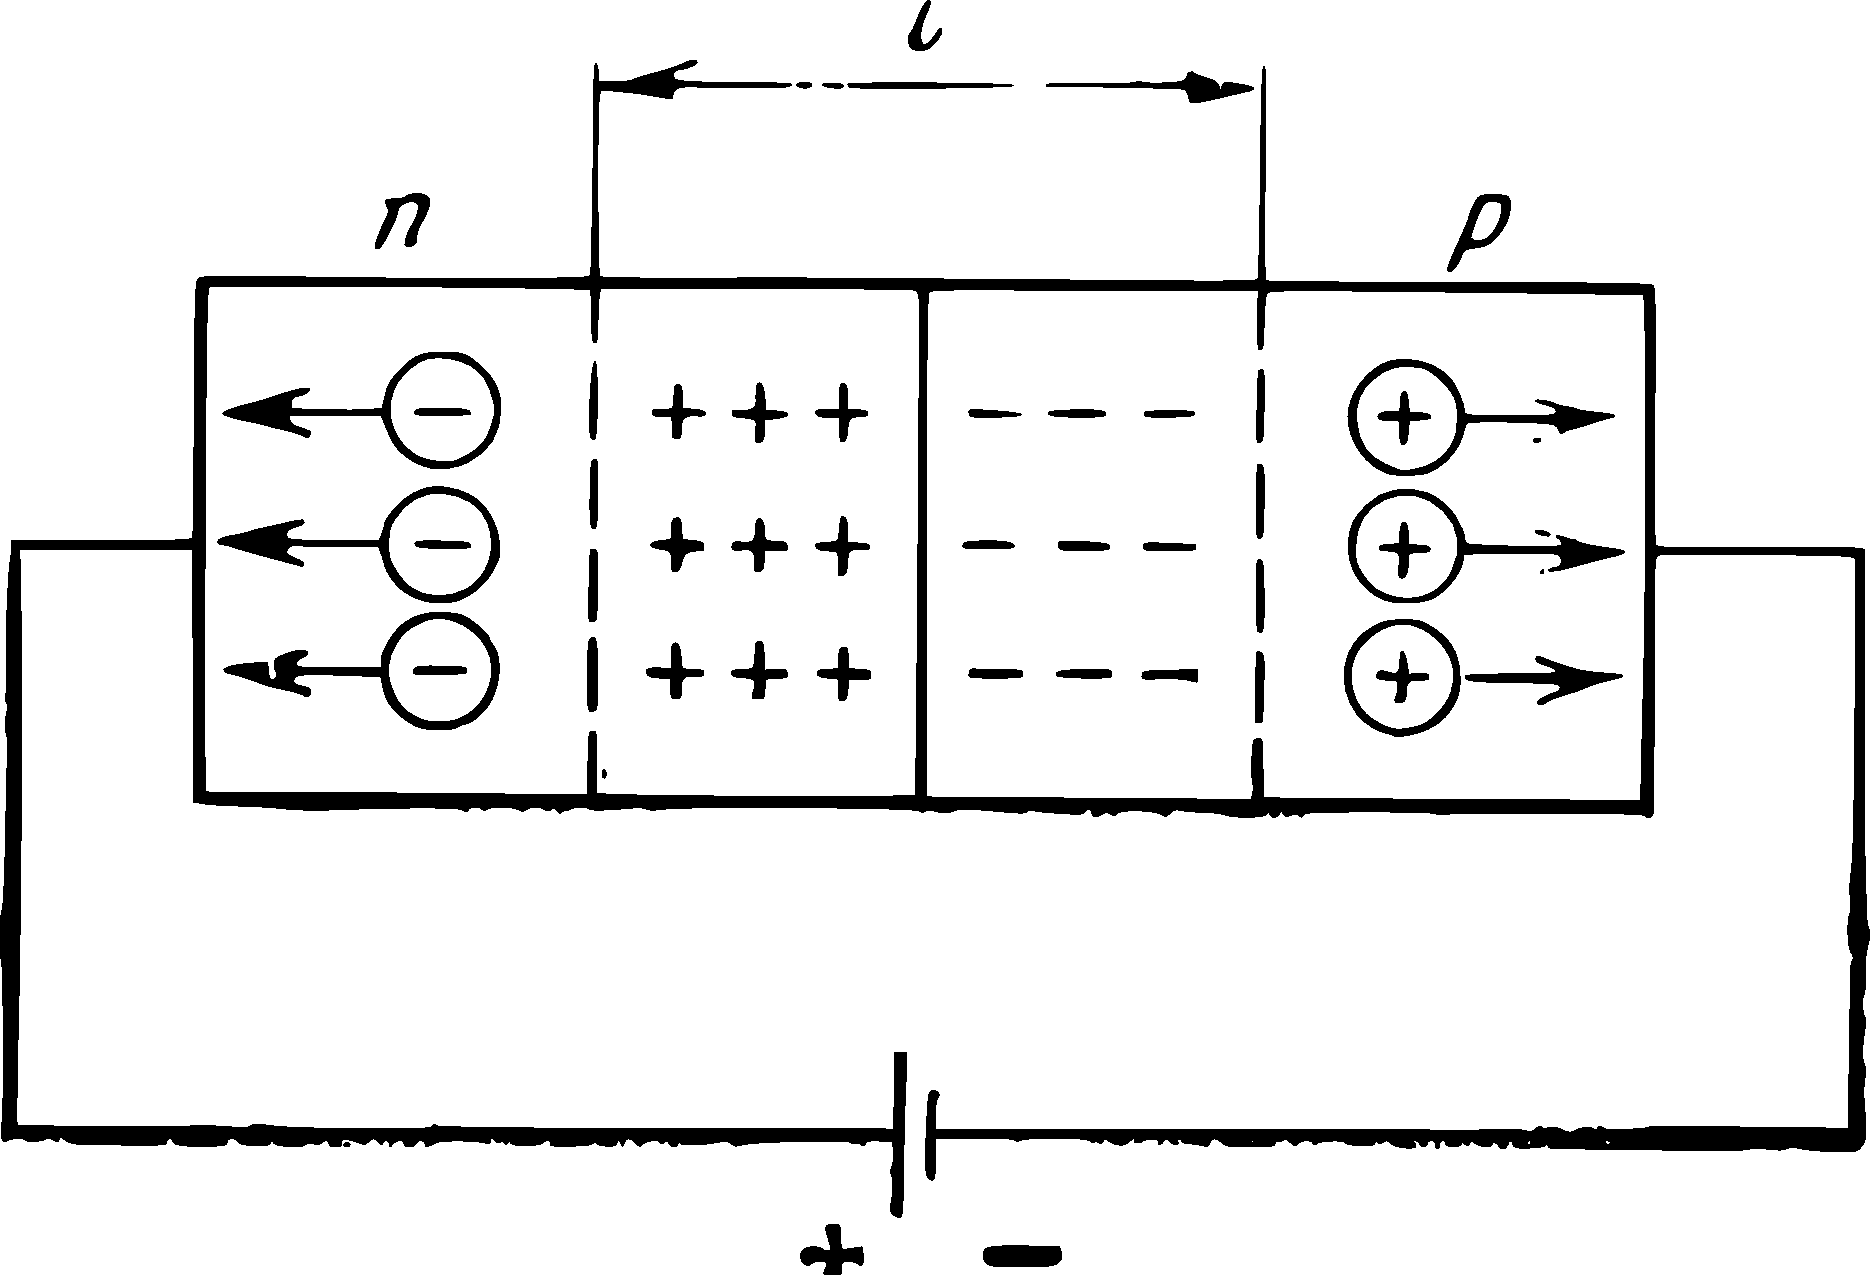
\includegraphics[width=\textwidth]{figs/ch-41/fig-41-22.pdf}
\sidecaption{The $p$-$n$ junction when connected to external applied electric field.\zhcap{接入外加电场时的 $p$-$n$ 结。}\label{fig-41-22}}
\end{marginfigure}

\subsection{}\label{41.11.8} When a \emph{p-n} semiconductor junction is connected into the external circuit of a source of electrical energy in the way shown in \figr{fig-41-22}, the external (applied) electric field, strengthening the field of the contact layer, causes electrons to migrate to the $p$-type semiconductor and holes to the $p$-type semiconductor at opposite sides of the junction. The thickness of the barrier
layer and its resistance increase. This direction of the applied electric field is said to be the \redem{reverse} one. In this direction practically no current passes through the \emph{p-n} junction. 
\zhpar{当 \emph{p-n} 半导体结按\figr{fig-41-22}所示接入电源的外电路时，外加（外部）电场加强了接触层中的电场，使电子迁移到结的 $n$ 型半导体一侧，空穴迁移到结的 $p$ 型半导体一侧（二者位于结的两侧）。阻挡层的厚度和电阻随之增大。这种外加电场的方向称为\redem{反向}。在这一方向上，电流几乎不能通过 \emph{p-n} 结。}

\begin{marginfigure}[-1cm] 
\centering
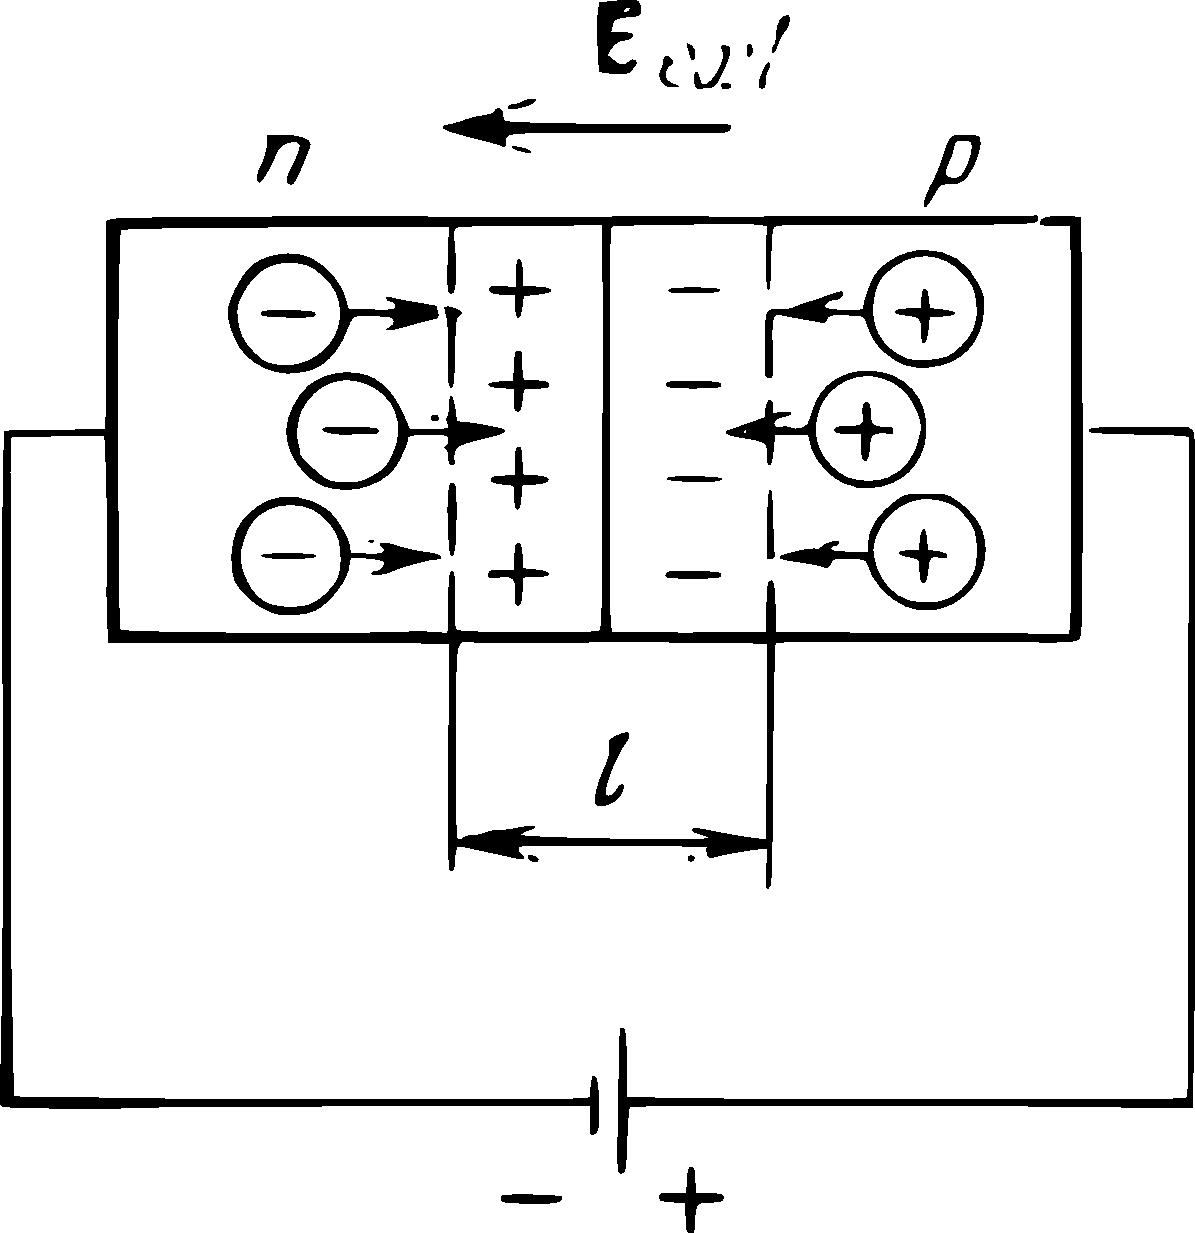
\includegraphics[width=0.8\textwidth]{figs/ch-41/fig-41-23.pdf}
\sidecaption{The $p$-$n$ junction when connected to external applied electric field is reversed.\zhcap{外加电场方向反转时的 $p$-$n$ 结。}\label{fig-41-23}}
\end{marginfigure}

When the polarity of the external applied voltage is reversed (\figr{fig-41-23}), the external electric field with the strength Eext opposes the field of the contact layer \ssect{41.11.7}. The counter motion of electrons and holes, forced by the external field to move from the bulk of the semiconductors to the region of the \emph{p-n} junction, increases the number of mobile current carriers at the junction. This reduces the thickness and resistance of the contact layer, and, in this forw.ard direction, current passes through the \emph{p-n} junction. The blocking effect of a \emph{p-n} junction is similar to the rectification of a two-electrode valve, or tube, called a diode. Accordingly, a semiconductor device containing one \emph{p-n} junction is called a \redem{semiconductor diode}. \redem{Crystal triodes}, or \redem{transistors}, contain two \emph{p-n} junctions.
\zhpar{当外加电压的极性反转（见\figr{fig-41-23}）时，强度为 $\vb{E}_{ext}$ 的外电场与接触层的电场方向相反。电子和空穴在外电场作用下，从半导体体内向 \emph{p-n} 结区域运动，从而增加了结处可移动的载流子数目。这使接触层的厚度和电阻减小，于是沿这一\redem{正向}，电流可以通过 \emph{p-n} 结。\emph{p-n} 结的阻断作用类似于二极管（一种双电极电子管）的整流作用。因此，包含一个 \emph{p-n} 结的半导体器件称为\redem{半导体二极管}。\redem{晶体三极管}，即\redem{晶体管}，包含两个 \emph{p-n} 结。}

% Local Variables:
% TeX-master: "handbook-physics"
% coding: utf-8
% End:
